%%%%%%%%%%%%%%%%%%%%%%%%%%%%%%%%%%%%%%%%%%%%%%%%%%%%%%%%%%%%%%%%%%%%%%%%%%%%%% 
%
% SIIT Thesis Template
%
% Instructions
% 1. In this file (thesis.tex) you should edit:
%    a. Thesis Data, e.g. title, author
%    b. Committee members on the Signatures page
%    c. Chapters, adding/deleting chapters
%    d. Appendices, adding/deleting appendices
%
% 2. Optionally, in this file you may edit:
%    a. Packages, adding/deleting required LaTeX packages
%    b. Authors Commands, adding/deleting your own LaTeX commands
%    c. Remove the inclusion of acrynoms
%    d. References, to switch from using BibTeX to a .bbl file
% 
% 3. The main content of the thesis should be in the following files:
%    a. ack.tex
%    b. abstract.tex
%    c. acronyms.tex (optional)
%    d. chapter1.tex, chapter2.tex, ...
%    e. appendixA.tex, appendixB.tex, ...
%    f. refs.bib (if using BibTeX) or refs.tex (if manual editing refs)
%
% \SVN $Revision: 840 $
% \SVN $Author: sgordon $
% \SVN $Date: 2014-05-12 13:39:14 +0700 (Mon, 12 May 2014) $
% \SVN $URL: https://sandilands.info/svn/Common/Styles/siitthesis/thesis.tex $
%
%%%%%%%%%%%%%%%%%%%%%%%%%%%%%%%%%%%%%%%%%%%%%%%%%%%%%%%%%%%%%%%%%%%%%%%%%%%%%% 
\documentclass[12pt,a4paper,oneside]{book}

%%%%%%%%%%%%%%%%%%%%%%%%%%%%%%%%%%%%%%%%%%%%%%%%%%%%%%%%%%%%%%%%%%%%%%%%%%%%%% 
%
% Packages
% (add/remove packages as needed)
%
%%%%%%%%%%%%%%%%%%%%%%%%%%%%%%%%%%%%%%%%%%%%%%%%%%%%%%%%%%%%%%%%%%%%%%%%%%%%%% 

% Required packages for thesis layout (do not remove)
\usepackage{siitthesis} % Commands for formatting according SIIT thesis style

% Other packages (add/delete packages as desired)
\usepackage{graphicx}
\usepackage{svn}
\usepackage[plainpages=false]{hyperref}
\usepackage{url}
\usepackage{amsmath}
\usepackage{amssymb}
\usepackage{amsthm}
\usepackage{tikz}



%%%%%%%%%%%%%%%%%%%%%%%%%%%%%%%%%%%%%%%%%%%%%%%%%%%%%%%%%%%%%%%%%%%%%%%%%%%%%% 
%
% Thesis Data
% (edit each field)
%
%%%%%%%%%%%%%%%%%%%%%%%%%%%%%%%%%%%%%%%%%%%%%%%%%%%%%%%%%%%%%%%%%%%%%%%%%%%%%% 
% Thesis Title in mixed case
\newcommand{\thesistitle}{High performance  Opportunistic Routing Algorithms for power constrained nodes with message delivery deadline in Sparse network environment}

% Student name (author of the thesis)
\newcommand{\thesisauthor}{Jiradett Kerdsri}

% Degree that this thesis is for
\newcommand{\thesisdegree}{Doctor of Philosophy Program in Engineering and Technology}

% Month and year of thesis publication (obtained from SIIT)
\newcommand{\thesisdate}{December 2014}

% Academic year for thesis submission
\newcommand{\thesisyear}{2014}

% Institute/department
\newcommand{\thesisinstitute}{Sirindhorn International Institute of Technology}

% University
\newcommand{\thesisuni}{Thammasat University}

% Degrees that student already has; separate degrees with \\
\newcommand{\thesispastdegrees}{Bachelor of Civil Engineering, Royal Thai Air Force Academy, 1999\\Master of Science in Computer, Naval Postgraduate School, 2003\\Master of Geographic Information Technology, University of Melbourne, 2009}


%%%%%%%%%%%%%%%%%%%%%%%%%%%%%%%%%%%%%%%%%%%%%%%%%%%%%%%%%%%%%%%%%%%%%%%%%%%%%% 
%
% Authors Commands
% (optionally include your own LaTeX commands here; some examples are
%  included)
%
%%%%%%%%%%%%%%%%%%%%%%%%%%%%%%%%%%%%%%%%%%%%%%%%%%%%%%%%%%%%%%%%%%%%%%%%%%%%%% 

%% Format of code listing fors ML (package: listings)
\lstdefinelanguage[]{CPNML}[]{ML}{morekeywords={colset}}
\lstset{%
language=CPNML,
basicstyle=\footnotesize,
columns=flexible,
}

%% Note for editor/advisor, e.g. \ednote{Add a new paragraph}
\newcommand{\ednote}[1]{\textbf{Edit: #1}}

%% Graphics path and formats (package: graphicx). Add directories that contain
%% figures that you want to include
\graphicspath{{./}{./figures/}}


%%%%%%%%%%%%%%%%%%%%%%%%%%%%%%%%%%%%%%%%%%%%%%%%%%%%%%%%%%%%%%%%%%%%%%%%%%%%%% 
%
% Title Page
% (do not edit)
%
%%%%%%%%%%%%%%%%%%%%%%%%%%%%%%%%%%%%%%%%%%%%%%%%%%%%%%%%%%%%%%%%%%%%%%%%%%%%%% 
\begin{document}
\frontmatter
\setlength{\parskip}{0pt plus1pt minus1pt}

\pagestyle{empty}
\begin{center}
\vspace*{6mm}
\begin{spacing}{1.4}
\textbf{\Large\MakeUppercase\thesistitle}
\end{spacing}
\vspace*{35mm}
\textbf{BY}\\
\vspace*{17mm}
\textbf{\MakeUppercase\thesisauthor}
\vfill
\begin{spacing}{1.3}
\textbf{
A THESIS SUBMITTED IN PARTIAL FULFILLMENT OF\\
THE REQUIREMENTS FOR THE DEGREE OF\\
\MakeUppercase\thesisdegree\\
\MakeUppercase\thesisinstitute\\
\MakeUppercase\thesisuni\\
ACADEMIC YEAR \thesisyear\\
}
\end{spacing}
\end{center}
\newpage


%%%%%%%%%%%%%%%%%%%%%%%%%%%%%%%%%%%%%%%%%%%%%%%%%%%%%%%%%%%%%%%%%%%%%%%%%%%%%% 
%
% Signatures
% (only edit the table of thesis committee)
%
%%%%%%%%%%%%%%%%%%%%%%%%%%%%%%%%%%%%%%%%%%%%%%%%%%%%%%%%%%%%%%%%%%%%%%%%%%%%%% 
\pagestyle{plain}
\setcounter{page}{1}
\addcontentsline{toc}{section}{Signature Page}
\vspace*{2mm}
\begin{center}
\textbf{\MakeUppercase\thesistitle}\\
\vspace*{17mm}
A Thesis Presented\\
\vspace*{8mm}
By\\
\vspace*{2mm}
\MakeUppercase\thesisauthor\\
\vspace*{12mm}
\begin{spacing}{1.3}
Submitted to\\
\thesisinstitute\\
\thesisuni\\
In partial fulfillment of the requirement for the degree of\\
\MakeUppercase\thesisdegree
\end{spacing}
\end{center}
\vfill
~Approved as to style and content by\\[-2ex]
\begin{table}[h]
\setlength{\tabcolsep}{0.7ex}
\begin{tabular}{lll}
%%============================================================================
%% Example for Masters Thesis
%Advisor and&& \\ \cline{3-3}
%Chairperson of Thesis Committee    &&Assoc. Prof. Steven Gordon, Ph.D.\\[3ex]
%Committee Member and&&\\ \cline{3-3}
%Chairperson of Examination Committee&&Assoc.\ Prof.\  Komwut Wipusitwarakun, Ph.D.\\[3ex]
%Committee Member&&\\ \cline{3-3}
%&&Asst.\ Prof.\ Somsak Vanit-Anunchai, Ph.D.\\[3ex]
%%============================================================================
%% Example for PhD Thesis
Advisor and&& \\ \cline{3-3}
Chairperson of Thesis Committee&&Assoc.\ Prof.\  Komwut Wipusitwarakun, Ph.D.\\[3ex]
Committee Member and&&\\ \cline{3-3}
Chairperson of Examination Committee&&Assoc. Prof. Steven Gordon, Ph.D.\\[3ex]
Committee Member&&\\ \cline{3-3}
&&Asst.\ Prof.\ Prapun Suksompong, Ph.D.\\[3ex]
Committee Member&&\\ \cline{3-3}
&&Asst.\ Prof.\ Somsak Kittipiyakul, Ph.D.\\[3ex]
External Examiner:&&Prof. xx xxxx, Ph.D.\\[3ex]
%%============================================================================
\end{tabular}
\end{table}\\
\centerline{\MakeUppercase\thesisdate}
\newpage


%%%%%%%%%%%%%%%%%%%%%%%%%%%%%%%%%%%%%%%%%%%%%%%%%%%%%%%%%%%%%%%%%%%%%%%%%%%%%% 
%
% Acknowledgement
% (do not edit here; instead edit the file ack.tex)
%
%%%%%%%%%%%%%%%%%%%%%%%%%%%%%%%%%%%%%%%%%%%%%%%%%%%%%%%%%%%%%%%%%%%%%%%%%%%%%% 
\addcontentsline{toc}{section}{Acknowledgments}
\chapter*{Acknowledgments}
% Acknowledgments. 
%
% \SVN $Revision: 840 $
% \SVN $Author: sgordon $
% \SVN $Date: 2014-05-12 13:39:14 +0700 (Mon, 12 May 2014) $
% \SVN $URL: https://sandilands.info/svn/Common/Styles/siitthesis/ack.tex $

This thesis is the end of my long journey obtaining a doctorate degree in Engineering and Technology. 
I can honestly state that it would not have been possible without the support from several people.

First of all, I would like to express my sincere gratitude to my advisor Assoc. Prof. Komwut Wipusitwarakun for his continuous support of my Ph.D. study and research, for his patience, motivation, enthusiasm, and immense knowledge.
At every step of my thesis, he guided me with his profound knowledge, insight and wisdom.
I would like to express my deep gratitude to him for being such a great advisor. 

Besides my advisor, I would like to thank the rest of my thesis committee: Assoc. Prof. Steven Gordon, Asst. Prof. Prapun Sukompong and Asst. Prof. Somsak Kittipiyakul, for their encouragement, insightful comments, and hard questions. I also would like to express my appreciation to my external examiner, Prof. SEAH, Khoon Guan Winston, for his useful suggestions and helpful comments. 
I am thankful for all faculty members in the school of Information and Computer Technology, SIIT, for their support, valuable comments and suggestions on the research.

I also would like to thank to my colleague in Information Technology of SIIT and Defence Technology Institute (DTI), for stimulating discussions and all the fun we had studying together. 
I appreciate their efforts in helping me solving several problems I faced through this thesis work.
Thanks for their concern, mind power and encouragement all the time.
Especially my supervisor at DTI, Asst. Prof. Tawiwat Veeraklaew, who inspires me and also recommended me to pursue my Ph.D. at SIIT.

Finally, my deep gratitude goes to my family, my mother and sister.
I am very grateful to them for standing by me in everything I have done and giving me whatever they can.
They have always provided me continuous support, encouragement and their love.
I believe that nothing would be possible without the presence of them and the peaceful family environment they provided me during my life.
Even though my father already passed away but he had always been my greatest teacher who inspire me about higher education. 
I would like to dedicate this thesis to them.
\newpage


%%%%%%%%%%%%%%%%%%%%%%%%%%%%%%%%%%%%%%%%%%%%%%%%%%%%%%%%%%%%%%%%%%%%%%%%%%%%%% 
%
% Abstract
% (do not edit here; instead edit the file abstract.tex)
%
%%%%%%%%%%%%%%%%%%%%%%%%%%%%%%%%%%%%%%%%%%%%%%%%%%%%%%%%%%%%%%%%%%%%%%%%%%%%%% 
\addcontentsline{toc}{section}{Abstract}
\chapter*{Abstract}
\begin{center}
\MakeUppercase\thesistitle\\
\vspace*{7mm}
by\\
\vspace*{7mm}
\thesisauthor
\end{center}
\vspace*{0mm}
\begin{flushleft}
\thesispastdegrees
\vspace*{5mm}
\end{flushleft}

% Abstract. 
%
% \SVN $Revision: 840 $
% \SVN $Author: sgordon $
% \SVN $Date: 2014-05-12 13:39:14 +0700 (Mon, 12 May 2014) $
% \SVN $URL: https://sandilands.info/svn/Common/Styles/siitthesis/abstract.tex $

Opportunistic Network (OppNet) is a challenge network exploiting contact opportunities and node mobility to route the messages even a complete path from source to destination never exists.
%%
The example applications for such extreme networks are in the environments of battlefield network, wildlife monitoring or disaster response  where movements are random with highly intermittent connections. 
%5
This opportunistic routing relies on store-carry-forward paradigm, which a data holing node such as source or neighbor node can carry the data and find an opportunity to forward data by discovering its nearest neighbor node and uses it to forward messages toward the destination node.
%5
However, the performance of opportunistic routing algorithm largely depends on several factors such as limited knowledge of contact behavior or the density of mobile nodes.
%%
The problems arise in sparse network environment with limited delivery deadline, which results in low delivery ratio.
%5
Several researches attempted to address the sparseness problems by a special node such as data mules or message ferries.
%5
Nevertheless, proposed solutions impractical under some application environments especially with limited power constraints.
%5

In order to improve the delivery ratio in such sparse network circumstances while maintaining the energy consumption, we proposed a novel Dynamic Rendezvous based Routing Algorithm on Sparse Opportunistic Network Environment where the rendezvous concept is implemented to address the problem of routing in such extreme environment.
%5
In addition, we proposed DORSI: Data-wise Opportunistic Routing with Spatial Information where the significant of data content is accounted for the forwarding algorithm and decision of the nodes. 
%5
This DORSI can improve the delivery ratio for the important messages, thus increase the delivery ratio if the weight of each class is accounted.
%5
In those algorithms, our common objective is to increase the network performance such as delivery ratio or composite matrices under given circumstances.
%%
We also present intensive simulation results regarding the performance comparison of the proposed algorithms with the tradition OppNet routing algorithms.



\newpage


%%%%%%%%%%%%%%%%%%%%%%%%%%%%%%%%%%%%%%%%%%%%%%%%%%%%%%%%%%%%%%%%%%%%%%%%%%%%%% 
%
% Table of Contents, Figures and Tables
% (comment/uncomment any tables/lists that you desire)
%
%%%%%%%%%%%%%%%%%%%%%%%%%%%%%%%%%%%%%%%%%%%%%%%%%%%%%%%%%%%%%%%%%%%%%%%%%%%%%% 
\addcontentsline{toc}{section}{Table of Contents}
\tableofcontents
\newpage
\addcontentsline{toc}{section}{List of Figures}
\listoffigures
\newpage
\addcontentsline{toc}{section}{List of Tables}
\listoftables
\newpage
\addcontentsline{toc}{section}{List of Listings}
\lstlistoflistings
\newpage


%%%%%%%%%%%%%%%%%%%%%%%%%%%%%%%%%%%%%%%%%%%%%%%%%%%%%%%%%%%%%%%%%%%%%%%%%%%%%% 
%
% List of Acronyms
% (do not edit here; instead edit the file acronyms.tex)
%
%%%%%%%%%%%%%%%%%%%%%%%%%%%%%%%%%%%%%%%%%%%%%%%%%%%%%%%%%%%%%%%%%%%%%%%%%%%%%% 
\addcontentsline{toc}{section}{List of Acronyms}
\chapter*{List of Acronyms}
% Acronyms/abbreviations. The example is a borderless table of two left-
% aligned columns. Add/edit rows as needed. If the list is over multiple
% pages, then you may need to manually split it into multiple tabuler
% environments.
%
% \SVN $Revision: 840 $
% \SVN $Author: sgordon $
% \SVN $Date: 2014-05-12 13:39:14 +0700 (Mon, 12 May 2014) $
% \SVN $URL: https://sandilands.info/svn/Common/Styles/siitthesis/acronyms.tex $

\begin{tabular}{ll}
BWMNs & Battlefield Wireless Military Networks\\
DTNs & Delay/Disruptive Tolerant Networks\\
EMNs & Exotic Media Networks\\
GPS & Global Positioning System\\
ICNs & Intermittently Connected Networks\\
IETF & Internet Engineering Task Force\\
IRTF & Internet Research Task Force\\
IPN & Inter-Planetary Network\\
MANET & Mobile Ad-Hoc Network\\
MWSNs & Mobile Wireless Sensor Networks\\
OppNet(s) & Opportunistic Network(s)\\
OR & Opportunistic Routing\\
PSWN & Pocket-SwitchedWireless Networks\\
QoS & Quality of Service\\
RF & Radio Frequency
SANs \& Sensor/Actuator Networks\\
SCF & Store-Carry-Forward routing\\
VANETs & Vehicular Ad-Hoc Network\\
WSNs & Wireless Sensor Networks\\
\end{tabular}


\newpage


%%%%%%%%%%%%%%%%%%%%%%%%%%%%%%%%%%%%%%%%%%%%%%%%%%%%%%%%%%%%%%%%%%%%%%%%%%%%%% 
%
% Chapters
% (edit the files chapter1.tex, chapter2.tex, ...)
%
%%%%%%%%%%%%%%%%%%%%%%%%%%%%%%%%%%%%%%%%%%%%%%%%%%%%%%%%%%%%%%%%%%%%%%%%%%%%%% 
\mainmatter
\setlength{\parindent}{0.25in}
\clearpage
%!TEX root = thesis.tex
\chapter{Introduction}
\label{intro}
% \SVN $Revision: 838 $
% \SVN $Author: sgordon $
% \SVN $Date: 2014-05-12 13:30:42 +0700 (Mon, 12 May 2014) $
% \SVN $URL: https://sandilands.info/svn/Common/Styles/siitthesis/chapter1.tex $

Opportunistic networks are one of the most interesting evolutions of multi-hop wireless network especially in Mobile Ad-hoc Networks (MANETs).
%%
On the one hand, MANETs characterize an approach to conceal the mobility of the nodes by constructing \emph{stable} end-to-end paths for communications. 
%%
On the other hand, opportunistic network consider a problem of node mobility in MANETS as an opportunity to exploit \cite{Conti2014}.
%% 
In this network scheme, mobile nodes are enabled to communicate with each other even without connected route and prior network topology knowledge \cite{Pelusi2006}.
%%
Several concepts behind opportunistic network come from the studies on DTN that led to the specification of its architecture \cite{Conan2008,Yu2012,Rongxing2010,Schurgot2012}. 
%%
Source and destination nodes might never be fully connected at the same time in opportunistic network, so the forwarding algorithms in such networks follow a \emph{store-carry-forward} paradigm \cite{Yamamura2011,Jie2007,Jie2007a} by exploiting opportunistically connections arising from mobility nature of nodes and temporary wireless links. 
%%
Typical algorithms differ based on their decisions as how to forwards the data, at what time the data is forwarded and to whom the data is sent \cite{Joe2010}. 
%%
However, the decision algorithms of what the data to sent has never fully implemented. 
%%
Messages are en route between the sender and the destination on the routes that dynamically built, and any possible node can opportunistically be used as next hop, provided it is likely to bring the message closer to the final destination .
%%
With the opportunistic paradigm, a data can be delivered from a source toward a destination by exploiting the sequence of connectivity graphs generated by the mobility of the nodes \cite{Acer20111,Ferretti2013}
%%
In the real world scenario, there are several examples of such networks implementing for specific applications. 
%%
These applications are mainly based on the environments causing the extreme networks scheme.
%%
The interferences and jamming in the military operations are the example of opportunistic environments, thus there are many opportunistic routing proposals for military domain \cite{Kerdsri2012a,Scott2005,Kidston2012,Haillot2009}.




%=============================================================================
\section{Problem Statement}
\label{intro:Problem Statement}
%=============================================================================
In this store-carry-forward paradigm, the network suffers the decreasing of performance in the insufficient collaborating nodes environment \cite{Nousiainen2013,Spyropoulos2010}
Since the node holding the data requires next-hop neighbor nodes to forward the data to, the sparse network environment is normally unable to satisfy opportunistic routing.
As a result, there is a need for an innovative protocol design to address this deficiency of OppNets.

In addition, none of the traditional routings in OppNets concern about the data content of the messages. 
If the significance of data is considered as the performance matrix, the network effectiveness of OppNets also drops in sparse network. 
In several environments, it is essential that the important messages from source to the destination nodes should be specially treated in order to guarantee deliverable.
Therefore, it is crucial to implement a new protocol to increase the delivery ratio of important data for critical data network such as military tactical network or disaster relief network.

In this thesis, we study the algorithms to address the perform deficiency in sparse opportunistic network environment.
In each approach, we use different routing techniques and work on different OppNets scenarios, however our common aim is to increase the performance in sparse network.
%=============================================================================
\section{Objective and Scope}
\label{intro:Objective and Scope}
%=============================================================================
Objective of this research is to increase the network performance in OppNets especially the delivery ratio and other key composite matrices performance index in different schemes.
The scope of this research is based on the assumption of mobile nodes and environment in different network schemes that elaborate in each proposed approaches.

%=============================================================================
\section{Proposed Approaches}
\label{intro:Proposed Approaches}
%=============================================================================
From aforementioned problem statements, this thesis proposed the following approaches:
\begin{itemize}
  \item %DORSI: Data-wise Opportunistic Routing with Spatial Information
  We proposed a protocol to classify the messages based on the information sensitivity concept along with nodes prioritization technique corresponding to the their delivery probability computed by spatial data. 
  This protocol classifies the messages according to their significant level, security level and deadline relative to the sensitivity level of data. 
  In addition we adapts the geographical routing technique to select the best candidate node to forward the messages to the destination. 
  Simulation experiments clearly illustrate that two key performance indexes: (1) effective delivery ratio and (2) effective replication ratio remarkably improve over the traditional Epidemic routing. 
  
  
  \item %Dynamic Rendezvous based Routing Algorithm on Sparse Opportunistic Network Environment 
In order to address the problem in sparse network, we proposed the use of Rendezvous based concept in order to maintain the messages in one place as long as the messages are delivered. 
By injected a special node $N_{rv}$ into the network, the gap between time and space domain of mobile nodes are bridge. Messages can be transferred from source node to destination node even if they are not in the same location at the same time with the help of rendezvous node. 
The results clearly show that the delivery ratio of Rendezvous based protocol significant improve over Epidemic protocol especially in the sparse environment.
\end{itemize}

%=============================================================================
\section{Our Contributions}
\label{intro:Our Contributions}
%=============================================================================
This thesis contains five chapters.
Chapter 1 gives an introduction of the research.
In addition, the problem statement, objective and scope, and proposed approaches are included in this chapter.
In Chapter 2 the background and related works on opportunistic networks are provided.
Chapter 3 describes our message prioritization technique to differentiate the routing based on the significant level of messages.
The details of proposed method, simulation model, and performance evaluation are included in this chapter.
Chapter 4 presents our approach of using the rendezvous place concept to overcome the limitation of insufficient collaborating nodes in sparse network environment.
The details of proposed method, simulation model, and performance evaluation are included in this chapter.
Chapter 5 includes the discussion, the conclusion and the recommendations for future studies.
\chapter{Background and Related Work}
\label{bg}
% \SVN $Revision: 838 $
% \SVN $Author: sgordon $
% \SVN $Date: 2014-05-12 13:30:42 +0700 (Mon, 12 May 2014) $
% \SVN $URL: https://sandilands.info/svn/Common/Styles/siitthesis/chapter2.tex $

Recently, wireless networking are witnessing several deployments in various extreme environments where they usually suffer from different levels of link disruptions depending on the severity of the operations. 
Commonly, these networks are known as Intermittently Connected Networks (ICNs). 
An ICNs, also known as a Challenged Network, is an infrastructure-less wireless network that supports the proper functionality of the wireless applications operating in stressful environments, where excessive delays and no existence of end-to-end path(s) between any arbitrary source-destination pair, result from highly repetitive link disruptions \cite{Khabbaz2012}.
In order to handle ICNs, the Internet Engineering Task Force (IETF) \cite{Cerf2007} proposed an architecture called Delay-/Disruption-Tolerant Networks (DTNs).
DTNs can basically be categorized into 3 types: scheduled networks, predictable networks and opportunistic networks.
In this thesis, we focus on the research on the most extreme case of DTNs which is the opportunistic networks.

This chapter gives the background knowledge of this thesis. 
The background of Delay Tolerant Networks is presented in Section~\ref{bg:Delay Tolerant Networks}. 
Additionally, an explanation of Opportunistic Networks is presented in Section~\ref{bg:Opportunistic Networks}. 
%=============================================================================
\section{Delay Tolerant Networks}
\label{bg:Delay Tolerant Networks}
%=============================================================================
DTNs is an overlay architecture with an aim to operate over the protocol stacks of the ICNs and enable gateway functionality between them through the use of storage capacity, a variety of protocol techniques, replication and parallel forwarding, forward error correction and many other techniques for overcoming the impairments of communication  \cite{Khabbaz2012}.
DTNs enable the transferring of data in extremely challenging environments where networks are assumed to experience frequent, long-duration partitioning and may have no end-to-end connectivity between source and destination \cite{Liu2011}. 
Therefore, the timer and acknowledgement mechanisms of the traditional TCP/IP protocol definitely fail in such circumstances \cite{Souza2010}.
In addition, the routing algorithms designed for Mobile Ad hoc NETworks (MANETs) can not perform effectively under aforementioned constraints as well, since the availability of contemporaneous end-to-end connectivity is essential for conventional routing algorithms \cite{Yue2013}.

Basically the types of DTNs can be classified in 3 categories: scheduled networks, predictable networks and opportunistic networks as seen in Figure~\ref{fig:bg:Type of DTN}.
In DTNs, predictable and scheduled networks are the common aim in designing the routing protocols in the highly disruptive environments such as Interplanetary Internet (IPN) \cite{Burleigh2003} where the contact time is not completely random but in periodic interval.
In the thesis, we study in the most extreme case of DTNs which is the opportunistic networks where the contact time is undetermined along with stochastic movements.


\begin{figure}
\centering
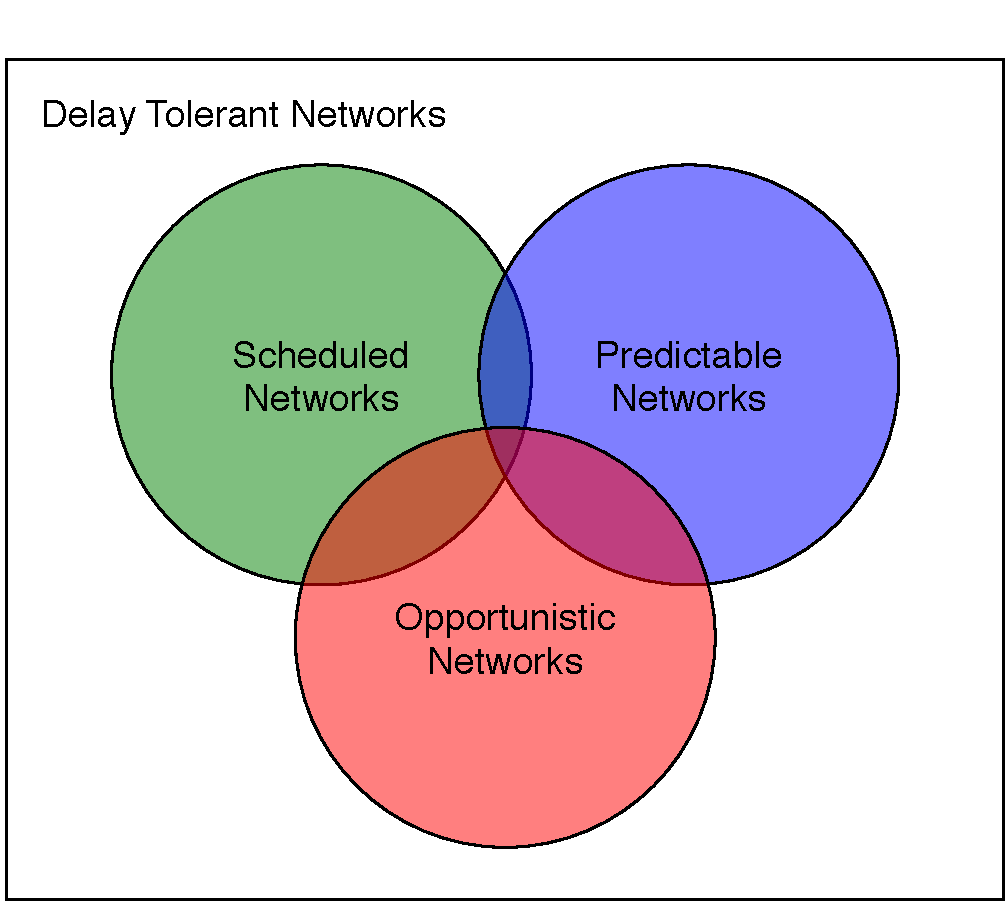
\includegraphics[width=0.5\columnwidth]{Figures/TypeOfDTN.pdf}
\caption{Types of DTN}
\label{fig:bg:Type of DTN}
\end{figure} 


%=============================================================================
\section{Opportunistic Networks}
\label{bg:Opportunistic Networks}
%=============================================================================
In fact, Opportunistic networks focus on mobile ad-hoc DTNs, where tolerant delayed routes between the source and destination are built dynamically.
However, OppNets is different from MANETs that it does not assume the existing end-to-end connectivity.
Therefore, instead of depending on end-to-end MANETs routing protocols, the messages are delivered through one hop data transmission among opportunistic node encounters with intermediate node storage and mobility, called \textit{Store-Carry-Forward paradigm} \cite{Hu2009}. 
In essential, there are three common steps of routing in OppNet \cite{Hsu2011}:
\begin{itemize}
	\item Broadcast the messages to candicate relayed nodes.
	\item Select the best candidate node.
	\item Forward the messages.
\end{itemize}



%=============================================================================
\subsection{Opportunistic Routing}
\label{bg:Opportunistic Networks:Opportunistic Routing}
%=============================================================================
In this opportunistic routing, the nodes can exchange data in a spontaneous manner whenever they come in close.
If there is no direct connection from source to destination, data holding nodes will discover their nearest neighbor nodes to forward messages toward the destination node.
Thus, this opportunistic route is determined at each hop when messages traverse through different hops.
In this routing scheme, mobile nodes are normally equipped with local knowledge of the best nodes around them to determine the best path to transmit the messages with this knowledge.
In the case of such nodes absence, the node currently holding the message simply stores the messages and wait for an opportunity to forward the packets.
This  infrastructure-less wireless network environment requires common 2 factors to facilitate the opportunistic routing \cite{Poonguzharselvi2013a} : 
\begin{itemize}
	\item Destination path finding:
	Intermediate nodes are used to form paths dynamically since there is no fixed path from source to destination nodes.
	\item Next hop forwarder selection:
	Data holding nodes need to find a helper node that can forward the messages to the destination as soon as possible.
\end{itemize}


%=============================================================================
\subsection{Classification of Opportunistic Routing}
\label{bg:Opportunistic Networks:Classification of Opportunistic Routing}
%=============================================================================

Several researches proposed opportunistic routing algorithms based on store-carry-forward mechanism.
The existing common OR algorithms can be classified based on their data forwarding behavior as shown in Figure \ref{fig:bg:RoutingInOppNets} 
% \begin{figure}
% 	\centering
% 	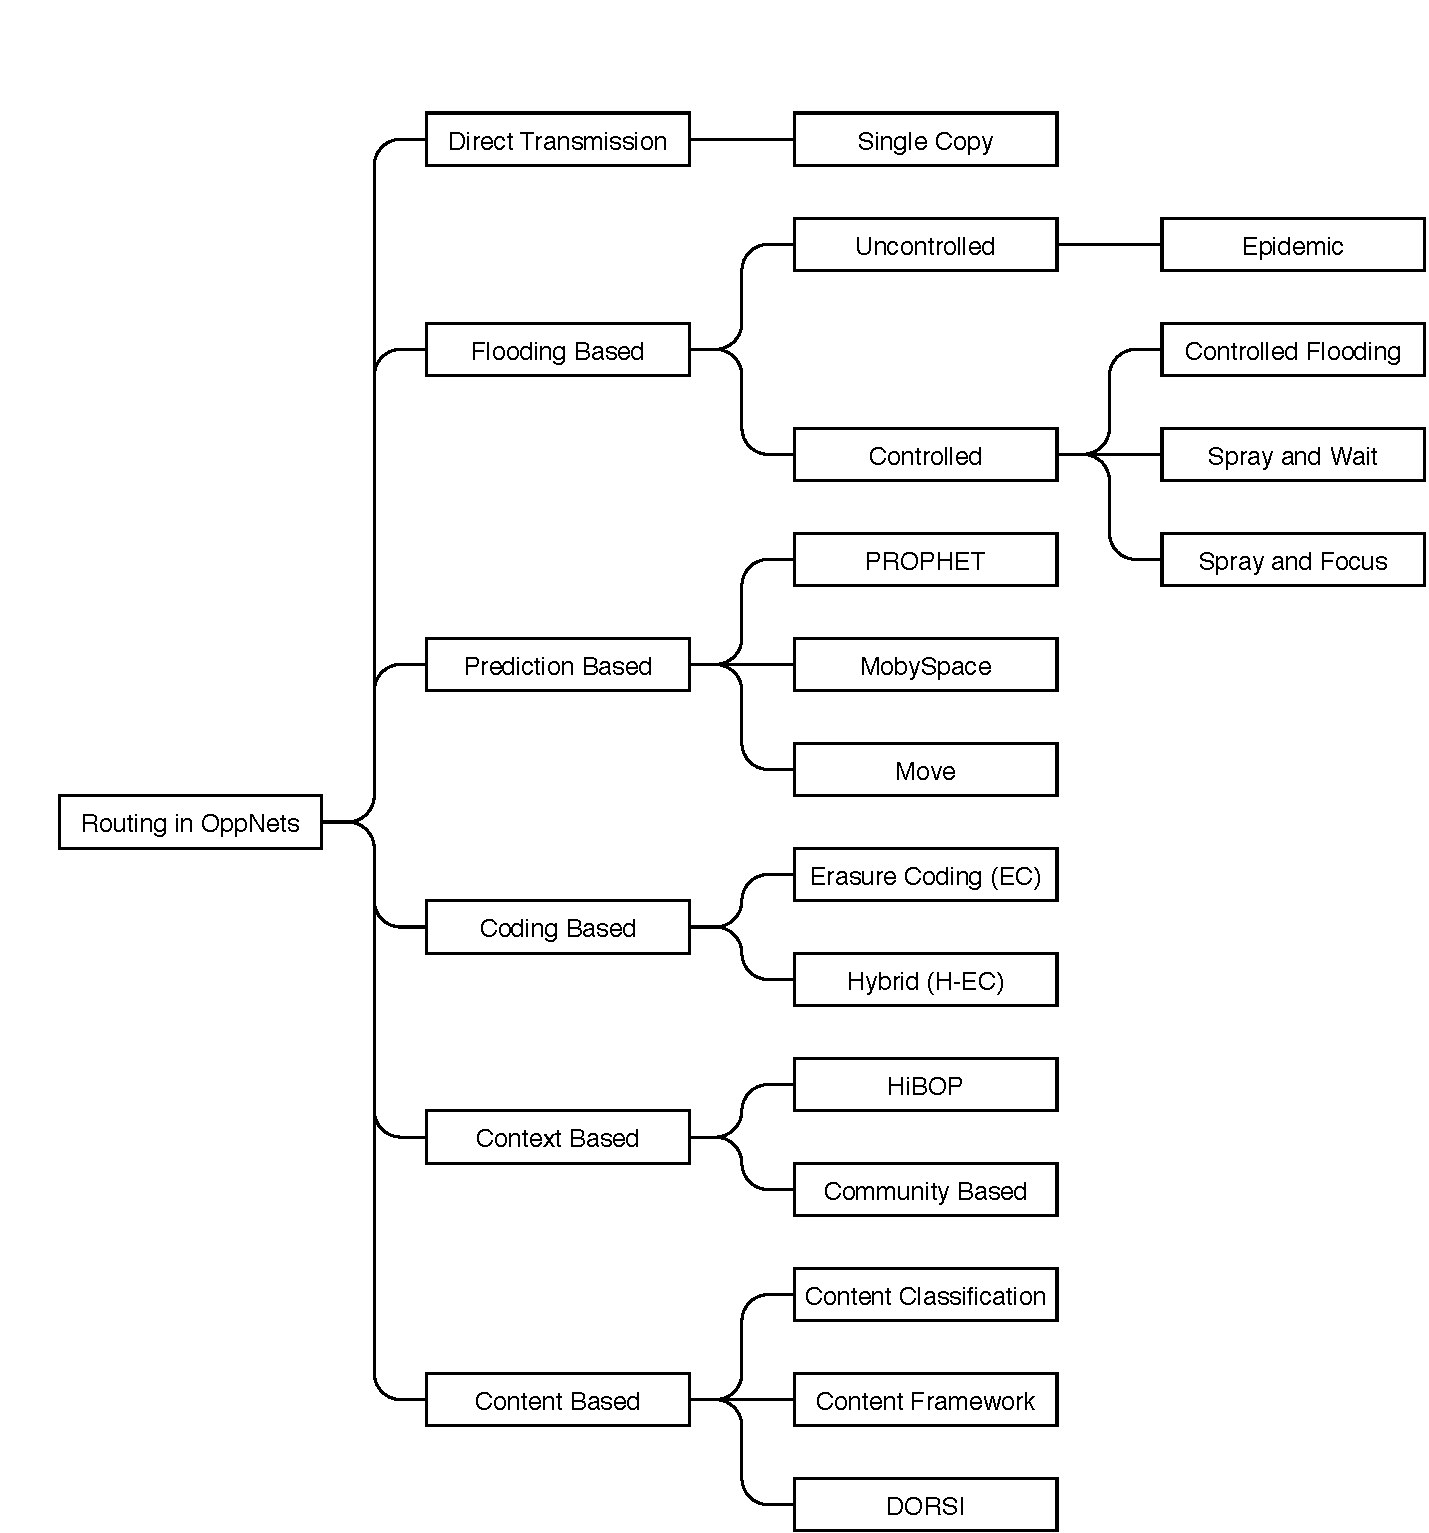
\includegraphics[width=1.0\columnwidth]{Figures/RoutingInOppNets.pdf}
% 	\caption{Classification of Opportunistic Routing}
% 	\label{fig:bg:RoutingInOppNets}
% \end{figure}

%% This part is folding for OppNet routing diagram
\begin{figure}
	\centering
% Graphic for TeX using PGF
% Title: /Users/Arm/Desktop/Diagram1.dia
% Creator: Dia v0.97.2
% CreationDate: Fri Sep 12 16:02:14 2014
% For: Arm
% \usepackage{tikz}
% The following commands are not supported in PSTricks at present
% We define them conditionally, so when they are implemented,
% this pgf file will use them.
\ifx\du\undefined
  \newlength{\du}
\fi
\setlength{\du}{15\unitlength}
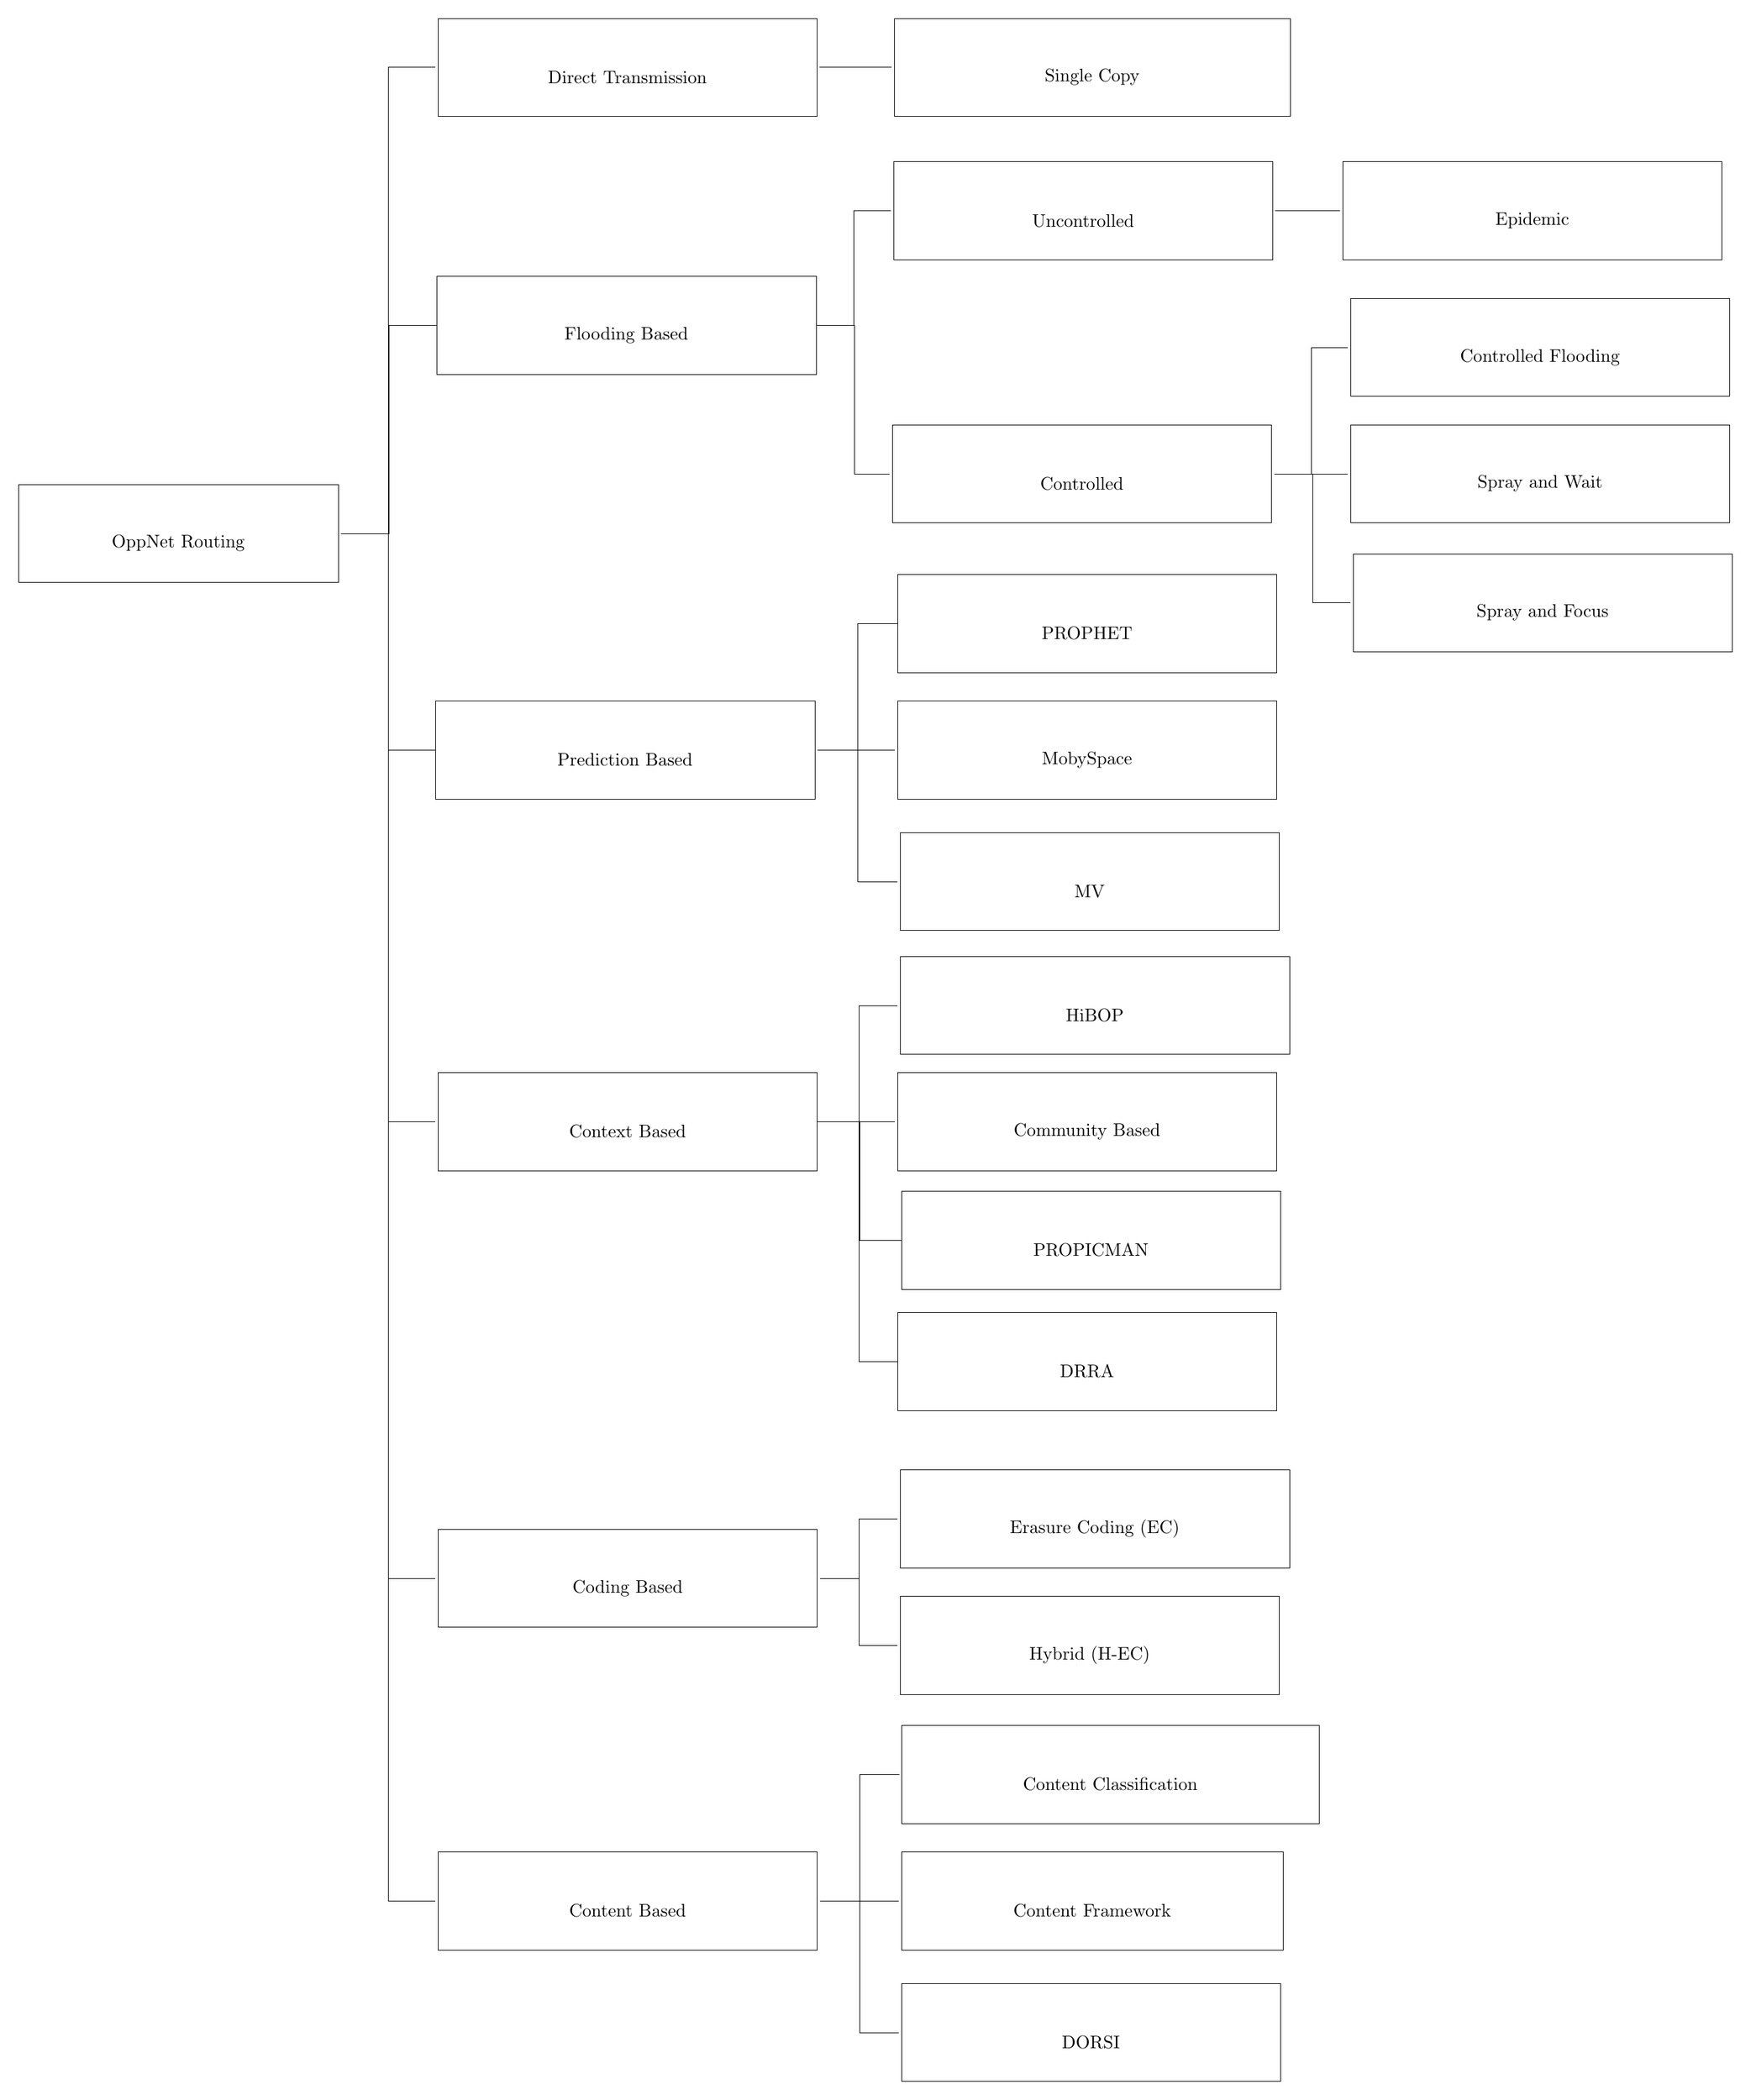
\begin{tikzpicture}
\pgftransformxscale{1.000000}
\pgftransformyscale{-1.000000}
\definecolor{dialinecolor}{rgb}{0.000000, 0.000000, 0.000000}
\pgfsetstrokecolor{dialinecolor}
\definecolor{dialinecolor}{rgb}{1.000000, 1.000000, 1.000000}
\pgfsetfillcolor{dialinecolor}
\definecolor{dialinecolor}{rgb}{1.000000, 1.000000, 1.000000}
\pgfsetfillcolor{dialinecolor}
\fill (3.606250\du,23.050000\du)--(3.606250\du,24.950000\du)--(9.808750\du,24.950000\du)--(9.808750\du,23.050000\du)--cycle;
\pgfsetlinewidth{0.100000\du}
\pgfsetdash{}{0pt}
\pgfsetdash{}{0pt}
\pgfsetmiterjoin
\definecolor{dialinecolor}{rgb}{0.000000, 0.000000, 0.000000}
\pgfsetstrokecolor{dialinecolor}
\draw (3.606250\du,23.050000\du)--(3.606250\du,24.950000\du)--(9.808750\du,24.950000\du)--(9.808750\du,23.050000\du)--cycle;
% setfont left to latex
\definecolor{dialinecolor}{rgb}{0.000000, 0.000000, 0.000000}
\pgfsetstrokecolor{dialinecolor}
\node at (6.707500\du,24.195000\du){OppNet Routing};
\definecolor{dialinecolor}{rgb}{1.000000, 1.000000, 1.000000}
\pgfsetfillcolor{dialinecolor}
\fill (11.736200\du,14.020000\du)--(11.736200\du,15.920000\du)--(19.081200\du,15.920000\du)--(19.081200\du,14.020000\du)--cycle;
\pgfsetlinewidth{0.100000\du}
\pgfsetdash{}{0pt}
\pgfsetdash{}{0pt}
\pgfsetmiterjoin
\definecolor{dialinecolor}{rgb}{0.000000, 0.000000, 0.000000}
\pgfsetstrokecolor{dialinecolor}
\draw (11.736200\du,14.020000\du)--(11.736200\du,15.920000\du)--(19.081200\du,15.920000\du)--(19.081200\du,14.020000\du)--cycle;
% setfont left to latex
\definecolor{dialinecolor}{rgb}{0.000000, 0.000000, 0.000000}
\pgfsetstrokecolor{dialinecolor}
\node at (15.408700\du,15.165000\du){Direct Transmission};
\pgfsetlinewidth{0.100000\du}
\pgfsetdash{}{0pt}
\pgfsetdash{}{0pt}
\pgfsetmiterjoin
\pgfsetbuttcap
{
\definecolor{dialinecolor}{rgb}{0.000000, 0.000000, 0.000000}
\pgfsetfillcolor{dialinecolor}
% was here!!!
{\pgfsetcornersarced{\pgfpoint{0.000000\du}{0.000000\du}}\definecolor{dialinecolor}{rgb}{0.000000, 0.000000, 0.000000}
\pgfsetstrokecolor{dialinecolor}
\draw (9.859135\du,24.000000\du)--(10.772440\du,24.000000\du)--(10.772440\du,14.970000\du)--(11.685746\du,14.970000\du);
}}
\definecolor{dialinecolor}{rgb}{1.000000, 1.000000, 1.000000}
\pgfsetfillcolor{dialinecolor}
\fill (20.574100\du,14.020000\du)--(20.574100\du,15.920000\du)--(28.250804\du,15.920000\du)--(28.250804\du,14.020000\du)--cycle;
\pgfsetlinewidth{0.100000\du}
\pgfsetdash{}{0pt}
\pgfsetdash{}{0pt}
\pgfsetmiterjoin
\definecolor{dialinecolor}{rgb}{0.000000, 0.000000, 0.000000}
\pgfsetstrokecolor{dialinecolor}
\draw (20.574100\du,14.020000\du)--(20.574100\du,15.920000\du)--(28.250804\du,15.920000\du)--(28.250804\du,14.020000\du)--cycle;
% setfont left to latex
\definecolor{dialinecolor}{rgb}{0.000000, 0.000000, 0.000000}
\pgfsetstrokecolor{dialinecolor}
\node at (24.412452\du,15.165000\du){Single Copy};
\pgfsetlinewidth{0.100000\du}
\pgfsetdash{}{0pt}
\pgfsetdash{}{0pt}
\pgfsetmiterjoin
\pgfsetbuttcap
{
\definecolor{dialinecolor}{rgb}{0.000000, 0.000000, 0.000000}
\pgfsetfillcolor{dialinecolor}
% was here!!!
{\pgfsetcornersarced{\pgfpoint{0.000000\du}{0.000000\du}}\definecolor{dialinecolor}{rgb}{0.000000, 0.000000, 0.000000}
\pgfsetstrokecolor{dialinecolor}
\draw (19.131654\du,14.970000\du)--(19.181654\du,14.970000\du)--(20.473625\du,14.970000\du)--(20.523625\du,14.970000\du);
}}
\definecolor{dialinecolor}{rgb}{1.000000, 1.000000, 1.000000}
\pgfsetfillcolor{dialinecolor}
\fill (11.715000\du,19.020000\du)--(11.715000\du,20.920000\du)--(19.060000\du,20.920000\du)--(19.060000\du,19.020000\du)--cycle;
\pgfsetlinewidth{0.100000\du}
\pgfsetdash{}{0pt}
\pgfsetdash{}{0pt}
\pgfsetmiterjoin
\definecolor{dialinecolor}{rgb}{0.000000, 0.000000, 0.000000}
\pgfsetstrokecolor{dialinecolor}
\draw (11.715000\du,19.020000\du)--(11.715000\du,20.920000\du)--(19.060000\du,20.920000\du)--(19.060000\du,19.020000\du)--cycle;
% setfont left to latex
\definecolor{dialinecolor}{rgb}{0.000000, 0.000000, 0.000000}
\pgfsetstrokecolor{dialinecolor}
\node at (15.387500\du,20.165000\du){Flooding Based};
\definecolor{dialinecolor}{rgb}{1.000000, 1.000000, 1.000000}
\pgfsetfillcolor{dialinecolor}
\fill (20.565000\du,16.795000\du)--(20.565000\du,18.695000\du)--(27.910000\du,18.695000\du)--(27.910000\du,16.795000\du)--cycle;
\pgfsetlinewidth{0.100000\du}
\pgfsetdash{}{0pt}
\pgfsetdash{}{0pt}
\pgfsetmiterjoin
\definecolor{dialinecolor}{rgb}{0.000000, 0.000000, 0.000000}
\pgfsetstrokecolor{dialinecolor}
\draw (20.565000\du,16.795000\du)--(20.565000\du,18.695000\du)--(27.910000\du,18.695000\du)--(27.910000\du,16.795000\du)--cycle;
% setfont left to latex
\definecolor{dialinecolor}{rgb}{0.000000, 0.000000, 0.000000}
\pgfsetstrokecolor{dialinecolor}
\node at (24.237500\du,17.940000\du){Uncontrolled};
\definecolor{dialinecolor}{rgb}{1.000000, 1.000000, 1.000000}
\pgfsetfillcolor{dialinecolor}
\fill (20.540000\du,21.895000\du)--(20.540000\du,23.795000\du)--(27.885000\du,23.795000\du)--(27.885000\du,21.895000\du)--cycle;
\pgfsetlinewidth{0.100000\du}
\pgfsetdash{}{0pt}
\pgfsetdash{}{0pt}
\pgfsetmiterjoin
\definecolor{dialinecolor}{rgb}{0.000000, 0.000000, 0.000000}
\pgfsetstrokecolor{dialinecolor}
\draw (20.540000\du,21.895000\du)--(20.540000\du,23.795000\du)--(27.885000\du,23.795000\du)--(27.885000\du,21.895000\du)--cycle;
% setfont left to latex
\definecolor{dialinecolor}{rgb}{0.000000, 0.000000, 0.000000}
\pgfsetstrokecolor{dialinecolor}
\node at (24.212500\du,23.040000\du){Controlled};
\definecolor{dialinecolor}{rgb}{1.000000, 1.000000, 1.000000}
\pgfsetfillcolor{dialinecolor}
\fill (29.265000\du,16.795000\du)--(29.265000\du,18.695000\du)--(36.610000\du,18.695000\du)--(36.610000\du,16.795000\du)--cycle;
\pgfsetlinewidth{0.100000\du}
\pgfsetdash{}{0pt}
\pgfsetdash{}{0pt}
\pgfsetmiterjoin
\definecolor{dialinecolor}{rgb}{0.000000, 0.000000, 0.000000}
\pgfsetstrokecolor{dialinecolor}
\draw (29.265000\du,16.795000\du)--(29.265000\du,18.695000\du)--(36.610000\du,18.695000\du)--(36.610000\du,16.795000\du)--cycle;
% setfont left to latex
\definecolor{dialinecolor}{rgb}{0.000000, 0.000000, 0.000000}
\pgfsetstrokecolor{dialinecolor}
\node at (32.937500\du,17.940000\du){Epidemic};
\pgfsetlinewidth{0.100000\du}
\pgfsetdash{}{0pt}
\pgfsetdash{}{0pt}
\pgfsetmiterjoin
\pgfsetbuttcap
{
\definecolor{dialinecolor}{rgb}{0.000000, 0.000000, 0.000000}
\pgfsetfillcolor{dialinecolor}
% was here!!!
{\pgfsetcornersarced{\pgfpoint{0.000000\du}{0.000000\du}}\definecolor{dialinecolor}{rgb}{0.000000, 0.000000, 0.000000}
\pgfsetstrokecolor{dialinecolor}
\draw (9.859135\du,24.000000\du)--(10.787067\du,24.000000\du)--(10.787067\du,19.970000\du)--(11.715000\du,19.970000\du);
}}
\pgfsetlinewidth{0.100000\du}
\pgfsetdash{}{0pt}
\pgfsetdash{}{0pt}
\pgfsetmiterjoin
\pgfsetbuttcap
{
\definecolor{dialinecolor}{rgb}{0.000000, 0.000000, 0.000000}
\pgfsetfillcolor{dialinecolor}
% was here!!!
{\pgfsetcornersarced{\pgfpoint{0.000000\du}{0.000000\du}}\definecolor{dialinecolor}{rgb}{0.000000, 0.000000, 0.000000}
\pgfsetstrokecolor{dialinecolor}
\draw (19.060000\du,19.970000\du)--(19.787273\du,19.970000\du)--(19.787273\du,17.745000\du)--(20.514546\du,17.745000\du);
}}
\pgfsetlinewidth{0.100000\du}
\pgfsetdash{}{0pt}
\pgfsetdash{}{0pt}
\pgfsetmiterjoin
\pgfsetbuttcap
{
\definecolor{dialinecolor}{rgb}{0.000000, 0.000000, 0.000000}
\pgfsetfillcolor{dialinecolor}
% was here!!!
{\pgfsetcornersarced{\pgfpoint{0.000000\du}{0.000000\du}}\definecolor{dialinecolor}{rgb}{0.000000, 0.000000, 0.000000}
\pgfsetstrokecolor{dialinecolor}
\draw (19.110454\du,19.970000\du)--(19.800000\du,19.970000\du)--(19.800000\du,22.845000\du)--(20.489546\du,22.845000\du);
}}
\pgfsetlinewidth{0.100000\du}
\pgfsetdash{}{0pt}
\pgfsetdash{}{0pt}
\pgfsetmiterjoin
\pgfsetbuttcap
{
\definecolor{dialinecolor}{rgb}{0.000000, 0.000000, 0.000000}
\pgfsetfillcolor{dialinecolor}
% was here!!!
{\pgfsetcornersarced{\pgfpoint{0.000000\du}{0.000000\du}}\definecolor{dialinecolor}{rgb}{0.000000, 0.000000, 0.000000}
\pgfsetstrokecolor{dialinecolor}
\draw (27.960454\du,17.745000\du)--(28.010454\du,17.745000\du)--(29.164546\du,17.745000\du)--(29.214546\du,17.745000\du);
}}
\definecolor{dialinecolor}{rgb}{1.000000, 1.000000, 1.000000}
\pgfsetfillcolor{dialinecolor}
\fill (29.415000\du,19.445000\du)--(29.415000\du,21.345000\du)--(36.760000\du,21.345000\du)--(36.760000\du,19.445000\du)--cycle;
\pgfsetlinewidth{0.100000\du}
\pgfsetdash{}{0pt}
\pgfsetdash{}{0pt}
\pgfsetmiterjoin
\definecolor{dialinecolor}{rgb}{0.000000, 0.000000, 0.000000}
\pgfsetstrokecolor{dialinecolor}
\draw (29.415000\du,19.445000\du)--(29.415000\du,21.345000\du)--(36.760000\du,21.345000\du)--(36.760000\du,19.445000\du)--cycle;
% setfont left to latex
\definecolor{dialinecolor}{rgb}{0.000000, 0.000000, 0.000000}
\pgfsetstrokecolor{dialinecolor}
\node at (33.087500\du,20.590000\du){Controlled Flooding};
\definecolor{dialinecolor}{rgb}{1.000000, 1.000000, 1.000000}
\pgfsetfillcolor{dialinecolor}
\fill (29.415000\du,21.895000\du)--(29.415000\du,23.795000\du)--(36.760000\du,23.795000\du)--(36.760000\du,21.895000\du)--cycle;
\pgfsetlinewidth{0.100000\du}
\pgfsetdash{}{0pt}
\pgfsetdash{}{0pt}
\pgfsetmiterjoin
\definecolor{dialinecolor}{rgb}{0.000000, 0.000000, 0.000000}
\pgfsetstrokecolor{dialinecolor}
\draw (29.415000\du,21.895000\du)--(29.415000\du,23.795000\du)--(36.760000\du,23.795000\du)--(36.760000\du,21.895000\du)--cycle;
% setfont left to latex
\definecolor{dialinecolor}{rgb}{0.000000, 0.000000, 0.000000}
\pgfsetstrokecolor{dialinecolor}
\node at (33.087500\du,23.040000\du){Spray and Wait};
\definecolor{dialinecolor}{rgb}{1.000000, 1.000000, 1.000000}
\pgfsetfillcolor{dialinecolor}
\fill (29.465000\du,24.395000\du)--(29.465000\du,26.295000\du)--(36.810000\du,26.295000\du)--(36.810000\du,24.395000\du)--cycle;
\pgfsetlinewidth{0.100000\du}
\pgfsetdash{}{0pt}
\pgfsetdash{}{0pt}
\pgfsetmiterjoin
\definecolor{dialinecolor}{rgb}{0.000000, 0.000000, 0.000000}
\pgfsetstrokecolor{dialinecolor}
\draw (29.465000\du,24.395000\du)--(29.465000\du,26.295000\du)--(36.810000\du,26.295000\du)--(36.810000\du,24.395000\du)--cycle;
% setfont left to latex
\definecolor{dialinecolor}{rgb}{0.000000, 0.000000, 0.000000}
\pgfsetstrokecolor{dialinecolor}
\node at (33.137500\du,25.540000\du){Spray and Focus};
\pgfsetlinewidth{0.100000\du}
\pgfsetdash{}{0pt}
\pgfsetdash{}{0pt}
\pgfsetmiterjoin
\pgfsetbuttcap
{
\definecolor{dialinecolor}{rgb}{0.000000, 0.000000, 0.000000}
\pgfsetfillcolor{dialinecolor}
% was here!!!
{\pgfsetcornersarced{\pgfpoint{0.000000\du}{0.000000\du}}\definecolor{dialinecolor}{rgb}{0.000000, 0.000000, 0.000000}
\pgfsetstrokecolor{dialinecolor}
\draw (27.935454\du,22.845000\du)--(28.650000\du,22.845000\du)--(28.650000\du,20.395000\du)--(29.364546\du,20.395000\du);
}}
\pgfsetlinewidth{0.100000\du}
\pgfsetdash{}{0pt}
\pgfsetdash{}{0pt}
\pgfsetmiterjoin
\pgfsetbuttcap
{
\definecolor{dialinecolor}{rgb}{0.000000, 0.000000, 0.000000}
\pgfsetfillcolor{dialinecolor}
% was here!!!
{\pgfsetcornersarced{\pgfpoint{0.000000\du}{0.000000\du}}\definecolor{dialinecolor}{rgb}{0.000000, 0.000000, 0.000000}
\pgfsetstrokecolor{dialinecolor}
\draw (27.935454\du,22.845000\du)--(27.985454\du,22.845000\du)--(29.314546\du,22.845000\du)--(29.364546\du,22.845000\du);
}}
\pgfsetlinewidth{0.100000\du}
\pgfsetdash{}{0pt}
\pgfsetdash{}{0pt}
\pgfsetmiterjoin
\pgfsetbuttcap
{
\definecolor{dialinecolor}{rgb}{0.000000, 0.000000, 0.000000}
\pgfsetfillcolor{dialinecolor}
% was here!!!
{\pgfsetcornersarced{\pgfpoint{0.000000\du}{0.000000\du}}\definecolor{dialinecolor}{rgb}{0.000000, 0.000000, 0.000000}
\pgfsetstrokecolor{dialinecolor}
\draw (27.935454\du,22.845000\du)--(28.675000\du,22.845000\du)--(28.675000\du,25.345000\du)--(29.414546\du,25.345000\du);
}}
\definecolor{dialinecolor}{rgb}{1.000000, 1.000000, 1.000000}
\pgfsetfillcolor{dialinecolor}
\fill (11.690000\du,27.245000\du)--(11.690000\du,29.145000\du)--(19.035000\du,29.145000\du)--(19.035000\du,27.245000\du)--cycle;
\pgfsetlinewidth{0.100000\du}
\pgfsetdash{}{0pt}
\pgfsetdash{}{0pt}
\pgfsetmiterjoin
\definecolor{dialinecolor}{rgb}{0.000000, 0.000000, 0.000000}
\pgfsetstrokecolor{dialinecolor}
\draw (11.690000\du,27.245000\du)--(11.690000\du,29.145000\du)--(19.035000\du,29.145000\du)--(19.035000\du,27.245000\du)--cycle;
% setfont left to latex
\definecolor{dialinecolor}{rgb}{0.000000, 0.000000, 0.000000}
\pgfsetstrokecolor{dialinecolor}
\node at (15.362500\du,28.390000\du){Prediction Based};
\definecolor{dialinecolor}{rgb}{1.000000, 1.000000, 1.000000}
\pgfsetfillcolor{dialinecolor}
\fill (20.640000\du,24.795000\du)--(20.640000\du,26.695000\du)--(27.985000\du,26.695000\du)--(27.985000\du,24.795000\du)--cycle;
\pgfsetlinewidth{0.100000\du}
\pgfsetdash{}{0pt}
\pgfsetdash{}{0pt}
\pgfsetmiterjoin
\definecolor{dialinecolor}{rgb}{0.000000, 0.000000, 0.000000}
\pgfsetstrokecolor{dialinecolor}
\draw (20.640000\du,24.795000\du)--(20.640000\du,26.695000\du)--(27.985000\du,26.695000\du)--(27.985000\du,24.795000\du)--cycle;
% setfont left to latex
\definecolor{dialinecolor}{rgb}{0.000000, 0.000000, 0.000000}
\pgfsetstrokecolor{dialinecolor}
\node at (24.312500\du,25.940000\du){PROPHET};
\definecolor{dialinecolor}{rgb}{1.000000, 1.000000, 1.000000}
\pgfsetfillcolor{dialinecolor}
\fill (20.640000\du,27.245000\du)--(20.640000\du,29.145000\du)--(27.985000\du,29.145000\du)--(27.985000\du,27.245000\du)--cycle;
\pgfsetlinewidth{0.100000\du}
\pgfsetdash{}{0pt}
\pgfsetdash{}{0pt}
\pgfsetmiterjoin
\definecolor{dialinecolor}{rgb}{0.000000, 0.000000, 0.000000}
\pgfsetstrokecolor{dialinecolor}
\draw (20.640000\du,27.245000\du)--(20.640000\du,29.145000\du)--(27.985000\du,29.145000\du)--(27.985000\du,27.245000\du)--cycle;
% setfont left to latex
\definecolor{dialinecolor}{rgb}{0.000000, 0.000000, 0.000000}
\pgfsetstrokecolor{dialinecolor}
\node at (24.312500\du,28.390000\du){MobySpace};
\definecolor{dialinecolor}{rgb}{1.000000, 1.000000, 1.000000}
\pgfsetfillcolor{dialinecolor}
\fill (20.690000\du,29.795000\du)--(20.690000\du,31.695000\du)--(28.035000\du,31.695000\du)--(28.035000\du,29.795000\du)--cycle;
\pgfsetlinewidth{0.100000\du}
\pgfsetdash{}{0pt}
\pgfsetdash{}{0pt}
\pgfsetmiterjoin
\definecolor{dialinecolor}{rgb}{0.000000, 0.000000, 0.000000}
\pgfsetstrokecolor{dialinecolor}
\draw (20.690000\du,29.795000\du)--(20.690000\du,31.695000\du)--(28.035000\du,31.695000\du)--(28.035000\du,29.795000\du)--cycle;
% setfont left to latex
\definecolor{dialinecolor}{rgb}{0.000000, 0.000000, 0.000000}
\pgfsetstrokecolor{dialinecolor}
\node at (24.362500\du,30.940000\du){MV};
\pgfsetlinewidth{0.100000\du}
\pgfsetdash{}{0pt}
\pgfsetdash{}{0pt}
\pgfsetmiterjoin
\pgfsetbuttcap
{
\definecolor{dialinecolor}{rgb}{0.000000, 0.000000, 0.000000}
\pgfsetfillcolor{dialinecolor}
% was here!!!
{\pgfsetcornersarced{\pgfpoint{0.000000\du}{0.000000\du}}\definecolor{dialinecolor}{rgb}{0.000000, 0.000000, 0.000000}
\pgfsetstrokecolor{dialinecolor}
\draw (9.859135\du,24.000000\du)--(10.774567\du,24.000000\du)--(10.774567\du,28.195000\du)--(11.690000\du,28.195000\du);
}}
\pgfsetlinewidth{0.100000\du}
\pgfsetdash{}{0pt}
\pgfsetdash{}{0pt}
\pgfsetmiterjoin
\pgfsetbuttcap
{
\definecolor{dialinecolor}{rgb}{0.000000, 0.000000, 0.000000}
\pgfsetfillcolor{dialinecolor}
% was here!!!
{\pgfsetcornersarced{\pgfpoint{0.000000\du}{0.000000\du}}\definecolor{dialinecolor}{rgb}{0.000000, 0.000000, 0.000000}
\pgfsetstrokecolor{dialinecolor}
\draw (19.085454\du,28.195000\du)--(19.862727\du,28.195000\du)--(19.862727\du,25.745000\du)--(20.640000\du,25.745000\du);
}}
\pgfsetlinewidth{0.100000\du}
\pgfsetdash{}{0pt}
\pgfsetdash{}{0pt}
\pgfsetmiterjoin
\pgfsetbuttcap
{
\definecolor{dialinecolor}{rgb}{0.000000, 0.000000, 0.000000}
\pgfsetfillcolor{dialinecolor}
% was here!!!
{\pgfsetcornersarced{\pgfpoint{0.000000\du}{0.000000\du}}\definecolor{dialinecolor}{rgb}{0.000000, 0.000000, 0.000000}
\pgfsetstrokecolor{dialinecolor}
\draw (19.085454\du,28.195000\du)--(19.135454\du,28.195000\du)--(20.539546\du,28.195000\du)--(20.589546\du,28.195000\du);
}}
\pgfsetlinewidth{0.100000\du}
\pgfsetdash{}{0pt}
\pgfsetdash{}{0pt}
\pgfsetmiterjoin
\pgfsetbuttcap
{
\definecolor{dialinecolor}{rgb}{0.000000, 0.000000, 0.000000}
\pgfsetfillcolor{dialinecolor}
% was here!!!
{\pgfsetcornersarced{\pgfpoint{0.000000\du}{0.000000\du}}\definecolor{dialinecolor}{rgb}{0.000000, 0.000000, 0.000000}
\pgfsetstrokecolor{dialinecolor}
\draw (19.085454\du,28.195000\du)--(19.862500\du,28.195000\du)--(19.862500\du,30.745000\du)--(20.639546\du,30.745000\du);
}}
\definecolor{dialinecolor}{rgb}{1.000000, 1.000000, 1.000000}
\pgfsetfillcolor{dialinecolor}
\fill (11.740000\du,43.295000\du)--(11.740000\du,45.195000\du)--(19.085000\du,45.195000\du)--(19.085000\du,43.295000\du)--cycle;
\pgfsetlinewidth{0.100000\du}
\pgfsetdash{}{0pt}
\pgfsetdash{}{0pt}
\pgfsetmiterjoin
\definecolor{dialinecolor}{rgb}{0.000000, 0.000000, 0.000000}
\pgfsetstrokecolor{dialinecolor}
\draw (11.740000\du,43.295000\du)--(11.740000\du,45.195000\du)--(19.085000\du,45.195000\du)--(19.085000\du,43.295000\du)--cycle;
% setfont left to latex
\definecolor{dialinecolor}{rgb}{0.000000, 0.000000, 0.000000}
\pgfsetstrokecolor{dialinecolor}
\node at (15.412500\du,44.440000\du){Coding Based};
\definecolor{dialinecolor}{rgb}{1.000000, 1.000000, 1.000000}
\pgfsetfillcolor{dialinecolor}
\fill (20.695000\du,42.145000\du)--(20.695000\du,44.045000\du)--(28.230000\du,44.045000\du)--(28.230000\du,42.145000\du)--cycle;
\pgfsetlinewidth{0.100000\du}
\pgfsetdash{}{0pt}
\pgfsetdash{}{0pt}
\pgfsetmiterjoin
\definecolor{dialinecolor}{rgb}{0.000000, 0.000000, 0.000000}
\pgfsetstrokecolor{dialinecolor}
\draw (20.695000\du,42.145000\du)--(20.695000\du,44.045000\du)--(28.230000\du,44.045000\du)--(28.230000\du,42.145000\du)--cycle;
% setfont left to latex
\definecolor{dialinecolor}{rgb}{0.000000, 0.000000, 0.000000}
\pgfsetstrokecolor{dialinecolor}
\node at (24.462500\du,43.290000\du){Erasure Coding (EC)};
\definecolor{dialinecolor}{rgb}{1.000000, 1.000000, 1.000000}
\pgfsetfillcolor{dialinecolor}
\fill (20.690000\du,44.595000\du)--(20.690000\du,46.495000\du)--(28.035000\du,46.495000\du)--(28.035000\du,44.595000\du)--cycle;
\pgfsetlinewidth{0.100000\du}
\pgfsetdash{}{0pt}
\pgfsetdash{}{0pt}
\pgfsetmiterjoin
\definecolor{dialinecolor}{rgb}{0.000000, 0.000000, 0.000000}
\pgfsetstrokecolor{dialinecolor}
\draw (20.690000\du,44.595000\du)--(20.690000\du,46.495000\du)--(28.035000\du,46.495000\du)--(28.035000\du,44.595000\du)--cycle;
% setfont left to latex
\definecolor{dialinecolor}{rgb}{0.000000, 0.000000, 0.000000}
\pgfsetstrokecolor{dialinecolor}
\node at (24.362500\du,45.740000\du){Hybrid (H-EC)};
\pgfsetlinewidth{0.100000\du}
\pgfsetdash{}{0pt}
\pgfsetdash{}{0pt}
\pgfsetmiterjoin
\pgfsetbuttcap
{
\definecolor{dialinecolor}{rgb}{0.000000, 0.000000, 0.000000}
\pgfsetfillcolor{dialinecolor}
% was here!!!
{\pgfsetcornersarced{\pgfpoint{0.000000\du}{0.000000\du}}\definecolor{dialinecolor}{rgb}{0.000000, 0.000000, 0.000000}
\pgfsetstrokecolor{dialinecolor}
\draw (9.859135\du,24.000000\du)--(10.774340\du,24.000000\du)--(10.774340\du,44.245000\du)--(11.689546\du,44.245000\du);
}}
\pgfsetlinewidth{0.100000\du}
\pgfsetdash{}{0pt}
\pgfsetdash{}{0pt}
\pgfsetmiterjoin
\pgfsetbuttcap
{
\definecolor{dialinecolor}{rgb}{0.000000, 0.000000, 0.000000}
\pgfsetfillcolor{dialinecolor}
% was here!!!
{\pgfsetcornersarced{\pgfpoint{0.000000\du}{0.000000\du}}\definecolor{dialinecolor}{rgb}{0.000000, 0.000000, 0.000000}
\pgfsetstrokecolor{dialinecolor}
\draw (19.135454\du,44.245000\du)--(19.889994\du,44.245000\du)--(19.889994\du,43.095000\du)--(20.644534\du,43.095000\du);
}}
\pgfsetlinewidth{0.100000\du}
\pgfsetdash{}{0pt}
\pgfsetdash{}{0pt}
\pgfsetmiterjoin
\pgfsetbuttcap
{
\definecolor{dialinecolor}{rgb}{0.000000, 0.000000, 0.000000}
\pgfsetfillcolor{dialinecolor}
% was here!!!
{\pgfsetcornersarced{\pgfpoint{0.000000\du}{0.000000\du}}\definecolor{dialinecolor}{rgb}{0.000000, 0.000000, 0.000000}
\pgfsetstrokecolor{dialinecolor}
\draw (19.135454\du,44.245000\du)--(19.887500\du,44.245000\du)--(19.887500\du,45.545000\du)--(20.639546\du,45.545000\du);
}}
\definecolor{dialinecolor}{rgb}{1.000000, 1.000000, 1.000000}
\pgfsetfillcolor{dialinecolor}
\fill (11.740000\du,34.445000\du)--(11.740000\du,36.345000\du)--(19.085000\du,36.345000\du)--(19.085000\du,34.445000\du)--cycle;
\pgfsetlinewidth{0.100000\du}
\pgfsetdash{}{0pt}
\pgfsetdash{}{0pt}
\pgfsetmiterjoin
\definecolor{dialinecolor}{rgb}{0.000000, 0.000000, 0.000000}
\pgfsetstrokecolor{dialinecolor}
\draw (11.740000\du,34.445000\du)--(11.740000\du,36.345000\du)--(19.085000\du,36.345000\du)--(19.085000\du,34.445000\du)--cycle;
% setfont left to latex
\definecolor{dialinecolor}{rgb}{0.000000, 0.000000, 0.000000}
\pgfsetstrokecolor{dialinecolor}
\node at (15.412500\du,35.590000\du){Context Based};
\definecolor{dialinecolor}{rgb}{1.000000, 1.000000, 1.000000}
\pgfsetfillcolor{dialinecolor}
\fill (20.695000\du,32.195000\du)--(20.695000\du,34.095000\du)--(28.230000\du,34.095000\du)--(28.230000\du,32.195000\du)--cycle;
\pgfsetlinewidth{0.100000\du}
\pgfsetdash{}{0pt}
\pgfsetdash{}{0pt}
\pgfsetmiterjoin
\definecolor{dialinecolor}{rgb}{0.000000, 0.000000, 0.000000}
\pgfsetstrokecolor{dialinecolor}
\draw (20.695000\du,32.195000\du)--(20.695000\du,34.095000\du)--(28.230000\du,34.095000\du)--(28.230000\du,32.195000\du)--cycle;
% setfont left to latex
\definecolor{dialinecolor}{rgb}{0.000000, 0.000000, 0.000000}
\pgfsetstrokecolor{dialinecolor}
\node at (24.462500\du,33.340000\du){HiBOP};
\definecolor{dialinecolor}{rgb}{1.000000, 1.000000, 1.000000}
\pgfsetfillcolor{dialinecolor}
\fill (20.640000\du,34.445000\du)--(20.640000\du,36.345000\du)--(27.985000\du,36.345000\du)--(27.985000\du,34.445000\du)--cycle;
\pgfsetlinewidth{0.100000\du}
\pgfsetdash{}{0pt}
\pgfsetdash{}{0pt}
\pgfsetmiterjoin
\definecolor{dialinecolor}{rgb}{0.000000, 0.000000, 0.000000}
\pgfsetstrokecolor{dialinecolor}
\draw (20.640000\du,34.445000\du)--(20.640000\du,36.345000\du)--(27.985000\du,36.345000\du)--(27.985000\du,34.445000\du)--cycle;
% setfont left to latex
\definecolor{dialinecolor}{rgb}{0.000000, 0.000000, 0.000000}
\pgfsetstrokecolor{dialinecolor}
\node at (24.312500\du,35.590000\du){Community Based};
\pgfsetlinewidth{0.100000\du}
\pgfsetdash{}{0pt}
\pgfsetdash{}{0pt}
\pgfsetmiterjoin
\pgfsetbuttcap
{
\definecolor{dialinecolor}{rgb}{0.000000, 0.000000, 0.000000}
\pgfsetfillcolor{dialinecolor}
% was here!!!
{\pgfsetcornersarced{\pgfpoint{0.000000\du}{0.000000\du}}\definecolor{dialinecolor}{rgb}{0.000000, 0.000000, 0.000000}
\pgfsetstrokecolor{dialinecolor}
\draw (9.859135\du,24.000000\du)--(10.774340\du,24.000000\du)--(10.774340\du,35.395000\du)--(11.689546\du,35.395000\du);
}}
\pgfsetlinewidth{0.100000\du}
\pgfsetdash{}{0pt}
\pgfsetdash{}{0pt}
\pgfsetmiterjoin
\pgfsetbuttcap
{
\definecolor{dialinecolor}{rgb}{0.000000, 0.000000, 0.000000}
\pgfsetfillcolor{dialinecolor}
% was here!!!
{\pgfsetcornersarced{\pgfpoint{0.000000\du}{0.000000\du}}\definecolor{dialinecolor}{rgb}{0.000000, 0.000000, 0.000000}
\pgfsetstrokecolor{dialinecolor}
\draw (19.135454\du,35.395000\du)--(19.889994\du,35.395000\du)--(19.889994\du,33.145000\du)--(20.644534\du,33.145000\du);
}}
\pgfsetlinewidth{0.100000\du}
\pgfsetdash{}{0pt}
\pgfsetdash{}{0pt}
\pgfsetmiterjoin
\pgfsetbuttcap
{
\definecolor{dialinecolor}{rgb}{0.000000, 0.000000, 0.000000}
\pgfsetfillcolor{dialinecolor}
% was here!!!
{\pgfsetcornersarced{\pgfpoint{0.000000\du}{0.000000\du}}\definecolor{dialinecolor}{rgb}{0.000000, 0.000000, 0.000000}
\pgfsetstrokecolor{dialinecolor}
\draw (19.135454\du,35.395000\du)--(19.185454\du,35.395000\du)--(20.539546\du,35.395000\du)--(20.589546\du,35.395000\du);
}}
\definecolor{dialinecolor}{rgb}{1.000000, 1.000000, 1.000000}
\pgfsetfillcolor{dialinecolor}
\fill (11.740000\du,49.545000\du)--(11.740000\du,51.445000\du)--(19.085000\du,51.445000\du)--(19.085000\du,49.545000\du)--cycle;
\pgfsetlinewidth{0.100000\du}
\pgfsetdash{}{0pt}
\pgfsetdash{}{0pt}
\pgfsetmiterjoin
\definecolor{dialinecolor}{rgb}{0.000000, 0.000000, 0.000000}
\pgfsetstrokecolor{dialinecolor}
\draw (11.740000\du,49.545000\du)--(11.740000\du,51.445000\du)--(19.085000\du,51.445000\du)--(19.085000\du,49.545000\du)--cycle;
% setfont left to latex
\definecolor{dialinecolor}{rgb}{0.000000, 0.000000, 0.000000}
\pgfsetstrokecolor{dialinecolor}
\node at (15.412500\du,50.690000\du){Content Based};
\definecolor{dialinecolor}{rgb}{1.000000, 1.000000, 1.000000}
\pgfsetfillcolor{dialinecolor}
\fill (20.722500\du,47.095000\du)--(20.722500\du,48.995000\du)--(28.802500\du,48.995000\du)--(28.802500\du,47.095000\du)--cycle;
\pgfsetlinewidth{0.100000\du}
\pgfsetdash{}{0pt}
\pgfsetdash{}{0pt}
\pgfsetmiterjoin
\definecolor{dialinecolor}{rgb}{0.000000, 0.000000, 0.000000}
\pgfsetstrokecolor{dialinecolor}
\draw (20.722500\du,47.095000\du)--(20.722500\du,48.995000\du)--(28.802500\du,48.995000\du)--(28.802500\du,47.095000\du)--cycle;
% setfont left to latex
\definecolor{dialinecolor}{rgb}{0.000000, 0.000000, 0.000000}
\pgfsetstrokecolor{dialinecolor}
\node at (24.762500\du,48.240000\du){Content Classification};
\definecolor{dialinecolor}{rgb}{1.000000, 1.000000, 1.000000}
\pgfsetfillcolor{dialinecolor}
\fill (20.718800\du,49.545000\du)--(20.718800\du,51.445000\du)--(28.106300\du,51.445000\du)--(28.106300\du,49.545000\du)--cycle;
\pgfsetlinewidth{0.100000\du}
\pgfsetdash{}{0pt}
\pgfsetdash{}{0pt}
\pgfsetmiterjoin
\definecolor{dialinecolor}{rgb}{0.000000, 0.000000, 0.000000}
\pgfsetstrokecolor{dialinecolor}
\draw (20.718800\du,49.545000\du)--(20.718800\du,51.445000\du)--(28.106300\du,51.445000\du)--(28.106300\du,49.545000\du)--cycle;
% setfont left to latex
\definecolor{dialinecolor}{rgb}{0.000000, 0.000000, 0.000000}
\pgfsetstrokecolor{dialinecolor}
\node at (24.412550\du,50.690000\du){Content Framework};
\definecolor{dialinecolor}{rgb}{1.000000, 1.000000, 1.000000}
\pgfsetfillcolor{dialinecolor}
\fill (20.715000\du,52.095000\du)--(20.715000\du,53.995000\du)--(28.060000\du,53.995000\du)--(28.060000\du,52.095000\du)--cycle;
\pgfsetlinewidth{0.100000\du}
\pgfsetdash{{\pgflinewidth}{0.200000\du}}{0cm}
\pgfsetdash{{\pgflinewidth}{0.200000\du}}{0cm}
\pgfsetmiterjoin
\definecolor{dialinecolor}{rgb}{0.000000, 0.000000, 0.000000}
\pgfsetstrokecolor{dialinecolor}
\draw (20.715000\du,52.095000\du)--(20.715000\du,53.995000\du)--(28.060000\du,53.995000\du)--(28.060000\du,52.095000\du)--cycle;
% setfont left to latex
\definecolor{dialinecolor}{rgb}{0.000000, 0.000000, 0.000000}
\pgfsetstrokecolor{dialinecolor}
\node at (24.387500\du,53.240000\du){DORSI};
\pgfsetlinewidth{0.100000\du}
\pgfsetdash{}{0pt}
\pgfsetdash{}{0pt}
\pgfsetmiterjoin
\pgfsetbuttcap
{
\definecolor{dialinecolor}{rgb}{0.000000, 0.000000, 0.000000}
\pgfsetfillcolor{dialinecolor}
% was here!!!
{\pgfsetcornersarced{\pgfpoint{0.000000\du}{0.000000\du}}\definecolor{dialinecolor}{rgb}{0.000000, 0.000000, 0.000000}
\pgfsetstrokecolor{dialinecolor}
\draw (9.859135\du,24.000000\du)--(10.774340\du,24.000000\du)--(10.774340\du,50.495000\du)--(11.689546\du,50.495000\du);
}}
\pgfsetlinewidth{0.100000\du}
\pgfsetdash{}{0pt}
\pgfsetdash{}{0pt}
\pgfsetmiterjoin
\pgfsetbuttcap
{
\definecolor{dialinecolor}{rgb}{0.000000, 0.000000, 0.000000}
\pgfsetfillcolor{dialinecolor}
% was here!!!
{\pgfsetcornersarced{\pgfpoint{0.000000\du}{0.000000\du}}\definecolor{dialinecolor}{rgb}{0.000000, 0.000000, 0.000000}
\pgfsetstrokecolor{dialinecolor}
\draw (19.135454\du,50.495000\du)--(19.903728\du,50.495000\du)--(19.903728\du,48.045000\du)--(20.672001\du,48.045000\du);
}}
\pgfsetlinewidth{0.100000\du}
\pgfsetdash{}{0pt}
\pgfsetdash{}{0pt}
\pgfsetmiterjoin
\pgfsetbuttcap
{
\definecolor{dialinecolor}{rgb}{0.000000, 0.000000, 0.000000}
\pgfsetfillcolor{dialinecolor}
% was here!!!
{\pgfsetcornersarced{\pgfpoint{0.000000\du}{0.000000\du}}\definecolor{dialinecolor}{rgb}{0.000000, 0.000000, 0.000000}
\pgfsetstrokecolor{dialinecolor}
\draw (19.135454\du,50.495000\du)--(19.185454\du,50.495000\du)--(20.618343\du,50.495000\du)--(20.668343\du,50.495000\du);
}}
\pgfsetlinewidth{0.100000\du}
\pgfsetdash{}{0pt}
\pgfsetdash{}{0pt}
\pgfsetmiterjoin
\pgfsetbuttcap
{
\definecolor{dialinecolor}{rgb}{0.000000, 0.000000, 0.000000}
\pgfsetfillcolor{dialinecolor}
% was here!!!
{\pgfsetcornersarced{\pgfpoint{0.000000\du}{0.000000\du}}\definecolor{dialinecolor}{rgb}{0.000000, 0.000000, 0.000000}
\pgfsetstrokecolor{dialinecolor}
\draw (19.135454\du,50.495000\du)--(19.900000\du,50.495000\du)--(19.900000\du,53.045000\du)--(20.664546\du,53.045000\du);
}}
\definecolor{dialinecolor}{rgb}{1.000000, 1.000000, 1.000000}
\pgfsetfillcolor{dialinecolor}
\fill (20.640000\du,39.095000\du)--(20.640000\du,40.995000\du)--(27.985000\du,40.995000\du)--(27.985000\du,39.095000\du)--cycle;
\pgfsetlinewidth{0.100000\du}
\pgfsetdash{{\pgflinewidth}{0.200000\du}}{0cm}
\pgfsetdash{{\pgflinewidth}{0.200000\du}}{0cm}
\pgfsetmiterjoin
\definecolor{dialinecolor}{rgb}{0.000000, 0.000000, 0.000000}
\pgfsetstrokecolor{dialinecolor}
\draw (20.640000\du,39.095000\du)--(20.640000\du,40.995000\du)--(27.985000\du,40.995000\du)--(27.985000\du,39.095000\du)--cycle;
% setfont left to latex
\definecolor{dialinecolor}{rgb}{0.000000, 0.000000, 0.000000}
\pgfsetstrokecolor{dialinecolor}
\node at (24.312500\du,40.240000\du){DRRA};
\pgfsetlinewidth{0.100000\du}
\pgfsetdash{}{0pt}
\pgfsetdash{}{0pt}
\pgfsetmiterjoin
\pgfsetbuttcap
{
\definecolor{dialinecolor}{rgb}{0.000000, 0.000000, 0.000000}
\pgfsetfillcolor{dialinecolor}
% was here!!!
{\pgfsetcornersarced{\pgfpoint{0.000000\du}{0.000000\du}}\definecolor{dialinecolor}{rgb}{0.000000, 0.000000, 0.000000}
\pgfsetstrokecolor{dialinecolor}
\draw (19.135454\du,35.395000\du)--(19.887727\du,35.395000\du)--(19.887727\du,40.045000\du)--(20.640000\du,40.045000\du);
}}
\definecolor{dialinecolor}{rgb}{1.000000, 1.000000, 1.000000}
\pgfsetfillcolor{dialinecolor}
\fill (20.715000\du,36.745000\du)--(20.715000\du,38.645000\du)--(28.060000\du,38.645000\du)--(28.060000\du,36.745000\du)--cycle;
\pgfsetlinewidth{0.100000\du}
\pgfsetdash{}{0pt}
\pgfsetdash{}{0pt}
\pgfsetmiterjoin
\definecolor{dialinecolor}{rgb}{0.000000, 0.000000, 0.000000}
\pgfsetstrokecolor{dialinecolor}
\draw (20.715000\du,36.745000\du)--(20.715000\du,38.645000\du)--(28.060000\du,38.645000\du)--(28.060000\du,36.745000\du)--cycle;
% setfont left to latex
\definecolor{dialinecolor}{rgb}{0.000000, 0.000000, 0.000000}
\pgfsetstrokecolor{dialinecolor}
\node at (24.387500\du,37.890000\du){PROPICMAN};
\pgfsetlinewidth{0.100000\du}
\pgfsetdash{}{0pt}
\pgfsetdash{}{0pt}
\pgfsetmiterjoin
\pgfsetbuttcap
{
\definecolor{dialinecolor}{rgb}{0.000000, 0.000000, 0.000000}
\pgfsetfillcolor{dialinecolor}
% was here!!!
{\pgfsetcornersarced{\pgfpoint{0.000000\du}{0.000000\du}}\definecolor{dialinecolor}{rgb}{0.000000, 0.000000, 0.000000}
\pgfsetstrokecolor{dialinecolor}
\draw (20.715000\du,37.695000\du)--(19.900000\du,37.695000\du)--(19.900000\du,35.395000\du)--(19.085000\du,35.395000\du);
}}
\end{tikzpicture}

	\caption{Classification of Opportunistic Routing}
	\label{fig:bg:RoutingInOppNets}
\end{figure}

%% This part is folding for OppNet routing diagram

\subsubsection{Direct Transmission}
\label{bg:Opportunistic Networks:Classification of Opportunistic Routing:DT}
The source node in direct transmission routing generates the messages and stores it until it directly meet the destination node.
Spyropoulos et al \cite{Spyropoulos2004} proposed a single-copy routing in intermittently connected mobile networks using hop-by-hop routing model.
In this single-copy routing, only one copy per message can be transmitted from source node to destination node.
This routing algorithm significantly reduces the resource requirements of flooding-based algorithms \cite{Spyropoulos2008}.
However, this scheme produces significantly long delays since the delivery delay is unbounded for this direct transmission routing \cite{Grossglauser2002}.

\subsubsection{Flooding Based }
\label{bg:Opportunistic Networks:Classification of Opportunistic Routing:FB}
The flooding based routing (multiple copies) approach may generate several copies of the same message to be routed independently to increase the efficiency and robustness \cite{Chung-Ming2008}.  
This flooding based routing can be divided into 2 types:
\begin{itemize}
	\item Uncontrolled:
	In this approach, each node broadcasts the received packet to all of the neighbors without restricted to any limited. 
	Epidemic routing \cite{Vahdat2000} is proposed utilizing epidemic algorithm to send each message to all nodes in the network.
	Even tough the Epidemic routing can guarantees all nodes will eventually receive all messages, it incurs significant demand on both bandwidth and buffer.
	\item Controlled:
	Undoubtedly, uncontrolled flooding consume network resources which can seriously degrade the performance if the resources are scarce \cite{Tonguz2006}.
	Therefore, there is a need to control the flooding by limit the number of packets to be replicated to reduce the network contention.
	Several researches proposed the algorithms to control the flooding such as controlled flooding, spray and wait and spray and focus.
	\begin{itemize}
		
		\item Controlled Flooding: 
		Khaled et al \cite{Khaled2009} proposed a set of Controlled Flooding schemes to address the excessive network resources from flooding. 
		Four schemes have been examined in this study: Basic probabilistic (BP), Time-to-live (TTL), Kill time and Passive one.
		The extensive experiments show that proposed schemes can save substantial network resources while incurring a negligible increase in the message delivery delay.
		As a result, the ability to provide reliable data delivery while resolving excess traffic overhead, controlled flooding protocol can greatly reduce the network overhead.
		
		\item Spray and Wait:
		Spyropoulos et al \cite{Spyropoulos2005} introduced a Spray and Wait routing scheme consisting of two phases: first, \emph{sprays} a number of copies into the network, and then \emph{waits} till one of these nodes meets the destination to bound the overhead of delivering message.
		In the \emph{spray} phase, a number of \emph{L} messages are created in which \emph{L} indicates the maximum allowable copies of the messages in the network to \emph{L} distinct relays.
		In the \emph{wait} phase, when the destination nodes are not encountered by a node with a copy of the message in the spraying phase, each node with a copy of message will perform the direct transmission.
		
		\item Spray and Focus: Another controlled flooding approach by Spyropoulos et al \cite{Spyropoulos2007} was designed to eliminate some deficiencies of Spray and Wait routing algorithm in some network schemes.
		Similar to Spray and Wait protocol, this algorithm consists of two phases: Spray phase and Focus phase.
		The \emph{spray} phase is operated the same way as in Spray and Wait which \emph{L} message copies are spread to all \emph{L} different nodes for every message creating at source node.
		The different from the \emph{wait} phase is that in the \emph{focus} phase, each copy in a single node is attempted to be routed to a closed node using a single-copy utility based scheme \cite{Spyropoulos2008}.
	 
	\end{itemize}
\end{itemize}


\subsubsection{Prediction Based }
The prediction based routing algorithms are proposed to overcome the overhead carried by flooding based routing schemes. In Prediction based routing, nodes estimate the probability of forwarding messages to the destination based on the history of observations instead of blindly forward the messages to all/some neighbors. 
With the information, nodes can decide whether they should store or wait for the better chance to forward the messages as well as deciding which nodes to forward the messages to.

\label{bg:Opportunistic Networks:Classification of Opportunistic Routing:PB}
	\begin{itemize}
		\item PROPHET:
		Lindgren et al \cite{Lindgren2004} proposed PROPHET (Probabilistic Routing Protocol using History of Encounters and Transitivity) as a probabilistic routing protocol.
		This protocol estimates a probabilistic metric called delivery predictability to indicate the probability of successful delivery of a message from local node to the destination.
		Two nodes can exchange both a summary vector containing delivery probability vector when they meet.
		The delivery probability metric is derived from previous encounters and subject to an aging factor, meaning if two nodes are often encountered, they have high delivery predictability to each other.
		On the other hand, if a pair of nodes rarely encounter, they are intuitively not a good candidate to forward messages to each other.
		The results from the simulations show that PROPHET is able to deliver more messages than Epidemic Routing with a lower communication overhead.
		
		\item MobySpace:
		Leguay et al \cite{Leguay2005,Leguay2006} proposed a MobySpace: Mobility Pattern Space Routing for DTNs which using a high-dimensional Euclidean space constructed upon nodes' mobility patterns.
		%%
		In this MobySpace protocol, the routing decisions are taken using nodes’  virtual Euclidean space with the notion that a node is a good candidate for taking custody of a bundle if it has a mobility pattern similar to that of the bundle’s destination.
		%%
		The results from the simulations show that MobySpace outperforms the other single copy schemes in delivery ratio while keeping a low number of transmissions.

		\item MV:
		Burns et al \cite{Burns2005} proposed the MV algorithm, which is based on observed meetings between nodes and visits of nodes to geographic location.
		%%
		This protocol learns the meeting frequency of meetings between the nodes and which cells in the grid are frequently visited by each node in order to rank the likelihood of delivering a bundle through a path of meetings.
		%%
		The experiment shows that this algorithm can achieving delivery rates closer to the true optimal rate.
	\end{itemize}

\subsubsection{Context Based }
\label{bg:Opportunistic Networks:Classification of Opportunistic Routing:CXB}

Nevertheless, the predication based routing failed in several scenarios with the reduction in delivery rates comparing to the flooding based approach.
%%
The context based approach is proposed as a revision of prediction based protocols in order to gain higher delivery ratio.
%%
The concept of context is commonly defined as a collection of information by taking the \emph{social aspect} of nodes in to the account as an important parameter to route the messages \cite{Nguyen2009}, which motivated by the fact that the mobility decision is relied on the carriers such as human, animals or vehicles.
%%
In fact, both MobySpace and MV can be also viewed as one type of context based routings exploiting the mobility pattern and places that nodes are frequently visit, but the prediction capability of those protocols are considered as a major factor to categorize them in the prediction based routing.

	\begin{itemize}
		\item HiBOp:
		A History Based Routing Protocol for Opportunistic Networks or HiBOp were proposed by Boldrini et al \cite{Boldrini2007} as a general framework for managing and using context for forwarding decisions.
		%%
		In HiBOp, nodes can share their own information locally storing in the \emph{Identity Table (IT)} during contacts.
		%%
		The \textit{IT} consists of personal information of users carrying the devices while the nodes keeping the record of current neighbors' \textit{ITs} which can be called \emph{Current Context}.
		%%
		In addition, mobile nodes are also maintaining the information of encountered history about their habits and past experiences.
		%%
		The key idea behind HiBOp forwarding is to select the candidate nodes that showing the increasing match with known context attributes of the destination.
		%%
		The comparison with Epidemic and PROPHET shows that HiBOp can reduce resource consumption and message loss rate while preserving the performance in terms of message delay.

		\item PROPICMAN:
		Nguyen et al \cite{Nguyen2007} proposed the Probabilistic Routing Protocol for Intermittently Connected Mobile Ad hoc Network (PROPICMAN) in which the context information is represented by the \emph{node profile}with evidence/value pairs upon contact opportunities to forward the messages. 
		%%
		The main idea behind PROPICMAN is to look for the increasing matching user profiles between destination and encountered nodes, similarly to HiBoP.
		%%
		However, a distinctive function between PROPICMAN and HiBOp is the exploiting decision trees to select the next hop \cite{Conti2010}.
		%%
		This method exploits the mobility as well as reduces the number of nodes involving in the forwarding process, which results in the low overhead comparing to the other dissemination-oriented routing algorithms, such as Epidemic or PROPHET \cite{isaac2013}. 


		\item Community Based:
		\cite{Mingjun2014}




	\end{itemize}

\subsubsection{Coding Based }
\label{bg:Opportunistic Networks:Classification of Opportunistic Routing:CB}
	\begin{itemize}
		\item Erasure Coding (EC):

		\item Hybrid (H-EC):
	\end{itemize}



\subsubsection{Content Based }
\label{bg:Opportunistic Networks:Classification of Opportunistic Routing:CTB}
	\begin{itemize}
		\item Content Classification:
		\item Content Framework:
		\item DORSI:
	\end{itemize}

In conclusion, several opportunistic routing approaches have been proposed to address the issues of MANET which only exploits the insufficient topological information.
%%
The early approaches proposed the flooding techniques from \emph{blindly} flooding method to controlled flooding solutions in order to reduce the network overhead from flooding based routings.
%%
Later on, more advanced approaches have been proposed with the higher-level of information rather than only the topological information such as forwarding the messages to the nodes with higher chance of meeting the destination in PROPHET.
%%



%!TEX root = thesis.tex
\chapter{Dynamic Rendezvous based Routing Algorithm on Sparse Opportunistic Network Environment}
\label{DRRA}
% \SVN $Revision: 838 $
% \SVN $Author: sgordon $
% \SVN $Date: 2014-05-12 13:30:42 +0700 (Mon, 12 May 2014) $
% \SVN $URL: https://sandilands.info/svn/Common/Styles/siitthesis/chapter3.tex $


Opportunistic Network (OppNet) is an extreme type of Delay Tolerant Networks (DTNs) where the source and destination nodes might never be fully connected at the same time, thus there is no guarantee on the existence of a complete path between two nodes wishing to communicate \cite{MWNsBook2011}.
This intermittent connections may result from several factors such as high node mobility, low node density, environmental interference and obstruction, short radio range and malicious attacks \cite{prodhan2011} etc.
The node movement in OppNet is extremely random in some networking environment, thus the probability of message delivery from source to destination is difficult to assure.
Example of such networks are sparse mobile ad hoc network \cite{Alekeish2012}, military tactical networks \cite{Scott2005,Kerdsri2013}  or sensor networks, such as ZebraNet \cite{zebranet2004}, SWIM \cite{Small2003}  which are wireless sensor networks in which nodes move throughout an environment working to gather and process information about their surroundings.
Commonly, the key differentiating factors among those scenarios are the amount of predictability and control over the contacts between the message carriers\cite{Karkkainen2013}.
%Algorithms --> Store Carry Forward
A key concept behind Opportunistic Routing (OR) is overhearing and cooperation among relaying nodes to overcome the drawback of unreliable wireless transmission \cite{Liu2009}.
Since the mobile nodes are not always connected to each other, the forwarding algorithms in such network commonly follow a store-carry-forward (SCF) paradigm.
This SCF employs storage space and node mobility to overcome the intermittent connectivity \cite{Ma2011}.
The messages sent from the source node are carried by intermediate nodes to other geographical area and transfered to adjacent nodes until the destination node receives this message.
%From part A
Since this fundamental SCF routing model realistically requires a certain sufficient occasion of \emph{direct} encounter among moving nodes to exchange messages, its routing performance will highly degrade in the low-node-density sparse network \cite{Spyropoulos2010}.
%From part A2
Although there are several existing OppNet routing solutions \cite{ Zhang2013, Chung-Ming2008, Spyropoulos2004, Grossglauser2002, Vahdat2000,Kerdsri2013} proposed in the literature, very few proposals address the problem in this sparse network environment especially when the OppNet nodes are energy-constrained \cite{Liguang2013,Eu2010} and the direction of their movement cannot be controlled.
One interesting application of such OppNet environment is the sensor OppNet for wildlife monitoring and tracking \cite{zebranet2004, Small2003}.

%From part B
In this chapter, we proposed a novel Dynamic Rendezvous based Routing Algorithms (DRRA) to increase message exchanging opportunity even in the sparse network environment.
We utilize the fact that there should be some node-gathering (Rendezvous) places forming somewhere at some specific time in the real network.
These Rendezvous places may be either predictable such as along the river in the wildlife monitoring application, or non-predictable such as disaster and emergency networks.
An energy constrained node should maximize its resource usage to communicate with the others only when entering into the rendezvous area.
In the proposed scheme, the rendezvous place is dynamically marked by the help of a special controllable Rendezvous node and the proposed rumor protocol to let nodes in the rendezvous area exchange messages more efficiently without having to directly meet with the other nodes.

%=============================================================================
\section{The SCF routing models and existing works}
\label{DRRA:The SCF routing models and existing works}
%%=============================================================================

\begin{figure}[!t]
	\centering
	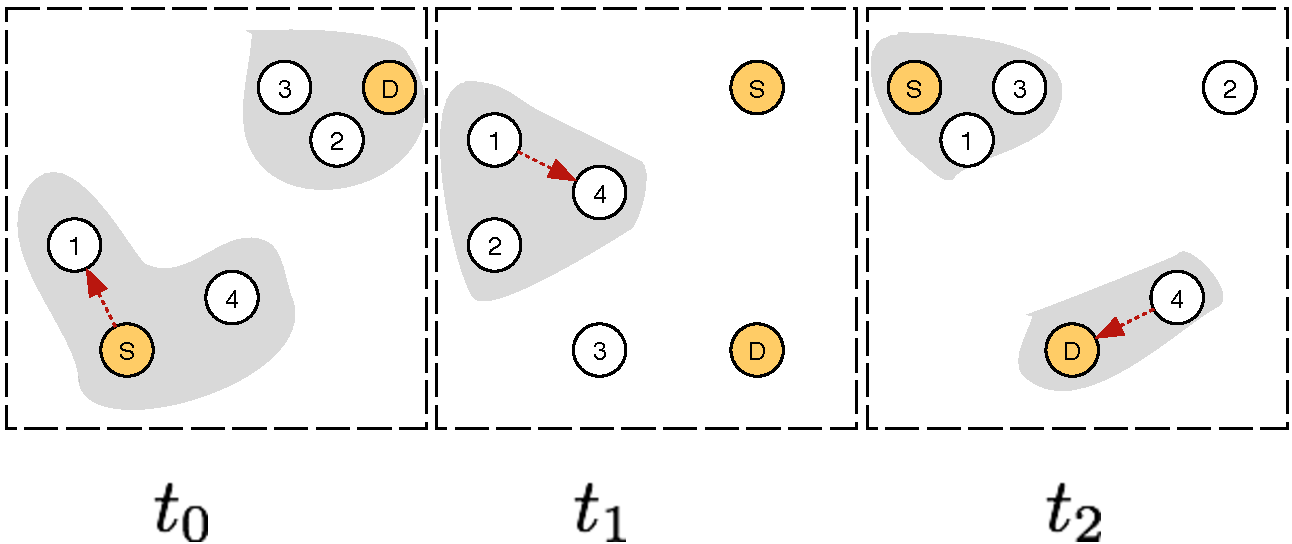
\includegraphics[width=5in]{Figures/SFC.pdf}
	\caption{Store Carry and Forward routing model}
	\label{SFC}
\end{figure}

In OppNet, the messages are delivered using Store-Carry-Forward routing by which  the nodes can exchange data whenever they come in close.
If there is no direct connection from source to destination, data holding nodes will discover their nearest neighbor nodes to forward messages toward the destination node as shown in Fig. \ref{SFC}.
There are several existing works in the literature \cite{Vahdat2000, Harras2005, Neena2013, Lindgren2003,Brendan2005,Boldrini2007,Kerdsri2013} with the aim for 100\% delivery ratio which is quite difficult to achieve especially in sparse network with constraints in energy consumption and message delivery deadline.

Vahdat et al \cite{Vahdat2000} proposed the epidemic routing using  uncontrolled flooding algorithm in which the replication of source data is not restricted with any limits in order to route the message from source to destination in the intermittently connected network.
However, this type of routing incurs significant demand on both bandwidth and buffer.
To address the excess traffic overhead, Khaled et al \cite{Harras2005} proposed a Controlled Flooding  scheme which can limit the flooding by three parameters: Willingness probability, Time-to-Live, and Kill Time.
Nevertheless, flooding based routing performance degrading has been reported in a very sparse network \cite{Neena2013}.

Lindgren et al \cite{Lindgren2003} proposed a prediction based routing called PROPHET (Probabilistic Routing Protocol using History of Encounters and Transitivity) by estimating the delivery predictability to indicate the probability of success in delivering a message to the destination from the local node.
In this prediction based routing category, Brun et al \cite{Brendan2005}  also proposed a protocol utilizing the motion vector of mobile nodes to predict the future location of mobile nodes by using the knowledge of relative velocities of a node and its neighbor nodes to predict the closest distance between two nodes.
Although the prediction based approach can reduce traffic overhead in the network, but it lacks of the aim to improve the performance in extremely low node density and failed in some certain cases which leads to the delivery ratio reduction.

To refine the prediction based routing,  Boldrini et al \cite{Boldrini2007}  proposed the History based routing (HiBOp) which exploits current context information for data forwarding decisions.
Even though, this context based routing approach can reduce the resource consumption in terms of network traffic and storage but it increases the delay which results in significantly less efficient than Epidemic algorithm.
%In our work of content based routing, DORSI protocol \cite{Kerdsri2013} aims to differentiate the messages by their significant in order to improve the delivery ration of important data.
Kerdsri et al \cite{Kerdsri2013} proposed DORSI protocol with the concept of content based routing which aims to classify the data in the network by messages' significance level in order to guarantee the delivery of more important data. 
However, the decreasing in network performance under sparse environment is not mentioned in this proposed protocol.
Overall, the performance of most existing algorithms are degrading in very sparse node density and the energy consumption does not take in to the consideration which is a crucial factor in such mobile sensor devices such as in wildlife monitoring.

%=============================================================================
\section{The proposed Rendezvous based OppNet system}
\label{DRRA:The proposed Rendezvous based OppNet system}
%=============================================================================

\subsection{System model}
\begin{figure*}[!t]
	\centering
	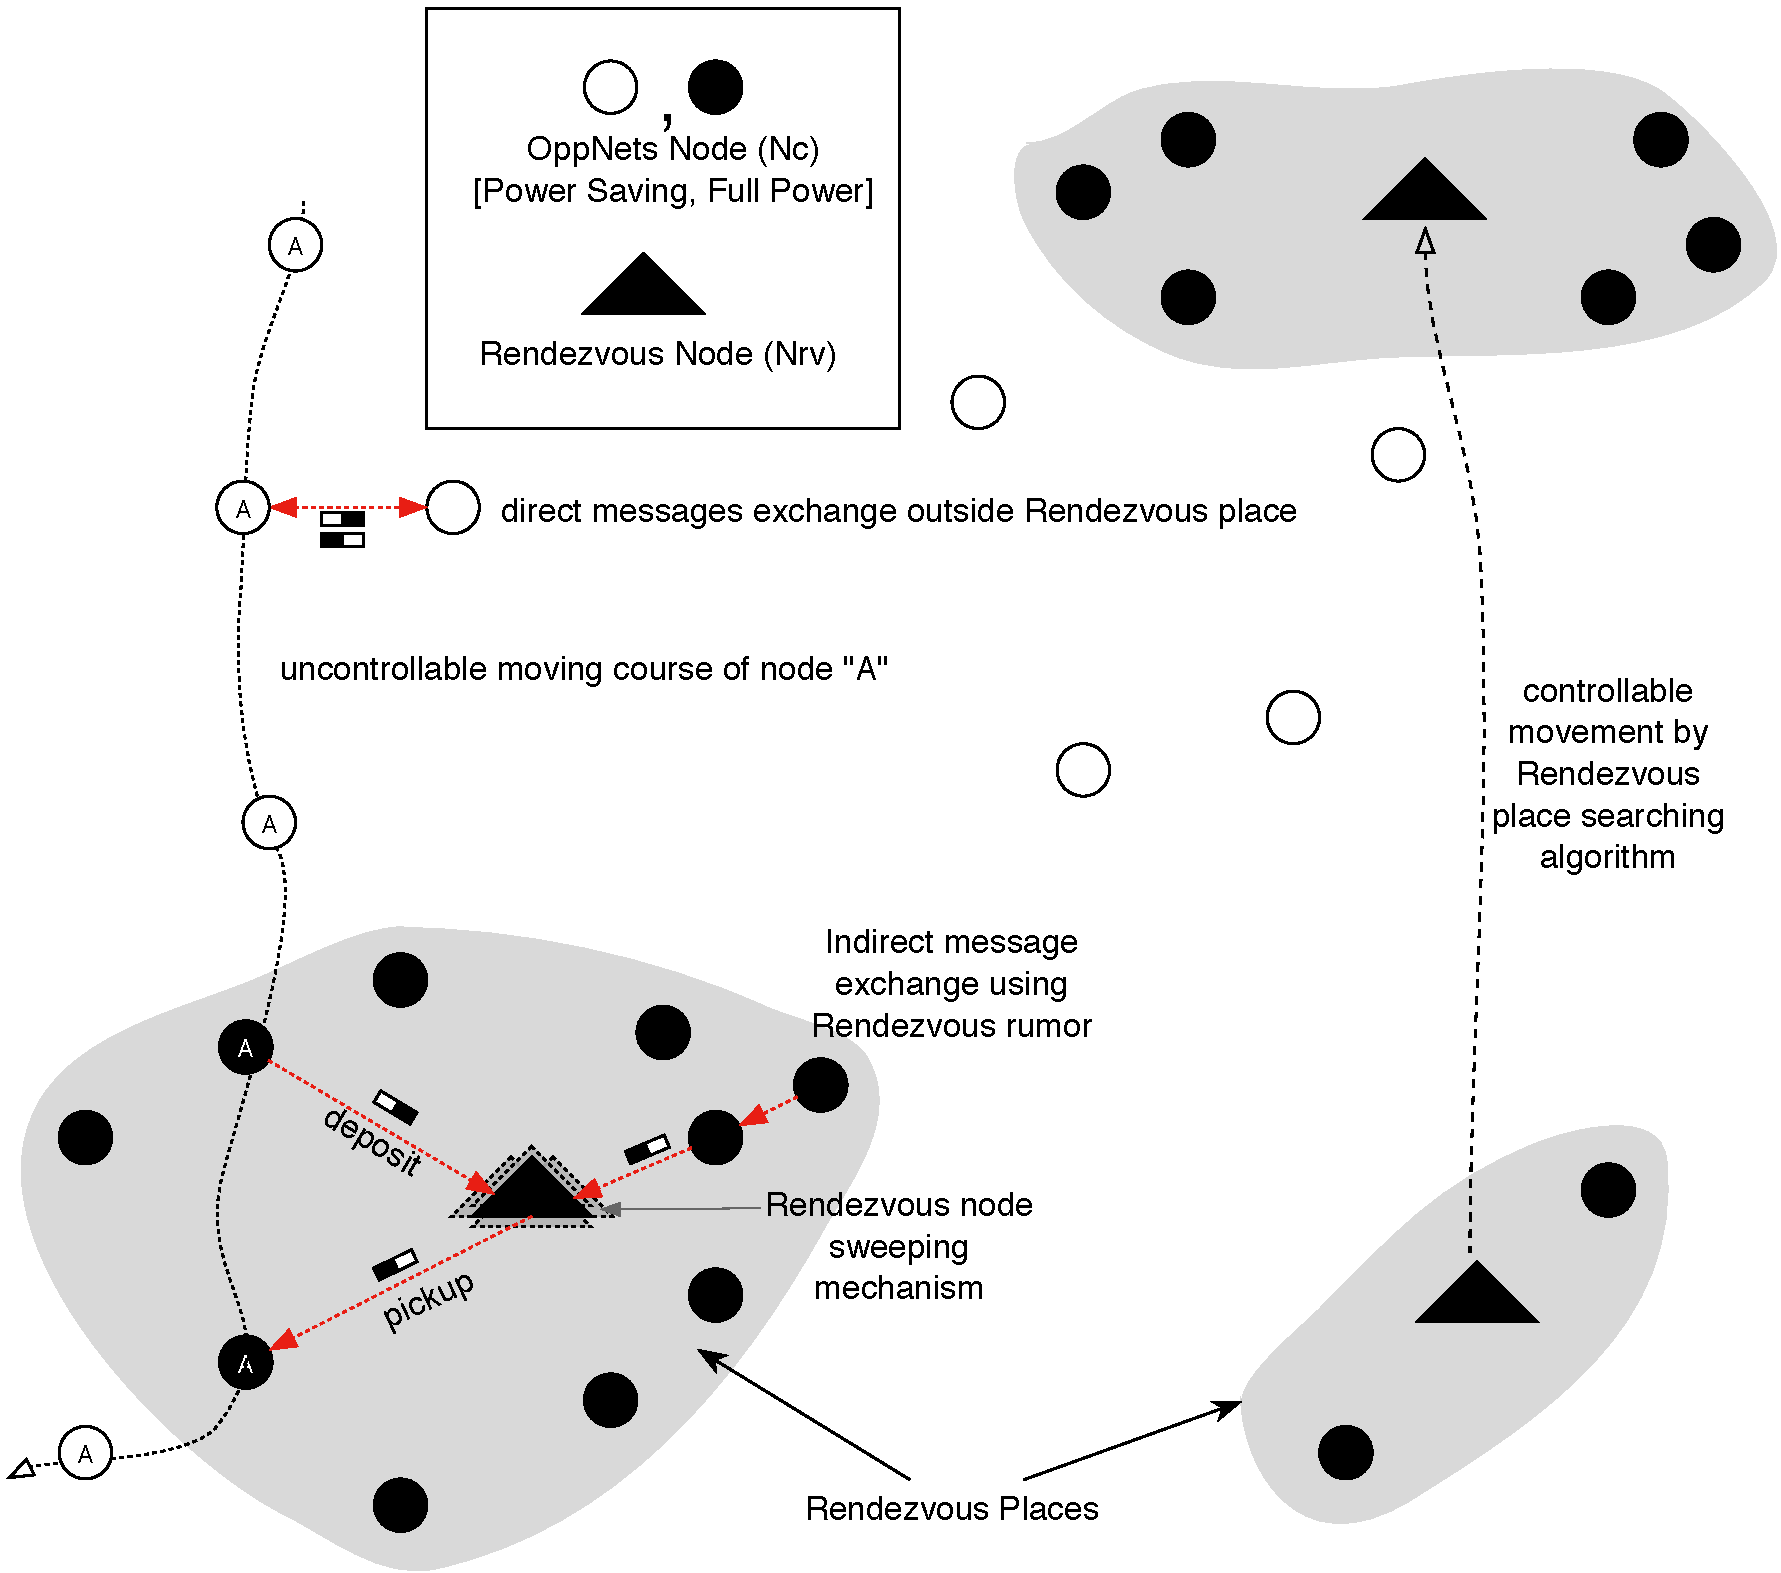
\includegraphics[width=5.5in]{Figures/NewSystemModel.pdf}
	\caption{System model}
	\label{System model}
\end{figure*}

The proposed system is designed to efficiently use the node-gathering area, i.e. Rendezvous place, for depositing the delivered messages as much as possible so that the messages can be picked up by the destination node without requiring the exact timing of direct contact between the node carrying a message and the desired destination node.
In addition, all nodes should reserve its energy as much as possible when they are out of the Rendezvous area.

As shown in Fig. \ref{System model}, the OppNet node, $N_{c}$, whose movement direction is uncontrollable, moves in the system using \textit{Power Saving Mode}  until it reaches the Rendezvous place where it will turn itself to \emph{Full Power Mode} in order to announce its arrival, deposit its carried messages and pick up the messages destined to itself, to/from the Rendezvous place.
The Rendezvous Rumor protocol and Rendezvous Node Sweeping mechanism are used inside the Rendezvous area to let messages being exchanged more effectively without the need of direct contact between the OppNet node and the high-resource direction-controllable Rendezvous node, $N_{rv}$, which is act as the center of the Rendezvous place.
The Rendezvous nodes will move around the OppNet network to create suitable Rendezvous places according to the proposed \emph{Rendezvous Place Searching algorithm}.

\begin{figure}[!t]
	\centering
	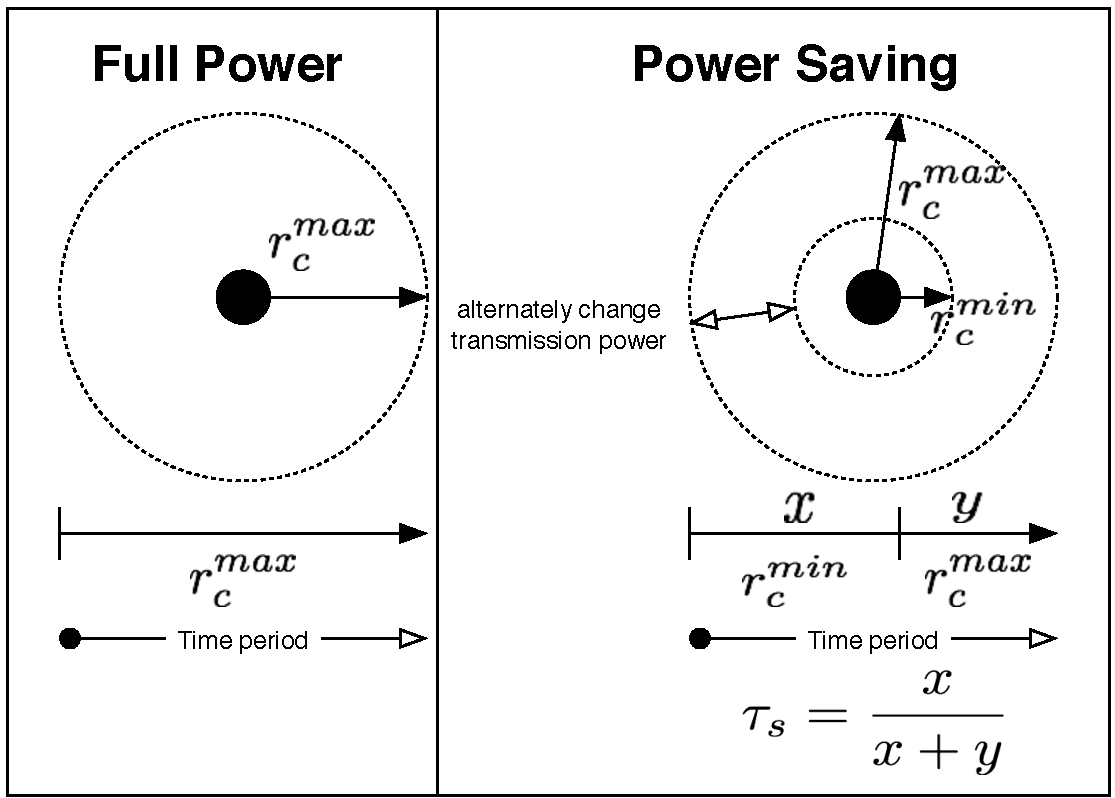
\includegraphics[width=5in]{Figures/OperationalMode.pdf}
	\caption{Operational modes}
	\label{Operational modes}
\end{figure}

\subsection{OppNet node's operational modes: "Full Power" and "Power Saving"}
The OppNet node ($N_{c}$) is a mobile node equipped with the radio interface whose transmission rage is adjustable in range of $[{ r }_{ c }^{ min },{ r }_{ c }^{ max }]$.
The node will operate in either \emph{Full Power mode} or \emph{Power Saving mode} according to its location.
\subsubsection{Full power mode}
In this mode, the node will use its full transmission power, ${ r }_{ c }^{ max }$, to search for nearby nodes and exchange messages.
It will switch to this mode only when getting into the Rendezvous area.

\subsubsection{Power saving mode}
The node, by default, operates in this mode if it is outside the Rendezvous place.
In this mode, it will alternately change its transmission range between ${ r }_{ c }^{ min }$ and ${ r }_{ c }^{ max }$ in the process of searching for nearby nodes.
However, if it receives the searching signal from the other node, it will switch to its full ${ r }_{ c }^{ max }$ immediately in order to increase opportunity to exchange messages with the encountered node as much as possible.
Then, it will switch back to minimum ${ r }_{ c }^{ min }$ when departing from the communicating node.
Besides the ${ r }_{ c }^{ min }$ and ${ r }_{ c }^{ max }$ values, the ratio of the time interval being in it full ${ r }_{ c }^{ max }$ over the whole time period is a configurable parameter,$\tau_{s}$ , as shown in Fig. \ref{Operational modes}.

%=============================================================================
\subsection{Rendezvous place and its Rumor protocol}
\label{DRRA:Rendezvous place and its Rumor protocol}
%=============================================================================

\begin{figure}[!t]
	\centering
	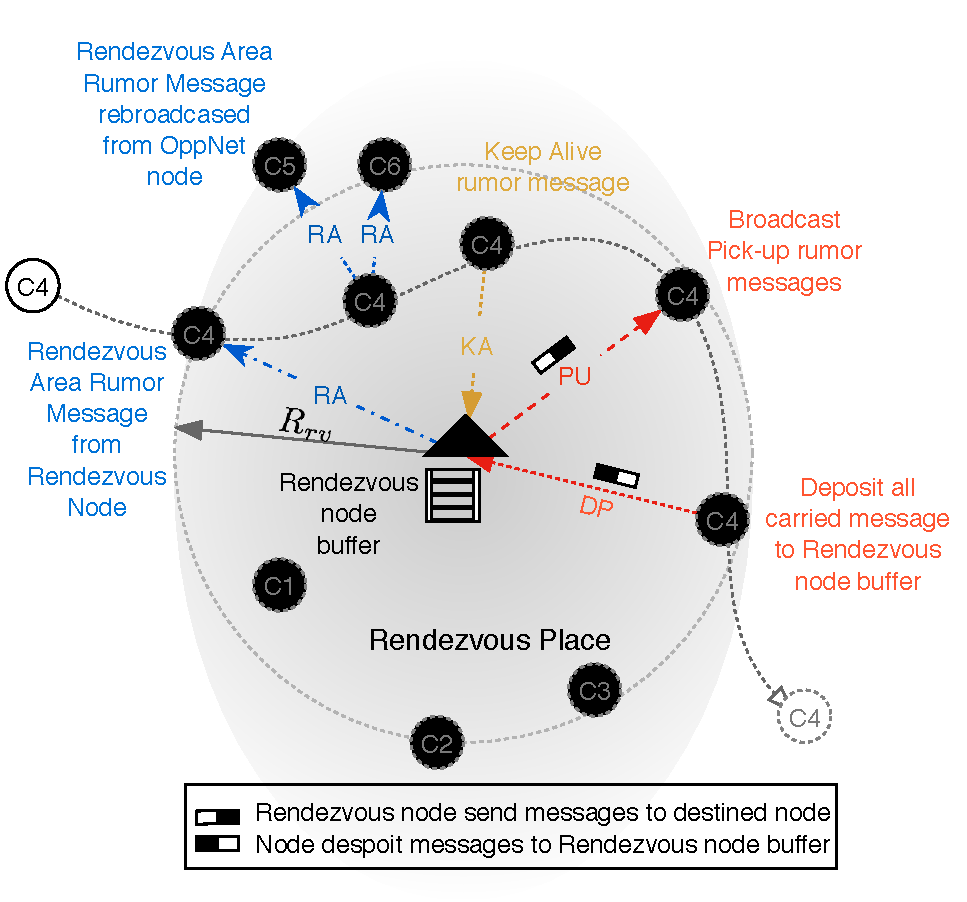
\includegraphics[width=3.5in]{Figures/NewRendezvousPlace.pdf}
	\caption{Rendezvous Place}
	\label{Rendezvous Place}
\end{figure}

The Rendezvous place is a dynamic area centered by a special controllable Rendezvous node, $N_{rv}$.
This $N_{rv}$ node is full of resources such as large message storage and high radio power with maximum transmission range $R_{rv}$.
The Rendezvous place is controlled by the Rendezvous node using Rendezvous rumor protocol.

The area in Rendezvous place is not fixed as the maximum radio range, $R_{rv}$,  of the Rendezvous node, instead it is virtually determined by the covering radio range of the most outer OppNet nodes which can relay the data messages from the Rendezvous node, as shown in Fig. \ref{System model}

When an OppNet node detects the \emph{Rendezvous Area rumor message} $(RA)$ broadcasted from the Rendezvous node, it learns that it enters to the Rendezvous area.
Then, it will switch its operational mode to \emph{Full Power mode} and try to rebroadcast such \emph{Rendezvous Area }rumor message so that the other reachable nearby nodes can learn about Rendezvous place and can adaptively expand the area on-demand.
Additionally, the OppNet node in the Rendezvous area will periodically announce its arrival and upload its carried data messages to the Rendezvous node via the \emph{Keep-Alive} rumor message $(KA)$ and the \emph{Deposit} rumor message $(DP)$ respectively.
Note that all types of rumor messages will be automatically repeated with \emph{duplication filtering} function throughout the area by other OppNet nodes.


\begin{figure}[!t]
\centering
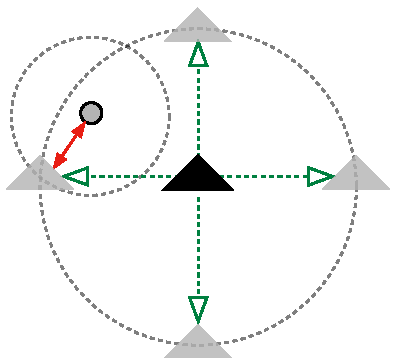
\includegraphics[width=1.5in]{Figures/Sweep.pdf}
\caption{Sweep mechanism}
\label{Sweep mechanism}
\end{figure}

Once the rendezvous node receives the \emph{Keep-alive} rumor message which contains the sending node ID, it will gather all data messages destined to the node ID from its message storage, encapsulate those found messages into the created \emph{Pick-up} rumor message and then broadcast the \emph{Pick-up} message $(PU)$ throughout the Rendezvous area.
On the other hand, the Rendezvous node will keep all of data messages contained in the received \emph{Deposit} rumor messages in its storage for later sending out to the area when the target node appears later as seen in Fig. \ref{Rendezvous Place}. 

In addition to the Rendezvous rumor protocol, the Rendezvous node implements the rumor message sweeping algorithm in order to increase the chance to collect as many rumor messages as possible.
Instead of always being stationary at the center location of the Rendezvous place, the rendezvous node will periodically move to its four directions (North, East, West, South) by the distance of its radio transmission range as shown in Fig. \ref{Sweep mechanism}.
This design lets the OppNet nodes on the edge of Rendezvous node's radio range, whose radio signal may not reach to the Rendezvous node due to the difference in their radio transmission range, can speak back to the Rendezvous node.



\subsection{Rendezvous place searching algorithm}
In the proposed system, the Rendezvous node should move to find the node-gathering area corresponding with the real behavior of OppNet node.


\begin{figure}[!t]
	\centering
	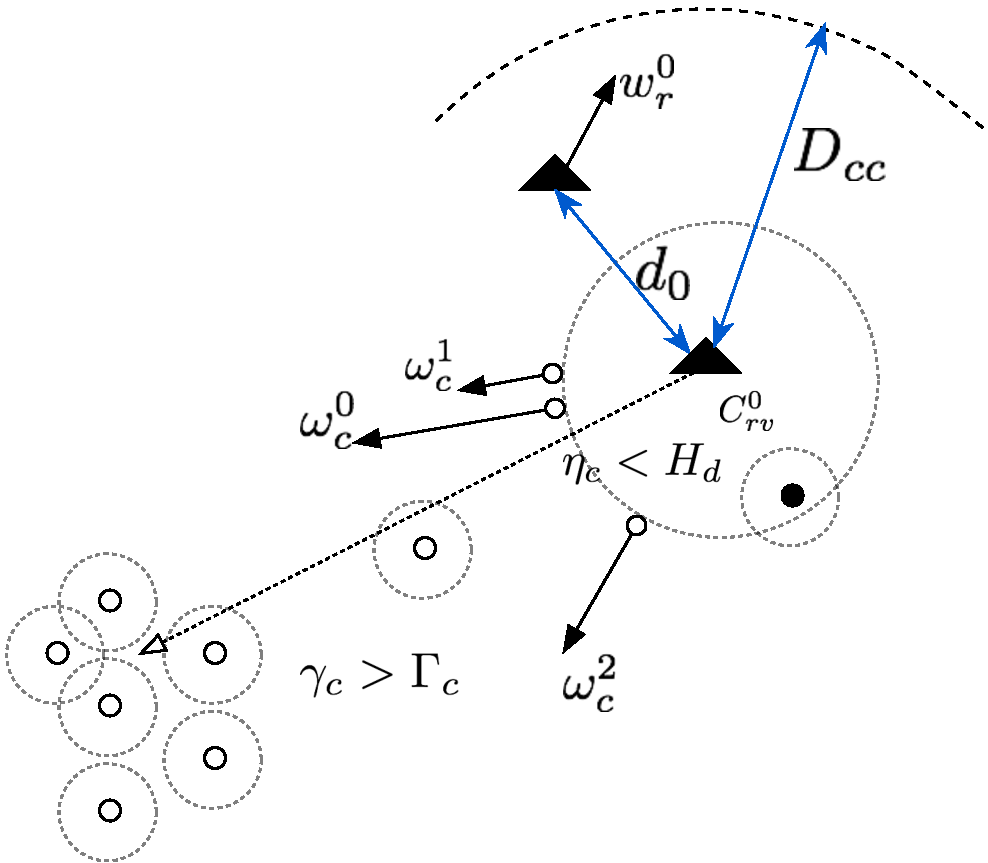
\includegraphics[width=3in]{Figures/Dynamic.pdf}
	\caption{Rendezvous place searching}
	\label{Rendezvous node movements}
\end{figure}


\subsubsection{Predictable behavior OppNet nodes}
In some applications, the movement of OppNet node is somehow predictable.
Take a wildlife monitoring as an example, most animals are usually cyclically gathering in the high supplies area such as along side of the main river of some specific place at some specific time \cite{Yu2007a}.
In these applications, the Rendezvous nodes can be programmed to be located at those areas at the proper time in order to maximize the effectiveness of the proposed system.

\subsubsection{Non-Predictable behavior OppNet nodes}
Without any priori knowledge about OppNet node, the proposed \emph{dynamic Rendezvous Place Searching Algorithm} can be used to guide the Rendezvous nodes to the node-gathering area.
The Rendezvous node will decide to move to the new node gathering location if the number of OppNet node in the current Rendezvous place ($\eta_{c}$) falls below the predefined departure node threshold, $H_{d}$.
The movement direction, $\vec{\Delta}$, will be determined periodically based on the collected statistical data from both previously contacting OppNet nodes and other neighboring Rendezvous nodes as in Eq.\ref{DirectionParameter}.
In the equation, $\vec{w_c}$ is the departure directional unit vector of the contacted OppNet nodes, $\vec{w_r}$ is the directional unit vector of the other Rendezvous nodes and the $\varphi$ is a configurable weighting factor between group of OppNet nodes and group of other Rendezvous nodes in the area.

\begin{eqnarray}
\label{DirectionParameter}
\vec{\Delta} =\sum _{ i=1 }^{ C }{ \vec { { \omega }_{ c }^{ i } }  } + \varphi \sum _{ j=1 }^{ R }{ \delta\left( d_{j} \right)
	\vec { {w }_{ rv }^{ j } }  }
\end{eqnarray}

While the $\delta\left( d_{j} \right)$ is the on-off function to include only the other Rendezvous nodes whose distance $d_j$ is the range of cut-off distance perimeter, $D_{cc}$, and the  $C$ and $R$ are the number of contacted OppNet nodes and the number of other Rendezvous nodes respectively.

\[\delta \left( { d }_{ j } \right) =\begin{cases} 1\quad ;\quad { d }_{ j }\quad \le { \quad D }_{ cc } \\ 0\quad ;\quad { d }_{ j }\quad >{ \quad D }_{ cc } \end{cases}  \] 

The Rendezvous node will decide to stop at the expected node-gathering area when the number of OppNet nodes in the current Rendezvous place ($\gamma_{c}$) become greater than the predefined Rendezvous place node threshold, $\Gamma_{c}$ as shown in Fig. \ref{Rendezvous node movements}. 

%=============================================================================
\section{Evaluation}
\label{DRRA:Evaluation}
%=============================================================================
The objective of the evaluations is to analyze the performance of our proposed protocol on the sparse network environment comparing with traditional OppNet protocols.
We compare both predictable and non-predictable behavior OppNet nodes with the commonly well-known Epidemic protocol\cite{Vahdat2000} under different node density environments.


\subsection{Simulation setup}
We setup a simulation environment using ONE (Opportunistic Network Environment) \cite{Keranen2009b}, which is a powerful tool designed for running opportunistic network simulation with various routing protocols and different movement models.
All the results are obtained by averaging over a few hundreds independent simulation runs with different seeds.
For the OppNet simulation model, the main parameter that largely effected the evaluation performance is the movement model.
In our evaluation, we deploy Group movement model instead of the most commonly used, Random Way Point (RWP) model \cite{Batabyal2012}, to correctly capture the the actual behavior of node movements.
In fact, several multi-hop wireless network scenarios are most realistically represented using Group movement model \cite{Blakely2004} which represents the random motion of a group of mobile nodes as well as the random motion of each individual mobile node within the group.
This is the vital case for modeling the routing simulation in OppNet since the movements in several cases are in swarm behavior, in which nodes are aggregates together and moving in some directions, such as the movement of animals or military tactical operations.
The other parameters that mainly effect the evaluation performance are the area of operation, the wireless range of the nodes, node velocity and spatial location of the nodes \cite{Batabyal2012}. 
In our simulation, we fix the number of nodes while increasing and decreasing the area of operation which results in wide range of node density parameter for evaluation.
Node density ($\lambda$) is defined as the number of nodes per unit area. 
If $N$ nodes are distributed in a square grid of size $M \times M \quad{ m }^{ 2 }$ then the $\lambda$ is given by $\lambda =\frac { N }{ { M }^{ 2 } } $ . 
The wireless range of our OppNet node can be adjusted depending on the environment while the node velocity is equal to the normal human walking speed.
The common parameters are summarized in Table \ref{table_parameters}.
%%%%%%%%%%%%%%%%%%%%%%%%%%%%%%%%%%%%%%%%%%%%%%%%%%%%%%%%%%%%%%%%%%%%%
\subsection{Metric}
%%%%%%%%%%%%%%%%%%%%%%%%%%%%%%%%%%%%%%%%%%%%%%%%%%%%%%%%%%%%%%%%%%%%%

\begin{table}[!t]
	\renewcommand{\arraystretch}{1.3}
	\caption{simulation variables}
	\label{table_parameters}
	\centering
	\begin{tabular}{|c|c|c|}
		\hline
		Parameters         &  $N_{c}$ & $N_{rv}$ \\ \hline
	%	Simulation Time     & \multicolumn{2}{|c|}{10800 Seconds }  \\ \hline
		Message Size       &  \multicolumn{2}{|c|}{500 KB - 1 MB}        \\ \hline
		% Node Buffer         & \multicolumn{2}{|c|}{500 MB}&  10 GB      \\ \hline
		Maximum Radio Range & 30 Meters  & 100 Meters \\ \hline
		Transmission Speed &  \multicolumn{2}{|c|}{ 54 Mbps   }        \\ \hline
		Router             & \multicolumn{2}{|c|}{ DRRA | Epidemic   } \\ \hline
		Moving Speed       &   \multicolumn{2}{|c|}{0.5 - 1.5 m/s }        \\ \hline
		Movement Model     &   \multicolumn{2}{|c|}{Group Movement Model  }      \\ \hline
	\end{tabular}
\end{table}

Opportunistic routing protocols are commonly evaluated by delivery ratio, median latency and network overhead.
%%
In this paper, we focus on delivery ratio and network overhead in term of energy consumed to deliver a message within a specific message deadline.
%%
We assume that all messages delivered within the deadline has no difference in protocol performance.

% Opportunistic routing protocols are commonly evaluated by delivery ratio, median latency and network overhead.
% However, we required specific composite metrics in order to clearly observe the performance of our proposed protocol.
% In our evaluation we consider the following metrics:

\paragraph{Delivery ratio ($D_{r}$)} is defined as the ratio of the total number of messages successfully delivered within the deadline ($ { M }_{ delivered }$) to the total number of messages created from the source nodes that need to be delivered ($ { M }_{ created }$) as shown in Eq. \ref{delivery_ratio}.

	\begin{equation}
	\label{delivery_ratio}
	D_{r} =\frac { { M }_{ delivered } }{ { M }_{ created } } 
	\end{equation}

\paragraph{Energy consumption ($E_{c}$)} is defined as the amount of energy consumption required by all related OppNet nodes to deliver one $M_{created}$ message.
%all $M_{created}$ messages.
%%
% We simplify the energy consumption model by only considering for the communication energy consumption of the wireless interface to transmit all necessary protocol packets, $M_{packet}$.
We simplify the energy consumption model by only considering for the communication energy consumption of the wireless interface to transmit a message by determining the number of all necessary protocol packets, $M_{packet}$ per number of $M_{created}$ messages.
%%
To transmit an $L$ bit-length packet using radio interface with transmission length, $d$, the consumed energy, ${ E }_{ T }$, can be determined by Eq.\ref{eq:enegy} \cite{Yang2010, Wang2006}, where $\alpha$ is the power loss component with $\alpha \in \left[ 2,4 \right]$ and $\epsilon { f }_{ s }\left[ J/(bit/{ m }^{ \alpha  }) \right]$ is the amount of energy consumed by an amplifier to transmit one bit data at an acceptable quality level.

\begin{eqnarray}
	\label{eq:enegy}
	{ E }_{ T }\quad =\quad L\cdot  { \epsilon  }_{ fs } \cdot  { d }^{ \alpha  }
\end{eqnarray} 

As a result, the energy consumption ($E_c$) can be derived as Eq. \ref{eq:enegy_consumed} 

\begin{eqnarray}
	\label{eq:enegy_consumed}
	{ E }_{ c }\quad =\quad \frac{M_{packet}}{M_{created}} \cdot L_p \cdot  { \epsilon  }_{ fs } \cdot  { r }^{ 2 }
\end{eqnarray} 

Note that $L_p$ is the size of protocol packet, $r$ is the radio transmission range of the protocol packet and $\alpha$ is equal to two in our simulations.
%%
\paragraph{Protocol performance ($P_{\Psi}$)} is a composite metric to capture the gain in both delivery capability and energy saving capability of a specific protocol, compared with the baseline protocol, Epidemic.
%%
The $P_{\Psi}$ can be calculated from Eq. \ref{eq:protocol_performance}.

\begin{eqnarray}
\label{eq:protocol_performance}
{ P }_{ \Psi }= {{ D }_{ r }^{ P,B }} \cdot \frac { 1 }{ { E }_{c}^{ P,B } } 
= \frac {{ D }_{ r }^{ P }}{{ D }_{ r }^{ B } } \cdot \frac{{ E }_{c}^{ B }}{{ E }_{c}^{ P }}
\end{eqnarray}

In this Equation, $P$ is the target protocol while $B$ is the baseline protocol (Epidemic protocol, for example) to be used as comparative energy reference.

%%%%%%%%%%%%%%%%%%%%%%%%%%%%%%%%%%%%%%%%%%%%%%%%%%%%%%%%%%%%%%%%%%%%%
\subsection{Simulation Results}
%%%%%%%%%%%%%%%%%%%%%%%%%%%%%%%%%%%%%%%%%%%%%%%%%%%%%%%%%%%%%%%%%%%%%
This section shows the results of the different sets of simulation runs that have been performed to study the performance of the proposed routing protocol and its behavior when changing the protocol's key parameters.
%%
\subsubsection{General protocol performance}

\begin{figure}[!t]
	\centering
	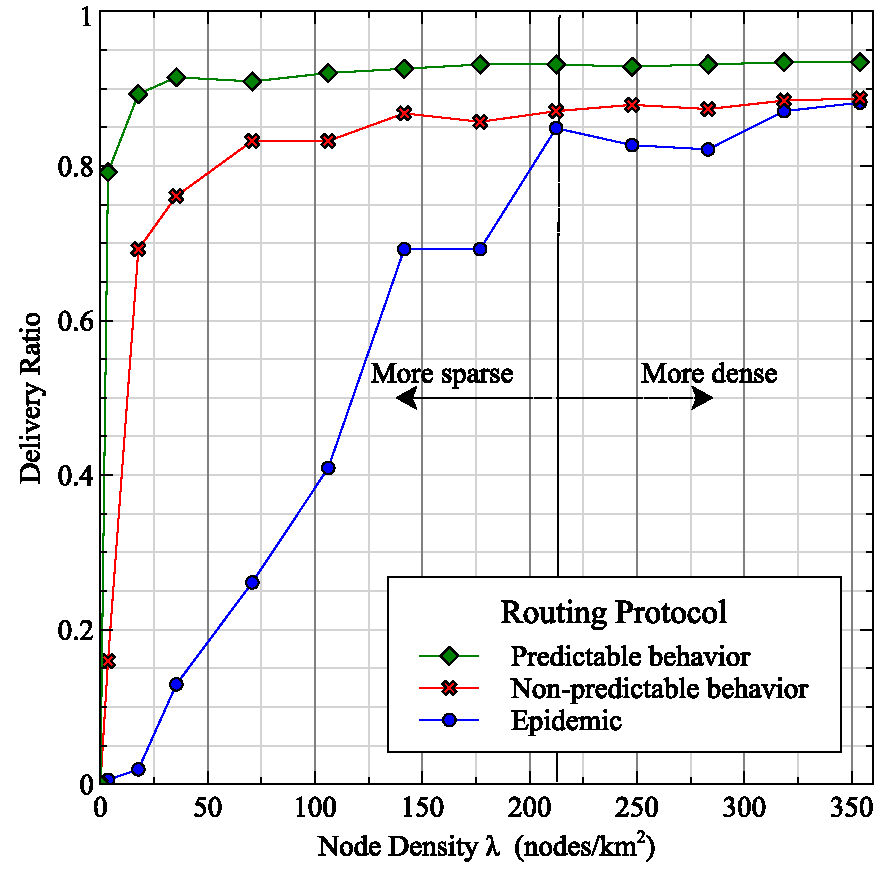
\includegraphics[width=2.5in]{Graphs/DeliveryRatio.pdf}
	\caption{Delivery Ratio per Node Density}
	\label{Delivery Ratio per Node Density}
\end{figure}

\begin{figure}[!t]
	\centering
	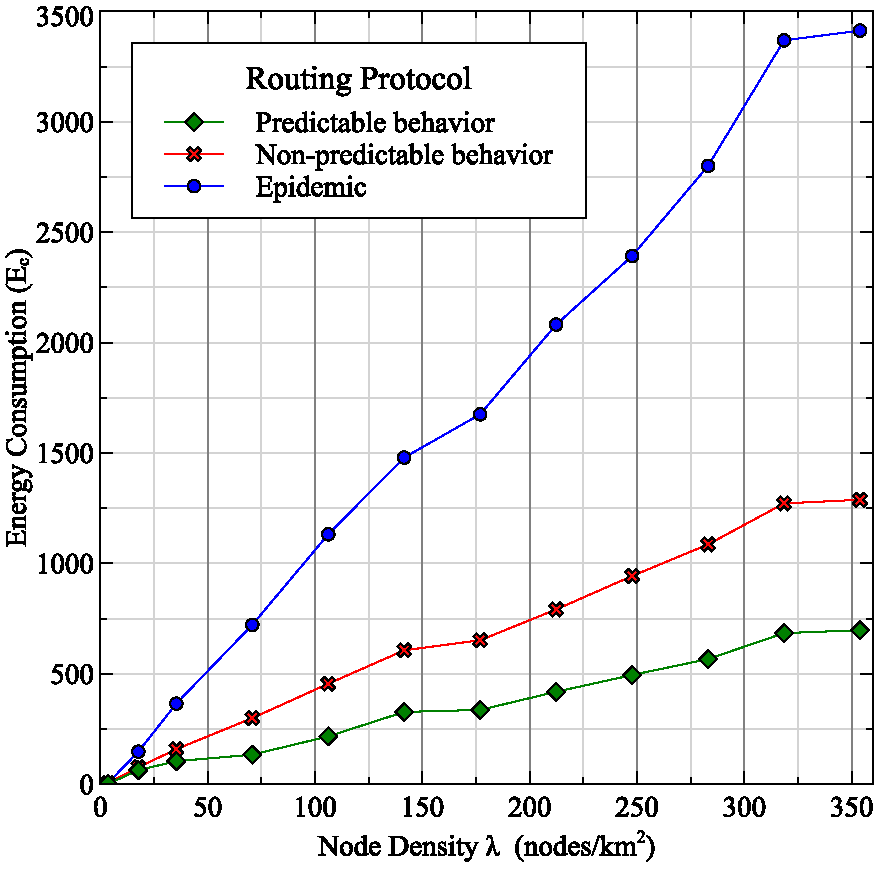
\includegraphics[width=2.5in]{Graphs/EnergyConsumption.pdf}
	\caption{Energy Consumption per Node Density}
	\label{Energy Consumption per Node Density}
\end{figure}

\begin{figure}[!t]
	\centering
	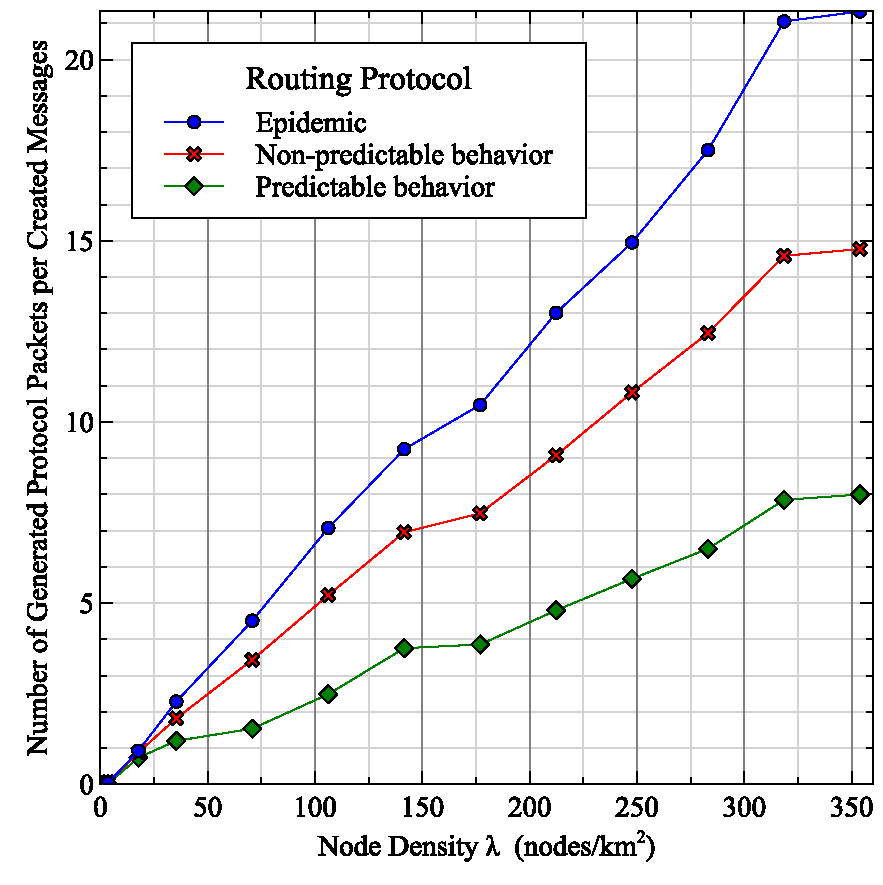
\includegraphics[width=2.5in]{Graphs/messages.pdf}
	\caption{Number of Generated Protocol Packets per Created Messages on Node Density}
	\label{Number of Generated Protocol Packets}
\end{figure}

\begin{figure}[!t]
\centering
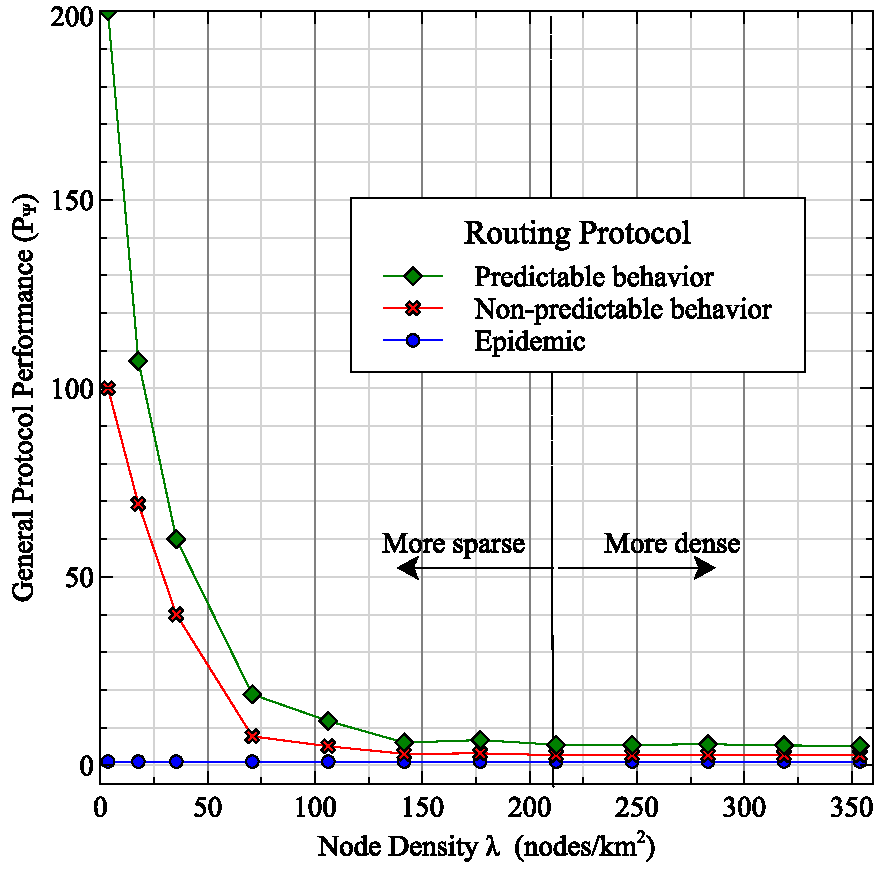
\includegraphics[width=2.5in]{Graphs/ProtocolPerformance.pdf}
\caption{General Protocol Performance per Node Density}
\label{General Protocol Performance per Node Density}
\end{figure}

Firstly, the comparison of delivery ratio is shown in Fig. \ref{Delivery Ratio per Node Density}, where $x-axis$ represents the node density (the number of nodes in the area of one $km^2$) and $y-axis$ shows the delivery ratio.
In our simulation, we assume the environment of one Rendezvous node and the ratio of time interval between full power and power saving, $\tau_s$ of 0.5.
%
Fig. \ref{Delivery Ratio per Node Density} shows that our proposed protocols gain slightly better delivery ratio in the dense environment.
On the other hand, the proposed protocols gain significantly higher delivery ratio in the sparse environment by maintaining the ratio up to 80\%, even when node density is as low as 50 $nodes/km^2$ in non-predictable behavior or as low as 5 $nodes/km^2$ nodes in predictable behavior.
Over all in average, our proposed protocols gain approximately 40\% higher delivery ratio than existing traditional Epidemic routing in sparse networks.

The reason behind the behaviors from this result is that the proposed Rendezvous concept can facilitate message exchanging process between nodes passing through the same area but on the different time-line as designed.
%%
Those nodes coincidence on both time and space domain are likely to happen more in dense network but will become rarely to happen when the network is more sparse.
%% 
In addition, with the knowledge of node gathering area (predictable behavior), the delivery ratio of the proposed protocol can be further increased especially in the extremely low node density. 

Secondly, the energy consumption ($E_c$), which is another vital factor in opportunistic network where most mobile nodes are usually equipped with limited power resources, is shown in Fig. \ref{Energy Consumption per Node Density}.
%%
The $x-axis$ represents node density and $y-axis$ is the $E_c$ in unit of energy consumption per 1,000 messages.
%%
This graph shows that the value of $E_c$ linearly increases when network become more dense.
%%
The trend on the graph is similar to the number of generated protocol packets per created messages on node density graph in Fig. \ref{Number of Generated Protocol Packets}.
%%
The predictable behavior save 80\% less energy consumption than Epidemic protocol while non-predictable behavior can save around 60\% of Epidemic counterpart.
%%
On the other hand, the number of generated protocol packets per created messages of predictable behavior is 60\% and for non-predictable behavior is 30\% lower than Epidemic protocol.
%%The reason for this behavior
The reason of $E_c$ rising in the dense environment results from the increasing of node meeting activities from growing number of nodes which generating more number of messages.
%
The trend similarity from Fig. \ref{Energy Consumption per Node Density} and \ref{Number of Generated Protocol Packets} is derived from the increasing number of messages in Eq. \ref{eq:enegy_consumed} which resulting in the rising in energy consumption. 
%%
Our proposed protocols require less number of generated messages while presenting significant lower $E_c$ which is the result from the fact that the Rendezvous protocols utilize less average wireless radius.

Combining both gains in delivery ratio and energy consumption saving, the proposed general protocol performance can be seen in Fig. \ref{General Protocol Performance per Node Density}. 
%
The Epidemic is used as the based-line protocol in $P_{\psi}$ calculation so its value in Fig. \ref{General Protocol Performance per Node Density} is 1.
%
The proposed protocol performance can achieve up to 20 times of the existing Epidemic when network is very sparse and on average about 5-10 times in general network environment.
al Epidemic protocol.

%%%%%%%%%%%%%%%%%%%%%%%%%%%%%%%%%%%%%%%%%%%%%%%%%%%%%%%%%%%%%%%%%%%%%%%%%%
\begin{figure}[!t]
\centering
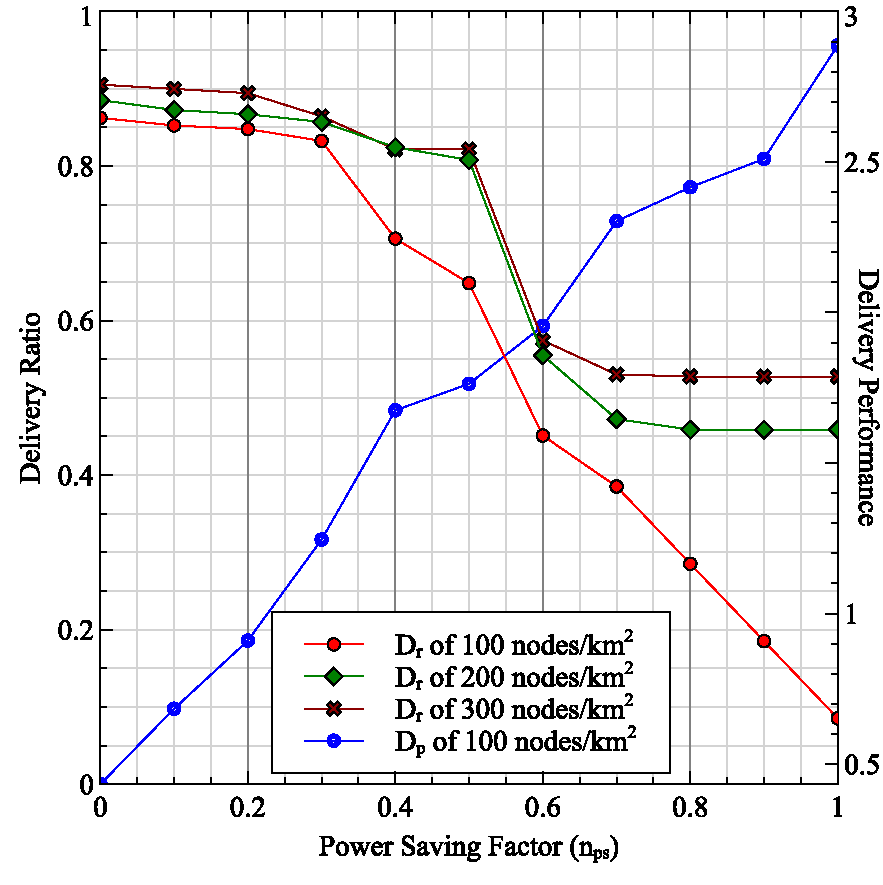
\includegraphics[width=2.5in]{Graphs/NpsDeliveryPerformanceAndDeliveryRatio.pdf}
\caption{Delivery Ratio and Energy Consumption on Power Saving Factor}
\label{The Optimum between Delivery Ratio and protocol Performance}
\end{figure}

\subsubsection{Impact from power saving factor}

In this subsection, we study protocol parameters relevant to the power saving factor and the trade-off between power consumption and delivery ratio.
%
We define the power saving factor, $n_{ps}$ as the composite parameters of the proposed protocol as in Eq. \ref{nps}.
%
\begin{equation}
{ n }_{ ps }={ \tau  }_{ s }\cdot \frac { { r }_{ c }^{ max }-{ r }_{ c }^{ min } }{ { r }_{ c }^{ max } } 
\label{nps}
\end{equation}
The $n_{ps}$ is mainly calculated from the time being in power saving mode, $\tau_s$ and the portion of energy consumption used when being in such power saving mode.
%
The value of $n_{ps}$ is in [0,1] range where its minimum value (no saving) represents either OppNet nodes never operate in power saving mode of the proposed protocol or the maximum energy consumption ($r_c^{min} = r_c^{max}$) is used in such mode.
%
The opposite behavior in power saving mode is for the maximum $n_ps$.
%
Fig. \ref{The Optimum between Delivery Ratio and protocol Performance} shows both delivery ratio ($D_r$ on solid line) and energy consumption ($E_c$ on dash line) when varying power saving factor ($n_{ps}$) for the node density ($\alpha$) = 100 and 300 $nodes/km^2$.
%
The graph shows that when $n_{ps}$ increases the value of $E_c$ and $D_r$ decreased as expected.
%
The delivery ratio for more sparse network significantly drops when the $n_{ps}$ increases because the saving factor can degrade the delivery performance if the nodes spend more time in saving mode.
%
In fact, the optimum of $n_{ps}$ depends on the real applications.
%
In the application with the level of acceptable minimum $D_r$ as a threshold, we can select the $n_{ps}$ that gives the minimum $E_c$.
%
On the other hand, we can select the $n_{ps}$ that gives the maximum $D_r$ if the threshold of acceptable maximum $E_c$ is defined.
%
Finally, if both the minimum $D_r$ and maximum $E_c$ are defined, we can get the $n_{ps}$ value that suit the application.

%%%%%%%%%%%%%%%%%%%%%%%%%%%%%%%%%%%%%%%%%%%%%%%%%%%%%%%%%%%%%%%%%%%%%%%%%%

\subsubsection{Other network environment parameters}

\begin{figure}[!t]
	\centering
	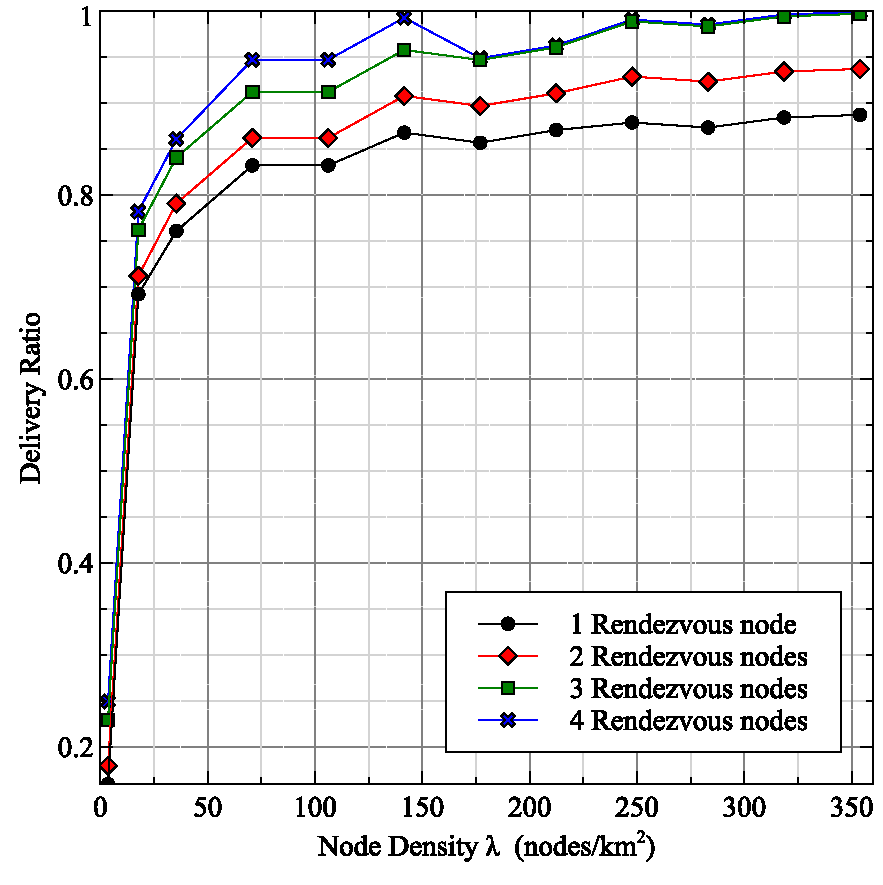
\includegraphics[width=2.5in]{Graphs/MultipleRVs.pdf}
	\caption{Multiple Rendezvous Nodes}
	\label{Multiple Rendezvous Nodes}
\end{figure}

\begin{figure}[!t]
\centering
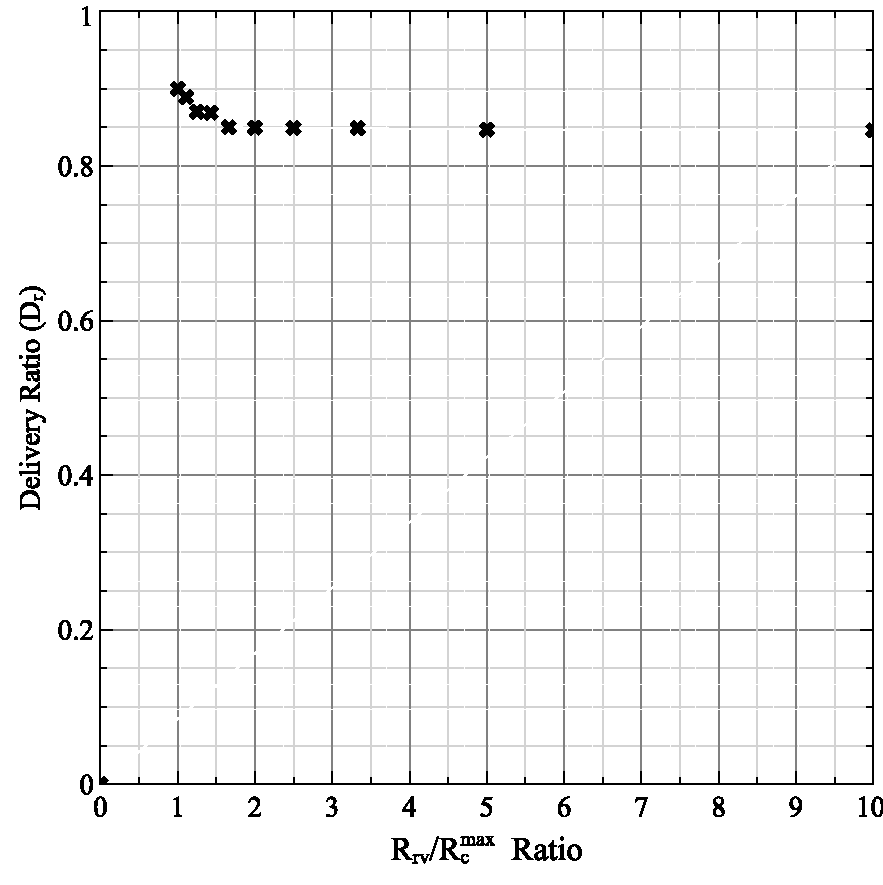
\includegraphics[width=2.5in]{Graphs/RcmaxRrv.pdf}
\caption{$R_{rv}$/$R_c^{max}$ ratio}
\label{RrvRcmaxRatio}
\end{figure}

\begin{figure}[!t]
\centering
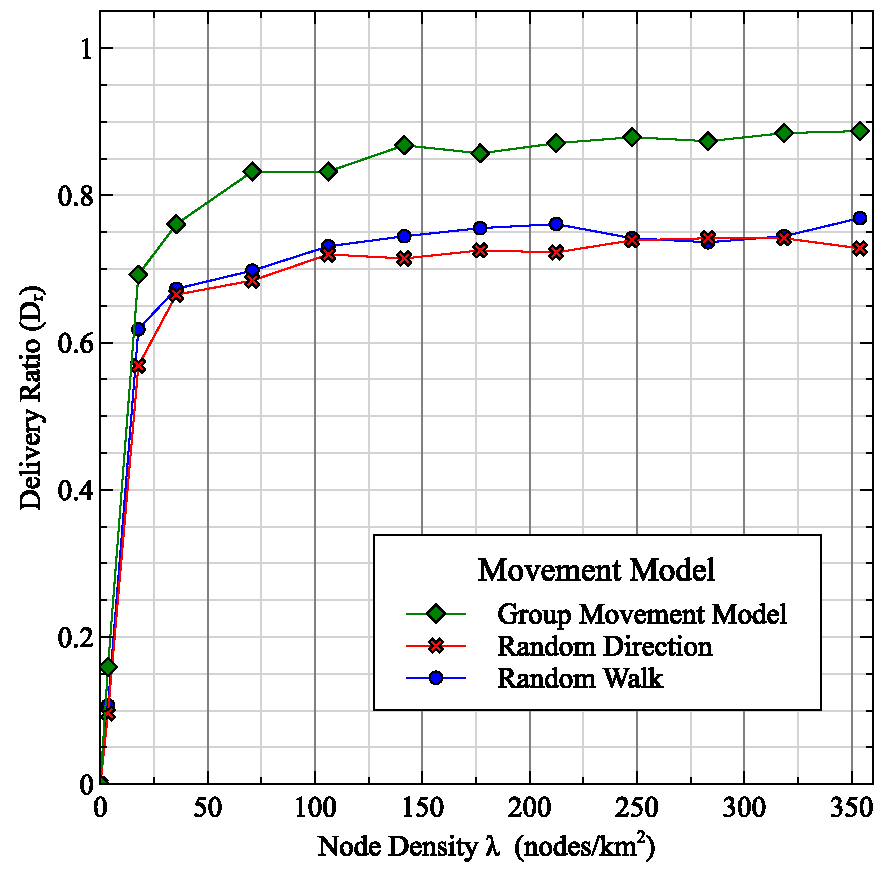
\includegraphics[width=2.5in]{Graphs/movement.pdf}
\caption{Movement Model Comparison}
\label{Movement Model Comparison}
\end{figure}

In this subsection, we investigate other protocol and environmental parameter which may have effect to the proposed protocol performance.
%
Fig. \ref{Multiple Rendezvous Nodes} presents the variation on the number of Rendezvous nodes to analyze the impact on delivery ratio per node density.
%
This graph shows that more Rendezvous nodes can achieve more $D_r$ as expected.
%
In Fig. \ref{RrvRcmaxRatio}, the effect of $R_{rv}/R_c^{max}$ ratio on delivery ratio is studied.
% 
By increasing $R_{rv}$ (maximum radio transmission of Rendezvous node), the $D_r$ will not increase but slightly decrease.
%
This is the result from the asymmetric in transmission range of OppNet nodes which can degrade the delivery ratio performance in Rendezvous area, since the nodes with longer transmission range can send the messages to other nodes with shorter range, but can not receive the messages back.
%%
Finally, Fig. \ref{Movement Model Comparison} shows that our proposed Rendezvous protocol performance will drop if node movement become more random since the proposed protocol utilizes the group gathering behavior to increase message exchanging activities.

%=============================================================================
\section{Conclusion}
\label{DRRA:Conclusion}
%============================================================================= 

Opportunistic Routing techniques can be applied in  plentiful variety of scenarios such as military network or wildlife monitoring. 
%
In this paper, we investigate the use of Rendezvous points in opportunistic network routing to increase the delivery ratio in extreme sparse network environment.
%
This novel protocol proposes the two new types of node, Rendezvous node and OppNet node, which can help maintaining the messages in one place as long as possible in order to bridge the gap of time and space domain.
%
In this Rendezvous place, the passing nodes can announce, deposit and pickup their own messages without meeting with other nodes that carried desired messages.
%
The size and shape of  Rendezvous place can be adapted to the environment of OppNet nodes in the area.
%
We define our routing model in two functions: predictable  and non-predictable behavior OppNet node functions.
%
The result suggest that our protocols perform significant higher in general protocol performance which is the trade off of delivery ratio per energy consumption.
%
We can simply imply that if the location of rendezvous place can be predicted, we can achieve highest overall performance.
%%
In the future work, this concept of smart node can be further extend to increase the intelligence of the node since the technologies can be rapidly advanced.



%!TEX root = thesis.tex
\chapter{Data-wise Opportunistic Routing with Spatial Information}
\label{DORSI}
% \SVN $Revision: 838 $
% \SVN $Author: sgordon $
% \SVN $Date: 2014-05-12 13:30:42 +0700 (Mon, 12 May 2014) $
% \SVN $URL: https://sandilands.info/svn/Common/Styles/siitthesis/chapter4.tex $
As for now, the routing algorithms for opportunistic network has been barely concerned about the content of data. 
%%
The routing decision for this type of network is usually based on node topology environment. 
%%
However, there are several data dissemination methods based on the context of data. 
%%
Yazhou et al. \cite{Jiao2009} proposed the data dissemination in DTN based on content classification which classifies the forwarding messages by their content, every node only requests the message that it is interested in. 
%%
This research showed that this method can provide low overhead while maintaining high delivery rate and low delivery latencies compared to epidemic routing. 
%%
While in other content-based network scheme \cite{Carzaniga2004}, message content is structured as a set of attribute/value pairs, and a selection predicate is a logical disjunction of conjunctions of elementary constraints over the values of individual attributes. 
%%
Both techniques differ from DORSI in the sense that they route all messages by sets of rules while our protocol route messages differently depend on their priority class.

A number of related researches attempt to address the main criticism of flooding based routing protocol in term of network congestion. 
%%
APRA \cite{Jin2009} arranges the forwarding sequence and the dropping sequence based on their assigned priority. 
%%
This priority is determined by the TTL, Delivery Predictability, and Replication Density. 
%%
While Joe et al. \cite{Joe2010} developed a DTN message priority routing protocol by modify the spray and wait \cite{Spyropoulos2005} flooding-based routing protocol. 
%%
However, these prioritizing mechanisms aim to rank the messages by defined matrices which involving network topology. 
%%
In contrast, DORSI protocol routes the data based solely on the content of data itself.

Although all of the above mentioned the routing method by the content of message to limit the number of message flooding in the network. The messages traversing in the network are treated the same except containing different attributes. The routing decision depends on the sets of rules and nodes. In this chapter, we propose a new routing technique to assure the deliverable of important data while maintain the lower message replicas. The routing decision depends on the class of data itself. In addition, we improve the overall performance by appending the geographic information for forwarding node selection.

In this chapter, we present a routing protocol in opportunistic environment that dynamically prioritizes the candidate messages based on the content of the data. Since security is an increasing concern in military and other critical operation mission, it is vital to route data of different sensitivities differently. The most significant and sensitive data should be guaranteed its higher level of delivery and protection than common data. However, only few works have applied the well-defined information sensitivity concept such as Multi Level of Security (MLS) \cite{Kotrappa2010,marking2010} to network information such as routing information, QoS signaling and other management information \cite{Winjum2008}.

In this routing scheme, we purpose to incorporate the information sensitivity concept into the messages in order to route the data differently in compliance with the classes of messages. To the best of our knowledge, this method has not been fully explored in the existing literatures. In this research, we extend our previous work \cite{Kerdsri2012} by generalizing information sensitivity parameters and involving spatial information into routing decision to improve the network efficiency. We conducted Opportunistic Network Environment (ONE) simulation \cite{Keranen2009b} to evaluate the performance of DORSI protocol.
%=============================================================================
\section{Opportunistic network model}
\label{DORSI:Opportunistic network model}
%=============================================================================

\begin{figure}[!t]
\centering
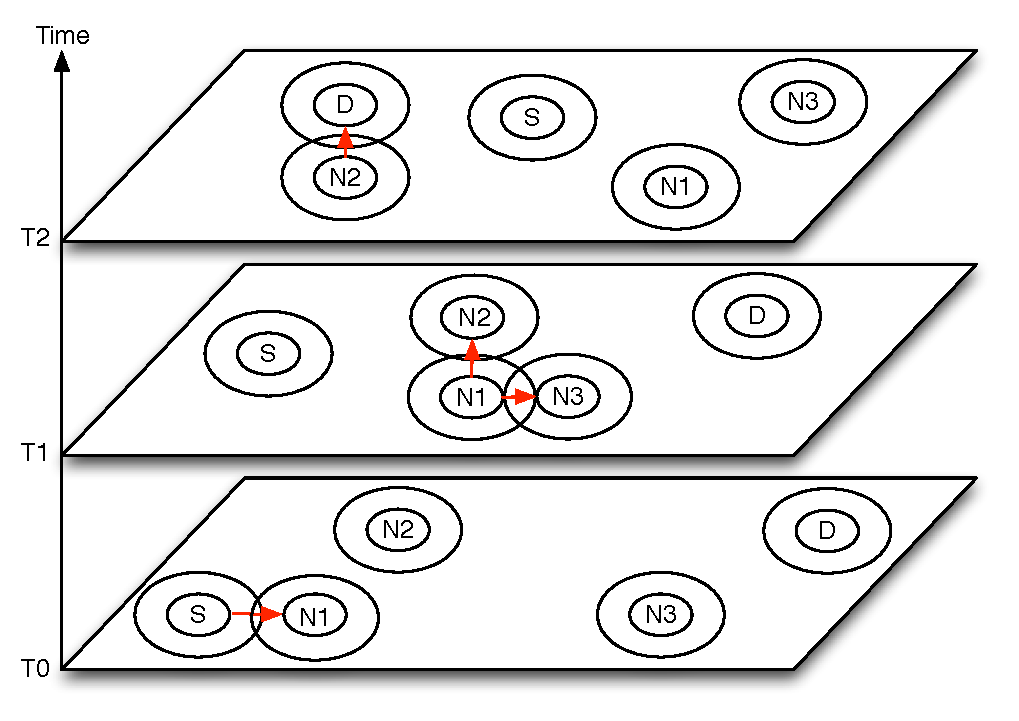
\includegraphics[width=5in]{Figures/OpportunisticNetworkNodel.pdf}
\caption{Opportunistic network model}
\label{Opportunistic network model}
\end{figure}

Since opportunistic network commonly operates in multi-hop wireless ad-hoc network environment, links may be disrupted or shut down periodically when nodes move away or absent which resulting in intermittent connectivity \cite{Moreira2011}. As a result, nodes require to communicate with each other via opportunistic contacts through store - carry - forward fashion \cite{Chung-Ming2008}. Instead of selecting a node to act as the next hop, multiple relay nodes may be determined when a data packet is being transmitted. This decision is carried out for each data packet according to the instantaneous wireless links condition in order to select the best relaying nodes. In OppNet, a node is an entity acting as a host, router or gateway. Each node can route and exchange message (full-duplex) between nodes that move randomly among remote fragment of network within its contact period. Nevertheless, OppNet node must contain enough processing power and storage to keep the data until this node gets contact with intermediate carrier or destination node. Within this disruptive environments, the contact period is extremely dynamic since contact may appear arbitrarily without prior information and this transmission link can be absent at any time.

Fig. \ref{Opportunistic network model} presents the model of OppNet routing exploiting their node mobility and contacts for data delivery. A node can exchange message with other intermediate nodes inside its wireless coverage area until the message reach the destination. From Fig. \ref{Opportunistic network model}, all node can move with time (T0 - T2 as an example). At T0, The source node transmit the data to the next node within its radio coverage. This receptors at T1 now can act as a relay node and replicate message to the other nodes in its wireless link radius until this message reach the final destination at T3. Therefore, OppNet leads to a load balancing while it increases the robustness of the multi-hop wireless network as multiple receptors are potential relays.


%=============================================================================
\section{DORSI routing algorithm}
\label{DORSI:DORSI routing algorithm}
%=============================================================================
\begin{figure}[!t]
\centering
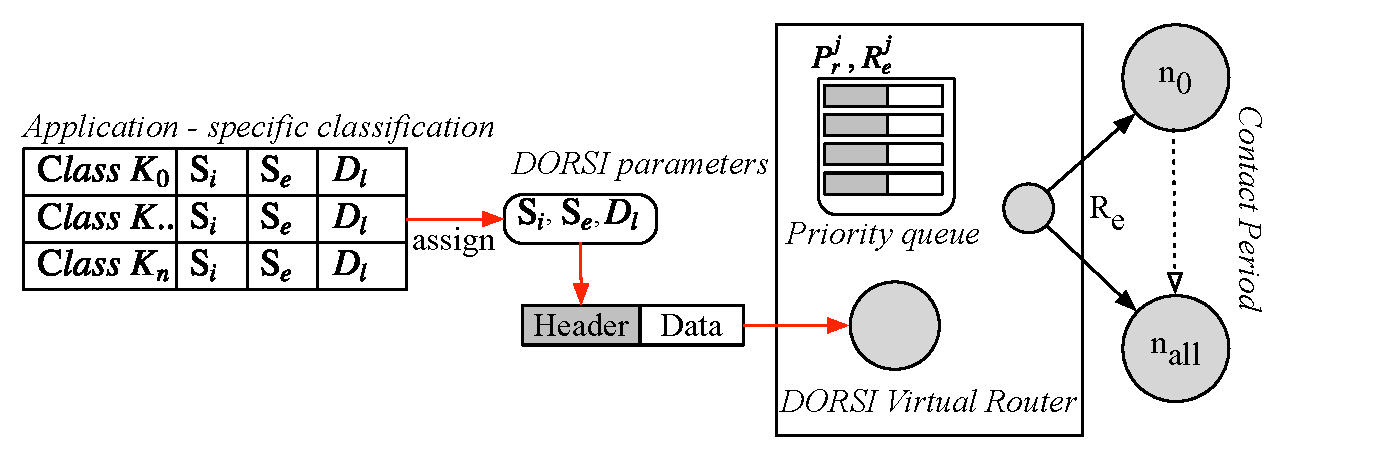
\includegraphics[width=5.5in]{Figures/DORSIsystemModel.pdf}
\caption{DORSI system model}
\label{DORSI system model}
\end{figure}

The design goal of DORSI is to distinguish the data with different information sensitivity concept. 
%%
We implement this protocol in order to guarantee that the important message can reach the destination within the time limit resulting in higher delivery ratio. 
%%
Additionally, we need to control the security risk of the message with higher security level by limiting the number of message replica in this network according with information sensitivity concept \cite{Kotrappa2010,marking2010}. 
%%
The final goal of this protocol is to increase the bandwidth efficiency by selecting the candidate nodes with higher probability of delivering the message to the destination.

Fig. \ref{DORSI system model} shows the proposed DORSI system model implemented as a virtual (software) router in an OppNet node. 
%%
In DORSI, besides common routing information such as source and destination addresses, every delivered message is associated with 3 additional DORSI parameters which are Significant level ($S_i$) Security level ($S_e$), Delivery deadline ($D_l$). 
%%
The $S_i$ represents how important of this message while the $S_e$ defines the level of this data that needs to be protected. 
%%
The $D_l$ element is the message expiration time. 
%%
If the delivery deadline is reached, the message will be dropped. 
%%
The value of these DORSI parameters are determined in accordance with the application specific requirement. 
%%
For example, the contents in military domain are divided into several classifications based on the multilevel of security which is intended to prevent unauthorized personnel from accessing information at higher classification than their authorization \cite{Winjum2008}. 
%%
Therefore, different classes of message in military perspective are treated differently.


At DORSI router, a time-constrained priority queue is used to carry DORSI messages waiting for being forwarded to the next node. 
%%
The DORSI parameters: $S_i$ , $S_e$ and $D_l$ are used in routing decision of DORSI virtual router on a node when this node opportunistically contacts to the other nodes. 
%%
Upon node contact, messages will be processed orderly according to their up-to-date priority value, however the message whose delivery deadline is reached will not be considered and will be removed out of the queue. 
%%
The priority value ($P_r^j$) of a specific message, $j$, is calculated based on its significant level and its expediting factor, $\xi(D_l^j, t)$, as in Eq. \ref{Eq:DORSI:routing algorithm}

\begin{eqnarray}
\label{Eq:DORSI:routing algorithm}
{ P }_{ r }^{ j }={ w }_{ p }{ S }_{ i }^{ j }+(1-{ w }_{ p })\xi ({ D }_{ l }^{ j },t)
\end{eqnarray}

where

\begin{equation*}
 \xi ({ D }_{ l }^{ j },t)=\begin{cases} 0;{ \tau  }_{ t }>{ \tau  }_{ max } \\ \frac { { \tau  }_{ max }-{ \tau  }_{ t } }{ { \tau  }_{ max }-{ \tau  }_{ min } }  \\ 1;{ \tau  }_{ t }<{ \tau  }_{ max } \end{cases};{ \tau  }_{ min }\le { \tau  }_{ t }\le { \tau  }_{ max } 	
\end{equation*}

The $W_p$ level and expediting factor components.
%%
We define $\tau_t$ as residual lifetime of message which is calculated from $D_t^j - t$. 
%%
The expediting factor value, in the range [0,1], is composed from the message
residual lifetime, compared with the maximum and minimum countable message lifetime, $\tau_{max}$ and $\tau_{min}$, in the system. 
%%
The message with the residual lifetime $\tau_t$ = $\tau_{max}$ is considered as no need to expedite the message delivery while the message with $\tau_{min}$ is considered for maximum expediting.
%%
Note that the $P_r^j$ value will be recalculated at every time any node get contacted. 
%%
When a specific message,$j$ , is being processed, the determination whether it should be copied and sent to a specific contact node is controlled by the replication probability value, $R_j^e$, calculated at a contact time as in Eq. \ref{Eq:DORSI:replication probability}.


\begin{eqnarray}
\label{Eq:DORSI:replication probability}
{ R }_{ e }^{ j }=(1-{ R }_{ min })[{ w }_{ r }{ P }_{ r }+(1-{ w }_{ r })(1-{ S }_{ e }^{ j })]+{ R }_{ min }
\end{eqnarray}

The replication probability value, in range of [${ R }_{ min }$, 1], is based on the concept that a message with
more priority, $P_r^j$, should be disseminated more in order to increase delivery ratio while the message with more security level should be replicated less in order to tighten security risk. 
%%
In the formula, the replication weight coefficient, $w_r$ , is used to balance effect between both components. 
%%
The ${ R }_{ min }$ is the minimum guaranteed replication probability value in the system so that even a message with very low priority and very high security still has a chance to be forwarded. 
%%
This ${ R }_{ min }$ is a configurable system parameter according to application requirement.
In case that there are several nodes simultaneously contacts when processing a specific message, the node with higher rank will be considered before the lower one. 
%%
The ranking value of a contacting node, 𝑛, is calculated according to its departure probability representing the relative chance to move away from the DORSI router node, $r$.

\begin{eqnarray}
\label{Eq:DORSI:node ranking model}
{ N }_{ r }^{ n }=\sqrt { { ({ x }_{ n }\cos { { \theta  }_{ n } } -{ x }_{ r }^{ t }\cos { { \theta  }_{ r }^{ t } } ) }^{ 2 }-{ ({ y }_{ n }\sin { { \theta  }_{ n } } -{ x }_{ r }^{ t }\sin { { \theta  }_{ r }^{ t } } ) }^{ 2 } } -\sqrt { { ({ x }_{ n }-{ x }_{ r }^{ t }) }^{ 2 }-{ ({ y }_{ n }-{ x }_{ r }^{ t }) }^{ 2 } } 
\end{eqnarray}

It can be estimated as the difference in distance between the current DORSI router, $r$, and the contacting node $n$ , after they moves further one unit distance in their current direction. 
%%
Given that the positions of the router $r$ and the contacting node $n$ are $(x_r,y_r)$ and $(x_n,y_n)$. 
%%
In addition, their moving direction vectors are 
$\vec { { d }_{ r } } =\cos { { \theta  }_{ r } } \hat { x } +\sin { { \theta  }_{ r } } \hat { y } $
and
$\vec { { d }_{ n } } =\cos { { \theta  }_{ n } } \hat { x } +\sin { { \theta  }_{ n } } \hat { y } $
, respectively. 
%%
The ranking value, $N_{r}^n$ is defined by formula in Eq. \ref{Eq:DORSI:node ranking model}. 
%%
The positive $N_{r}^n$ value means the contacting node is moving away while the negative value means that it becomes closer. 
%%
The contacting node with higher $N_{r}^n$ is needed to be considered since there is higher probability that it will be out of reach soon, compared with the other nodes. 
%%
In Fig. \ref{Eq:DORSI:node ranking model}, $D_0$ represents the distance between node $r$ and $n$ at time $t$ = 0 while $D_1$ is a distance at the time t=1. 
%%
If $D_1 > D_0$ , both nodes tend to move away from each other which results in higher node ranking.
%%
Note that all messages where lifetime reach their deadline are discarded from the carried node. 
%%
In addition, DORSI node will not receive the same copy of a specific message.

\begin{figure}[!t]
\centering
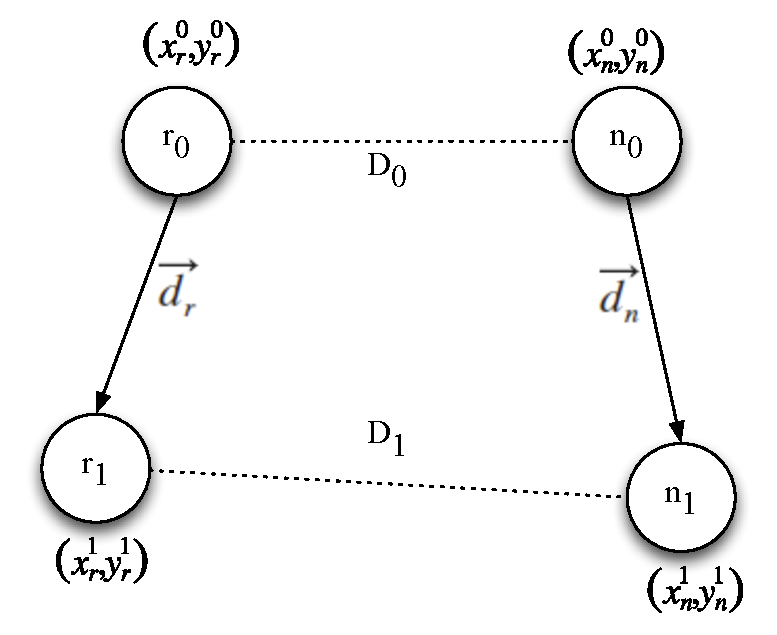
\includegraphics[width=4.5in]{Figures/NodeRankingModel.pdf}
\caption{Node ranking model}
\label{Node ranking model}
\end{figure}

%=============================================================================
\section{Evaluation}
\label{DORSI:Evaluation}
%=============================================================================
\begin{table}[!t]
		\renewcommand{\arraystretch}{1.3}
		\centering
		\begin{tabular}{|c|c|c|}
			\hline
			Parameters         & DORSI                  & Epidemic \\ \hline
			Operation Time     & \multicolumn{2}{|c|}{3600 Seconds }  \\ \hline
			Message Size       &           \multicolumn{2}{|c|}{500 KB - 5 MB}        \\ \hline
			Node Buffer        &              \multicolumn{2}{|c|}{1000 MB   }       \\ \hline
			Transmission Range &              \multicolumn{2}{|c|}{150 Meters  }        \\ \hline
			Transmission Speed &              \multicolumn{2}{|c|}{ 54 Mbps   }        \\ \hline
			Node Density       &                \multicolumn{2}{|c|}{0 - 100 \% }        \\ \hline
			Router             & DORSI                  & Epidemic \\ \hline
			Deadline                &  \multicolumn{2}{|c|}{Relative to data class}       \\ \hline
			Moving Speed       &          \multicolumn{2}{|c|}{0.5 - 1.5 m/s }        \\ \hline
			Movement Model     &       \multicolumn{2}{|c|}{Random Waypoint  }      \\ \hline
			Wait Time     &       \multicolumn{2}{|c|}{0 - 180 Seconds  }      \\ \hline
			Number of classes     &       \multicolumn{2}{|c|}{5 }      \\ \hline
		\end{tabular}
		\caption{DORSI Simulation variables}
		\label{TB:DORSI:table_parameters}
	\end{table}

\subsection{Simulation setup}
This protocol is designed to implement on any network that messages can be classified by data content. 
%%
We select the military tactical network as a sample application to present and evaluate this protocol because of its opportunistic behavior. 
%%
Since military tactical networks are subject to frequent disruption of end-to-end communication, current traditional network protocol tends to poorly handle these disruptive environment. 
%%
In this extreme scenario, opportunistic network with store-carry-forward scheme can be integrated into this tactical network to aid significant and secure operations. 
%%
In addition we employ MLS \cite{Winjum2008} as a classification of data in this military scenario environment, consisting of 5 classes.

We conduct the extensive simulations using the ONE 1.4.1 (The Opportunistic Network Environment simulator) \cite{Keranen2009b}. 
%%
ONE is a powerful JAVA tool for generating different movement models, running simulation with various routing protocols, visualizing simulations in real time and generating results, and post processing the results.

We implement new DORSI router with the designed simulation scenario to compare with modified traditional Epidemic routing protocol \cite{Vahdat2000}. 
%%
The Epidemic router is modified with the same classification as DORSI router in order to compare the actual performance between them. 
%%
However, the classification implemented in modified Epidemic router is not effected the message routing decision. 
%%
The Epidemic router treats every message the same while DORSI router routes messages differently according to their DORSI parameters. 
%%
Basically, the performance of opportunistic network correlates with the simulation parameters. 
%%
In our tactical network simulation environment, we implement the scenario corresponding to the actual military operation. 
%%
The common message in this tactical network traffic is usually commands in short message format, locations or images which the size of approximately 500 KB to 5 MB. 
%%
A mobile node is assumed to be a soldier equipped with modern communication equipment with transmission speed and range of 54 Mbps and 150 Meters respectively. 
%%
In addition, each node can hold up to 1 GB of storage for buffering the in-transmitted messages while randomly moving at a speed of 0.5 to 1.5 m/s. 
%%
The simulation time is set for 1 hour to study the behavior of messages inside the network traffic. 
%%
To evaluate the impact of message classification, we compare the performance of each router by varying the node density. 
%%
In random way point movement (RWP), nodes can move around in random zigzag paths. The nodes can move around randomly in a 1,000 m x 1,000 m area with walking speed. 
%%
In our experiment, the total number of nodes in a network per a one $km^2$ area denotes its node density. 
%%
Each message embedded with the deadline value correlative to the degree of that data sensitivity.

\subsection{Metric}
To evaluate DORSI with Epidemic routing protocol, we define two keys performance index corresponding to our design concept: Effective Delivery Ratio (EDR) and Effective Replication Ratio (ERR). 
%%
Our protocol disseminates the data by its degree of sensitivity, therefore in order to analyze actual performance this evaluation requires appending higher credential weight on the successful delivery of data with higher significant level. 
%%
Basically, delivery ratio is defined by the ratio of the total number of messages delivered to the total number of messages created. 
%%
In our evaluation, EDR can be computed by introducing significant level ($S_i$) into the number of delivered messages within the deadline ($M_d$) from each class to the number of created messages ($M_c$) as in equation \ref{Eq:DORSI:EDR}.

\begin{eqnarray}
\label{Eq:DORSI:EDR}
EDR=\frac { \sum _{ j=1 }^{ m }{ { S }_{ i }^{ j }{ M }_{ d }^{ j } }  }{ { M }_{ c }^{ j } } 
\end{eqnarray}

On the other hand, we can compute ERR by the number of replicated messages ($M_r$) that incorporate with security level ($S_e$) to the total created messages as in equation \ref{Eq:DORSI:ERR}. 
%%
The higher ERR means more message replicas in the network resulting in excessive network resource consumption and higher security risk.

\begin{eqnarray}
\label{Eq:DORSI:ERR}
ERR=\frac { \sum _{ j=1 }^{ m }{ { S }_{ e }^{ j }{ M }_{ r }^{ j } }  }{ { M }_{ c }^{ j } } 
\end{eqnarray}

%%%%%%%%%%%%%%%%%%%%%%%%%%%%%%%%%%%%%%%%%%%%%%%%%%%%%%%%%%%%%%%%%%%%
\subsection{Result}
%%%%%%%%%%%%%%%%%%%%%%%%%%%%%%%%%%%%%%%%%%%%%%%%%%%%%%%%%%%%%%%%%%%%

\begin{figure}[!h]
\centering
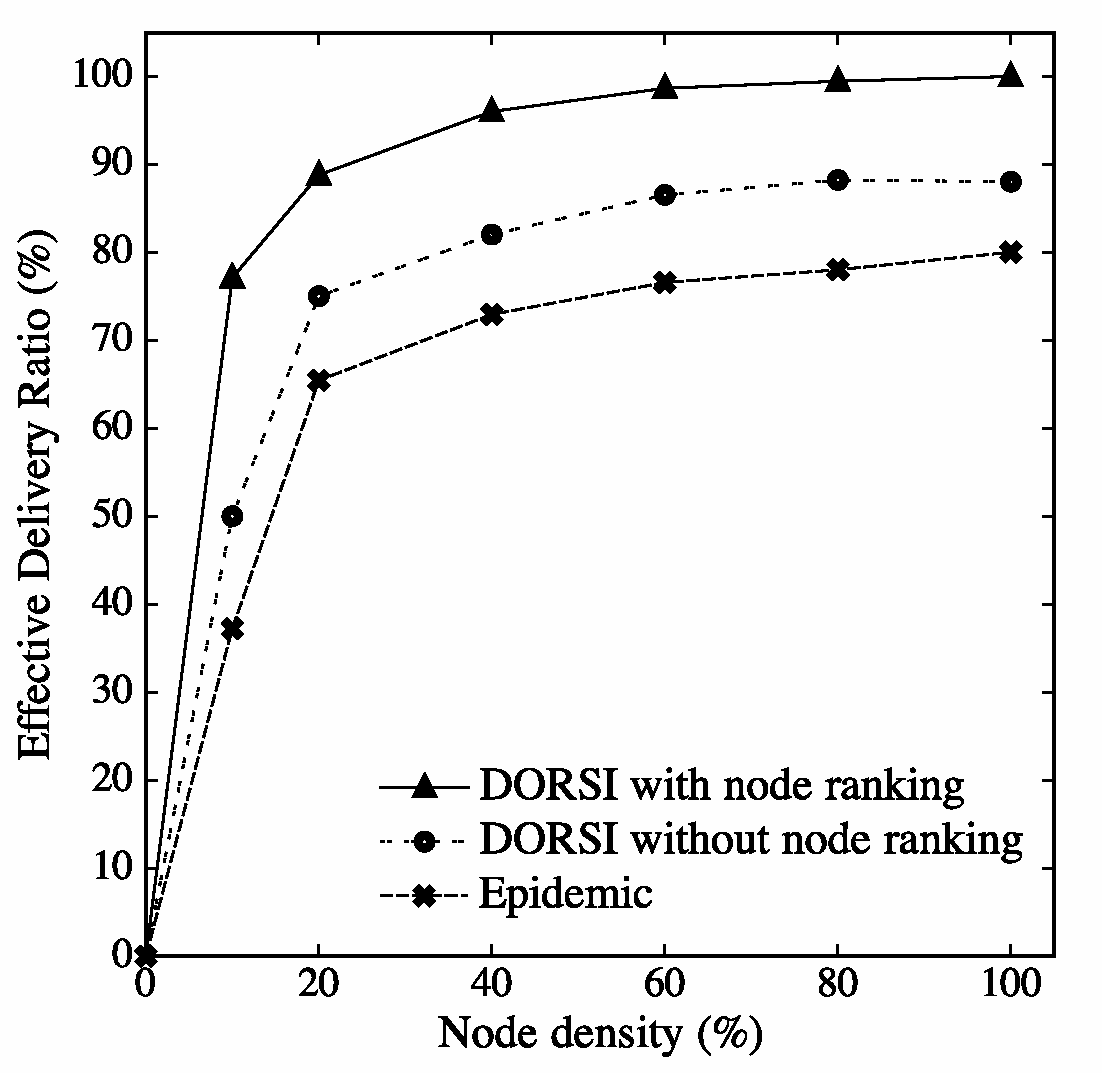
\includegraphics[width=3in]{Graphs/EDR_NodeDensity.pdf}
\caption{Effective Delivery Ratio comparison}
\label{Fig:DORSI:Effective Delivery Ratio comparison}
\end{figure}

Our implementation consists of two presenting keys: deliverable of significant data and security risk. 
%%
Firstly, we analyze the EDR value to determine the delivery guarantee for important data. 
%%
Figure \ref{Fig:DORSI:Effective Delivery Ratio comparison} presents the relationship between effective delivery ratio and node density comparing DORSI to epidemic routing. 
%%
This graph illustrates that DORSI gains remarkably higher EDR than the Epidemic, approximately 35\%. 
%%
By the common nature of flooding based routing, the EDR increases with the node density because node can obtain higher tendency of successful message delivery when the number of nodes increase. 
%%
In addition, at sparse node density condition (less than 10\%), the EDRs of 3 simulated routing protocols are similar because of our prioritization technique requires specific amount of nodes in order to efficiently perform. 
%%
Nevertheless, achieving 100\% EDR is impractical even though all resource is utilized for this purpose. 
%%
Message prioritization can improve the overall EDR about 10\% over epidemic while node ranking mechanism can increase approximately more 25\% EDR than DORSI without node ranking.

\begin{figure}[!h]
\centering
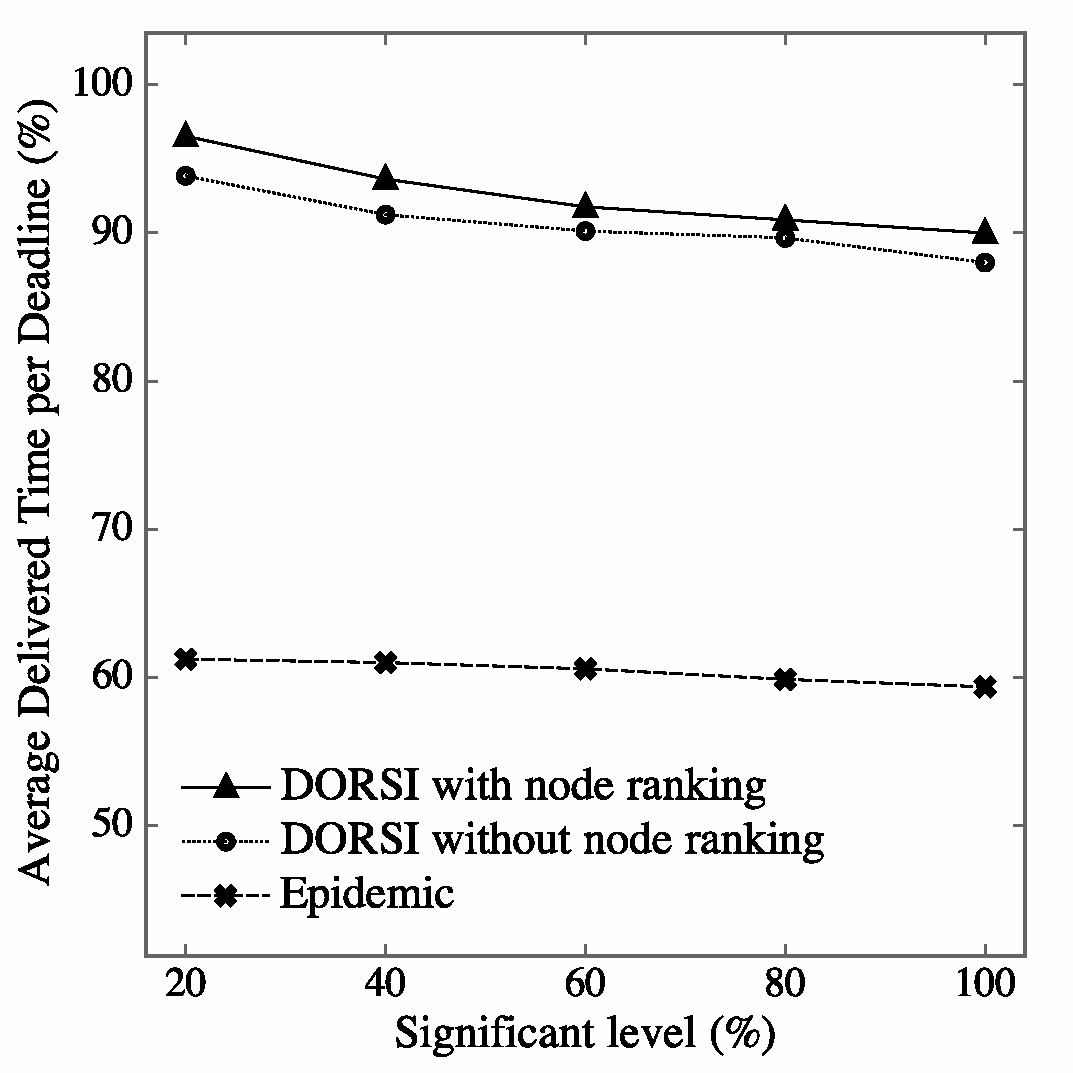
\includegraphics[width=3in]{Graphs/ADTD_significantLevel.pdf}
\caption{Average Delivered Time per Deadline on Significant Level}
\label{Fig:DORSI:Average Delivered Time per Deadline on Significant Level}
\end{figure}

As a result, DORSI outperforms Epidemic due to these design components: Firstly, by introducing deadline into our message prioritization method, the message with higher significant level can reach the destination faster. 
%%
This concept is supported by the Average Delivered Time (ADT) per deadline to significant level as shown in Fig. \ref{Fig:DORSI:Average Delivered Time per Deadline on Significant Level}. This graph presents that the messages routing with DORSI can reach the destination closer to their deadline than epidemic counterpart. 
%%
The consequence from Fig. \ref{Fig:DORSI:Effective Delivery Ratio comparison} and \ref{Fig:DORSI:Average Delivered Time per Deadline on Significant Level} shows that higher EDR of DORSI is a result from optimizing the time of delivery to their deadline.

\begin{figure}[!h]
\centering
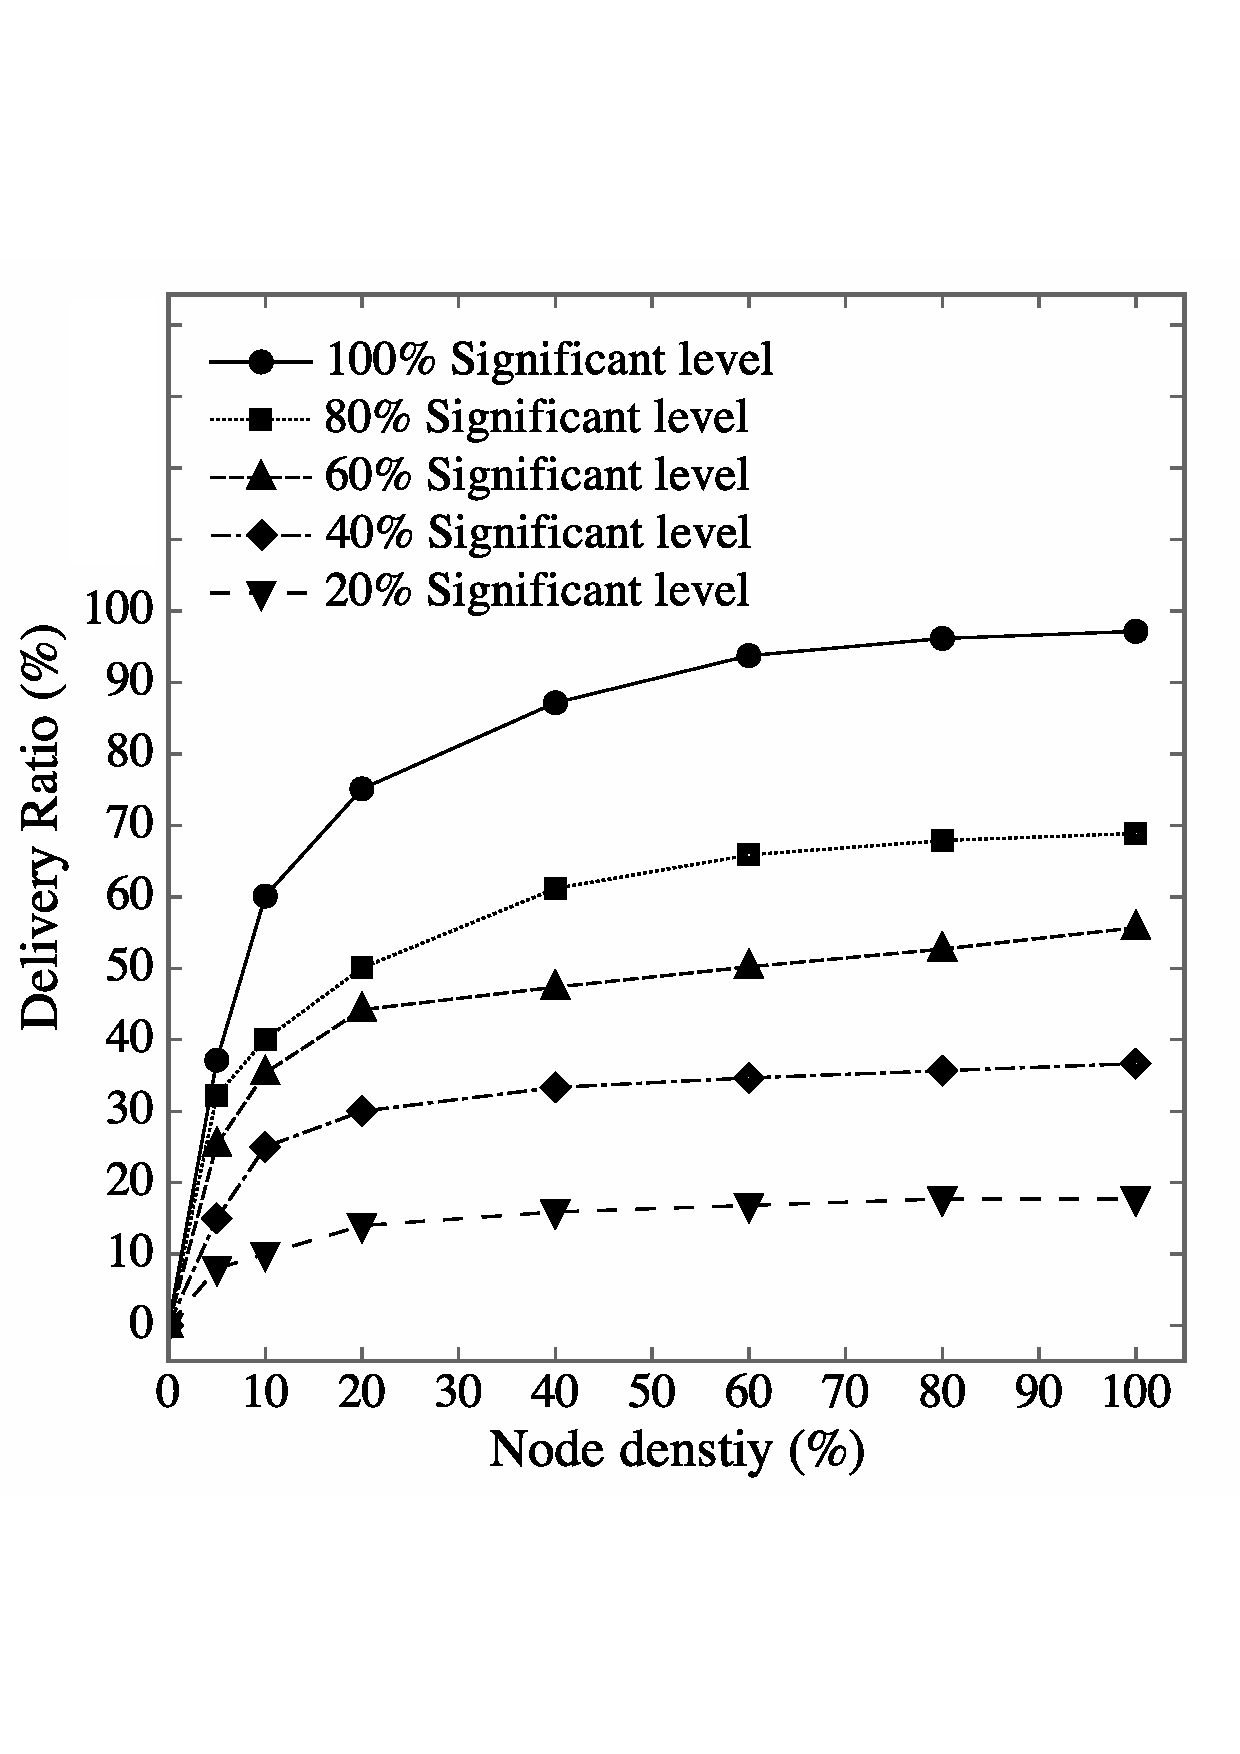
\includegraphics[width=3in]{Graphs/DR_NodeDenstiy2.pdf}
\caption{DORSI Delivery Ratio on each class}
\label{Fig:DORSI:DORSI Delivery Ratio on each class}
\end{figure}

Message prioritization technique can increase the delivery ratio of important data as in Fig. \ref{Fig:DORSI:DORSI Delivery Ratio on each class}. 
%%
This graph shows the relationship between delivery ratios of each class in DORSI to the node density. 
%%
Normally, messages with higher significant level (such as top secret or secret data) obtain more chance of successfully reaching the destination than others. The result clearly suggests that the delivery ratio of data with higher significant level is higher than less important data. 
%%
Comparing delivery ratio on each class of DORSI and Epidemic, the message prioritization can distinguish the significant level of messages. 
%%
On the other hand, the delivery ratio of all classes on Epidemic routing in Fig. \ref{Fig:DORSI:Epidemic Delivery Ratio on each class} are similar while the delivery ratio of DORSI increases by its classes. 
%%
Consequently, the message prioritization can control the delivery time of each class resulting in overall deliverable improvement.

\begin{figure}[!h]
\centering
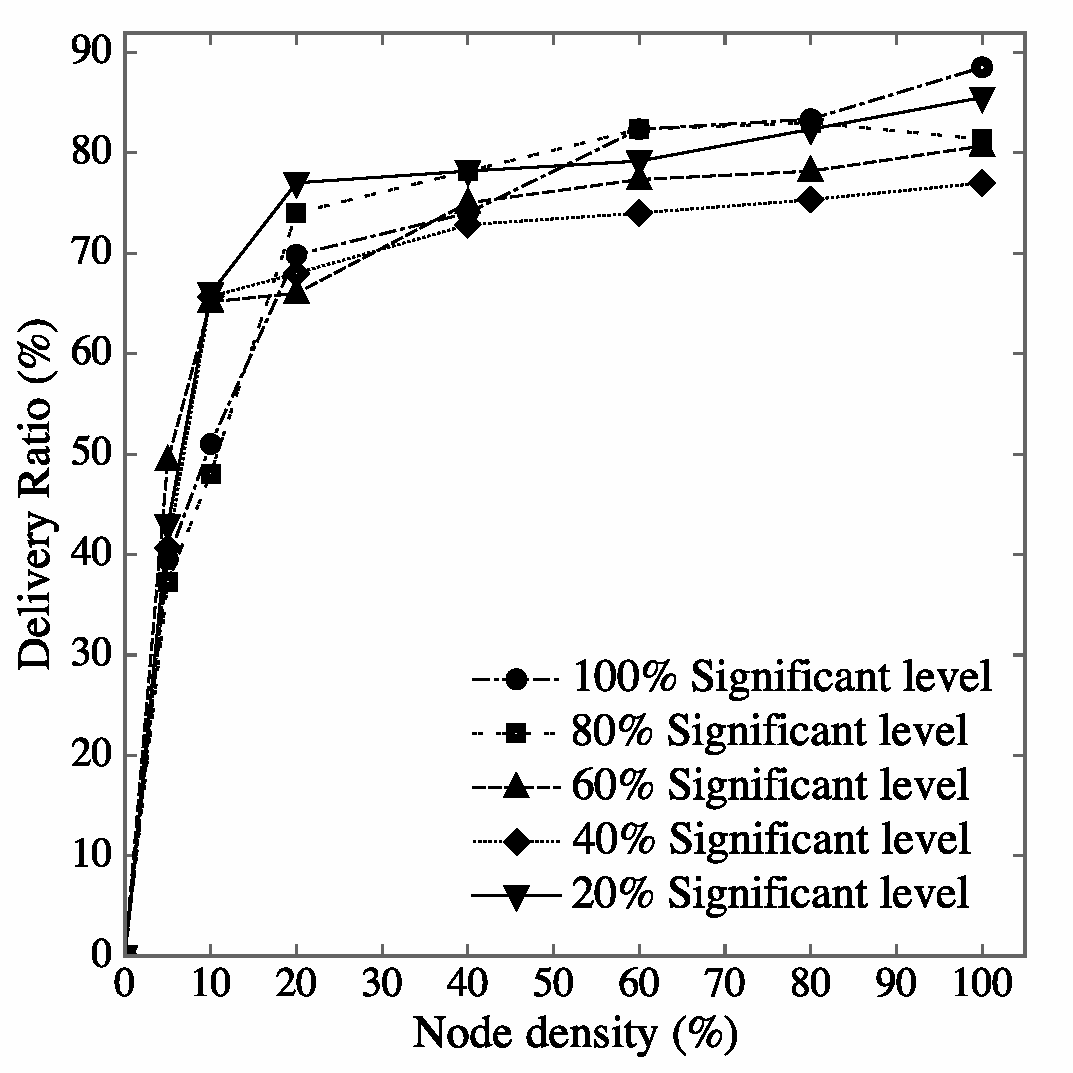
\includegraphics[width=3in]{Graphs/EpidemicDeliveryRatiooneachclass.pdf}
\caption{Epidemic Delivery Ratio on each class}
\label{Fig:DORSI:Epidemic Delivery Ratio on each class}
\end{figure}

Node ranking mechanism can enhance more EDR of DORSI over this same protocol without node ranking. 
%%
By selecting the best candidate nodes to transmit the data, the important messages can gain more chance of reaching the destination. 
%%
Fig. \ref{Fig:DORSI:Effective Delivery Ratio comparison} and \ref{Fig:DORSI:Effective Replication Ration Comparison} clearly shows that the node selecting technique can improve the performance of DORSI without node ranking. 
%%
This significantly benefits the network resource consumption and higher chance of deliverable of important data.

\begin{figure}[!h]
\centering
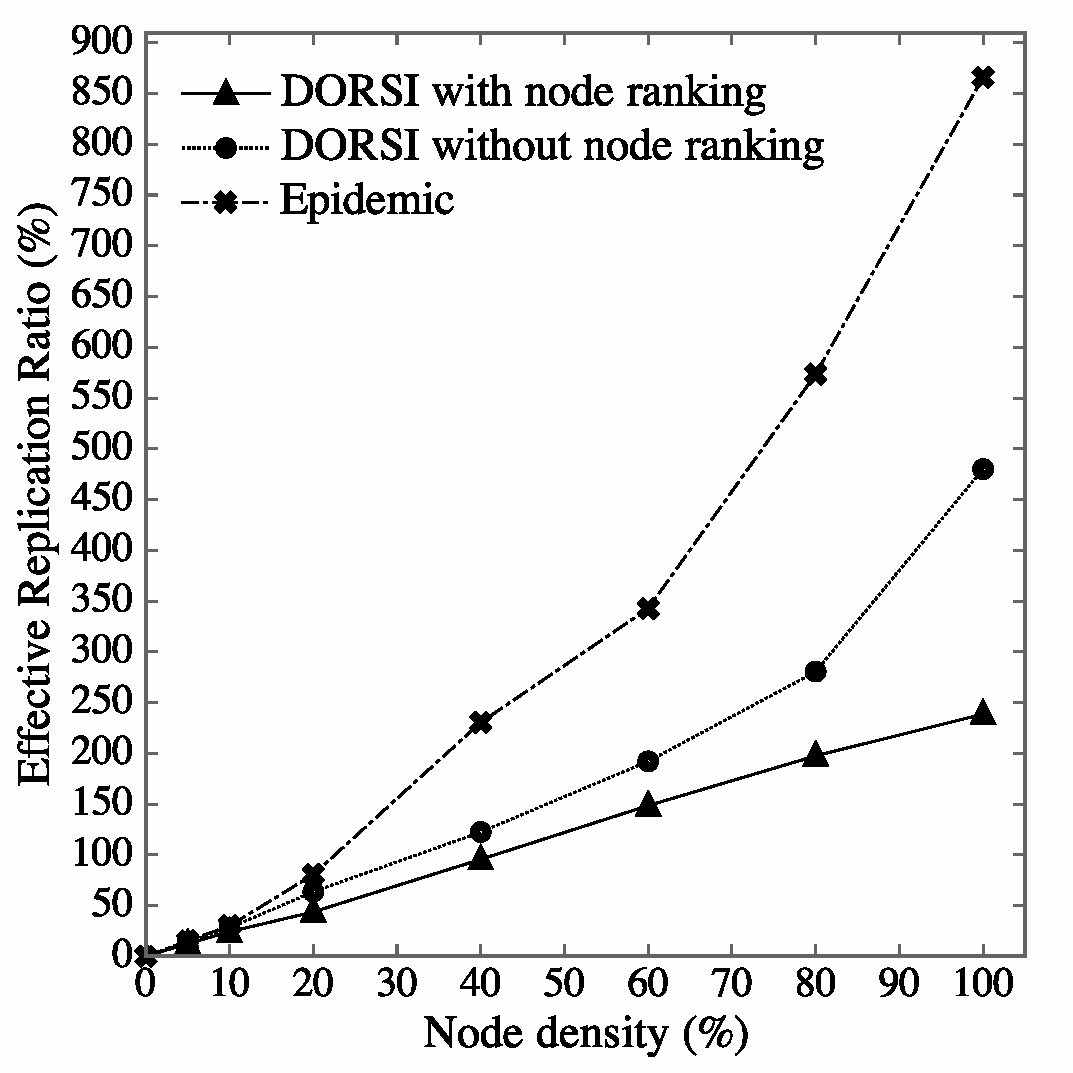
\includegraphics[width=3in]{Graphs/EffectiveReplicationRationComparison.pdf}
\caption{Effective Replication Ratio Comparison}
\label{Fig:DORSI:Effective Replication Ration Comparison}
\end{figure}

On the other hand, the ERR is analyzed to assess the security risk. 
%%
The ERR of Epidemic and DORSI without node ranking exponentially increase while DORSI with node ranking gradually rises as in Fig. \ref{Fig:DORSI:Effective Replication Ration Comparison}. 
%%
This graph shows the relationship between effective replication ratio and node density. 
%%
The lower number of ERR means that less message replicas in the network resulting in less security risk. 
%%
Because the DORSI protocol can efficiently control the number of message replication in the network traffic, the number of message copies are remarkably lower than Epidemic. 
%%
This result proves our design concept of security risk and aids in the optimum network bandwidth utilization.

To study the behavior of our protocol, we analyze the result of various number of classes as well. 
%%
In our scenario, we divide the data class based on British MLS scheme with 5 level of security: Top Secret (T), Secret (S), Restrict (R), Confidential (C) and Unclassified (U). 
%%
However, there are other MLS schemes for different zone of military, for example, the US. 
%%
DoD employs only 4 level of security: T, S, C and U. In order to deploy our method to different class of data, we simulate the data with different scale of classes. 
%%
Fig. \ref{Fig:DORSI:EDR on different classification scale} shows the comparison of effective delivery ratio and node density between different class scales from 1 to 5 classes. 
%%
This graph shows the similar trend between all classes which is the more node density the higher the delivery ratio. 
%%
The overall EDR increases when the messages are classified with more number of classes. 
%%
This is the outcome from DORSI routing which requires some node amount to process the node ranking mechanism. 
%%
This result proves that the classification technique can be deployed to various number of classes in any application.

\begin{figure}[!h]
\centering
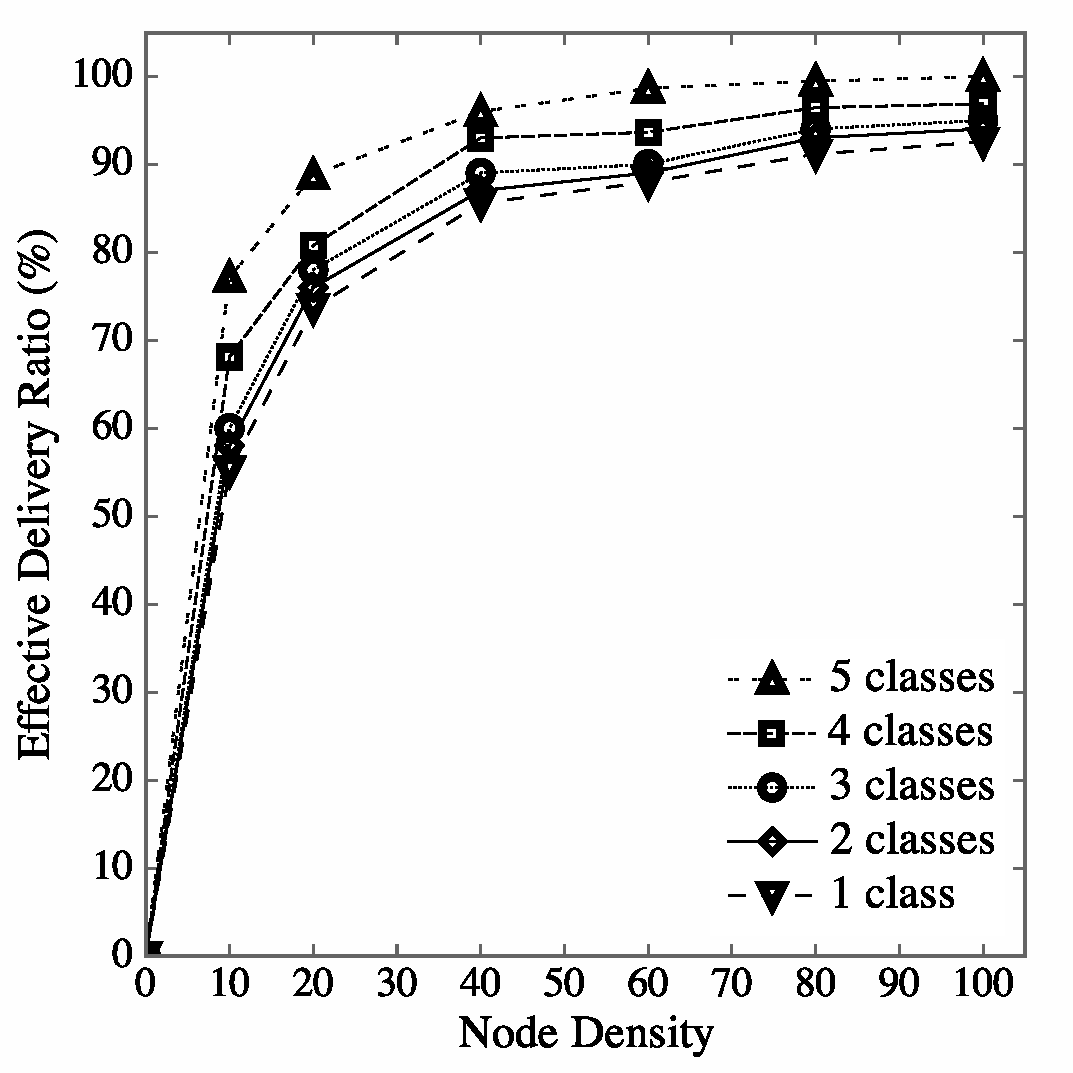
\includegraphics[width=3in]{Graphs/EDRondifferentclassificationscale.pdf}
\caption{EDR on different classification scale}
\label{Fig:DORSI:EDR on different classification scale}
\end{figure}

To study the behavior of DORSI, we select 20\% node density scenario aiming to analyze its performance by varying the transmission range of simulation parameters. 
%%
Fig. \ref{Fig:DORSI:EDR comparing varied by transmission range} presents the relationship of EDR to the node transmission range. 
%%
The result shows that the EDR increase with transmission range especially after 50 meters. 
%%
However after the range of 150 meters, the EDR tends to slightly decline. 
%%
By increasing the transmission range, transmitting node in DORSI can increase its opportunity to selecting the candidate nodes, resulting in more chance of reaching destination.

\begin{figure}[!h]
\centering
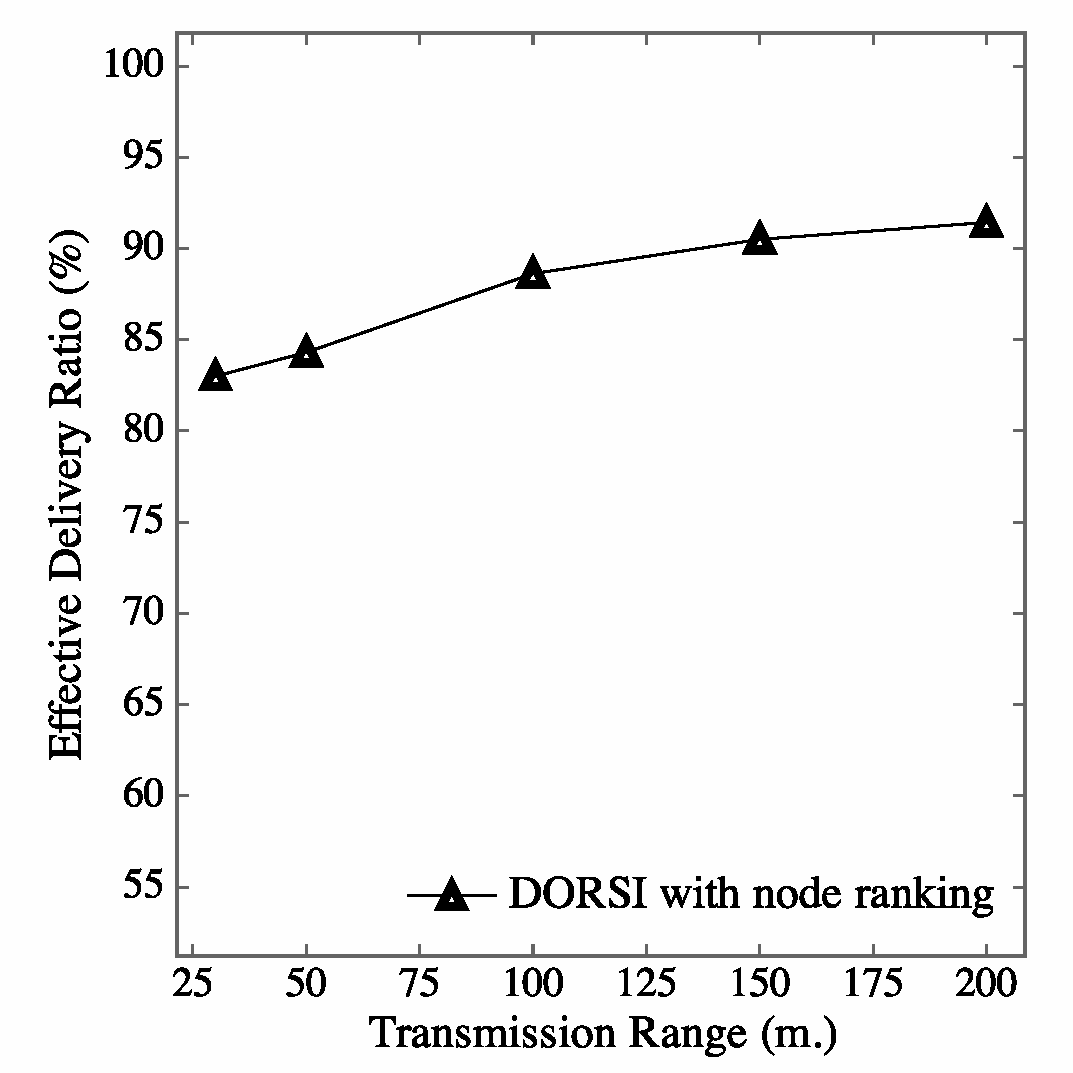
\includegraphics[width=3in]{Graphs/EDRcomparingvariedbytransmissionrange.pdf}
\caption{EDR comparing varied by transmission range}
\label{Fig:DORSI:EDR comparing varied by transmission range}
\end{figure}

All in all, the key performance from simulation results confirms with our design goals. 
%%
In DORSI, the value of EDR and ERR shows that we can control the message replication thus the message with higher priority can reach the destination faster to prove the concept of significant level and security level. 
%%
In addition, the value of ADT proves that we can control the messages to reach the destination near their expiration. 
%%
Normally, the delivery ratio increases with the number of message copies.
%%
However, our approach can maintain the delivery ratio while reducing the message replicas in the network. 
%%
As a result, this method significantly optimizes the network utilization. 
%%
The drawback of this protocol is high processing time since these executable nodes require amount of computation time.

%=============================================================================
\section{Conclusion}
\label{DORSI:Conclusion}
%=============================================================================
In this chapter, we propose a novel Data-wise Opportunistic Routing with Spatial Information (DORSI) in order to classify the messages based on the information sensitivity concept along with nodes prioritization technique corresponding to the their delivery probability computed by spatial data. 
%%
This protocol classifies the messages according to their significant level, security level and deadline relative to the sensitivity level of data. 
%%
Meanwhile, this chapter adapts the geographical routing technique to select the best candidate node to forward the messages to the destination. 
%%
Simulation experiments clearly illustrate that two key performance indexes — effective delivery ratio and effective replication ratio — remarkably improve over the traditional Epidemic routing. Moreover, the delivery ratio of DORSI and Epidemic comparison shows notable overall enhancement of the network routing efficiency. 
%%
This means that DORSI protocol can guarantee higher delivery ratio on more important data while limiting the replication of data with higher security level. 
%%
The average delivered time of DORSI also shows the optimal bandwidth utilization since it can control the messages to reach the destination closer to their deadline. 
%%
In addition, this method can be applied to different scale of data classification to suit any application deployment. 
%%
Furthermore, our work can be extended in various directions. 
%5
An obvious extension of the work could be the evaluation of our approach on a virtualization network to physically obtain the real life results comparing to the results from this simulation result. 
%%
Next, we will evaluate the performance of our method in different conditions in order to apply data classification routing technique on more general applications.
%%











































    
\chapter{Conclusion and Future Work}
\label{cf}
% \SVN $Revision: 838 $
% \SVN $Author: sgordon $
% \SVN $Date: 2014-05-12 13:30:42 +0700 (Mon, 12 May 2014) $
% \SVN $URL: https://sandilands.info/svn/Common/Styles/siitthesis/chapter2.tex $




%=============================================================================
\section{Discussion}
\label{cf:Discussion}
%=============================================================================


%=============================================================================
\section{Conclusion}
\label{cf:Conclusion}
%=============================================================================



%=============================================================================
\section{Future Work}
\label{cf:Future Work}
%=============================================================================












%%%%%%%%%%%%%%%%%%%%%%%%%%%%%%%%%%%%%%%%%%%%%%%%%%%%%%%%%%%%%%%%%%%%%%%%%%%%%% 
%
% References
% (\bibliography refers to your BibTeX .bib file, e.g. refs.bib)
%
%%%%%%%%%%%%%%%%%%%%%%%%%%%%%%%%%%%%%%%%%%%%%%%%%%%%%%%%%%%%%%%%%%%%%%%%%%%%%% 
\backmatter
\cleardoublepage % needed to ensure TOC page number is correct
%% There is still a bug with the PDF hyperlink: clicking on the References
%% link in the PDF takes you to last page of previous chapter, not to start
%% of references
\addcontentsline{toc}{section}{References}

%% These two commands are for when using BibTeX (i.e. most common)
%% Change 'refs' to be the name of your .bib file
\bibliographystyle{abbrv}
\bibliography{refs}

%% In the final version of your thesis you may copy the generated .bbl file
%% to a .tex file (e.g. copy thesis.bbl to refs.tex) and input that .tex 
%% file. This allows you to make minor manual edits to the references.
%% Uncomment the following line; comment out the two above commands.
%\input{refs}


%%%%%%%%%%%%%%%%%%%%%%%%%%%%%%%%%%%%%%%%%%%%%%%%%%%%%%%%%%%%%%%%%%%%%%%%%%%%%% 
%
% Appendices
% (edit the files appendixA.tex, appendixB.tex, ...)
%
%%%%%%%%%%%%%%%%%%%%%%%%%%%%%%%%%%%%%%%%%%%%%%%%%%%%%%%%%%%%%%%%%%%%%%%%%%%%%% 
\appendix
\chapter{List of Publications}
\label{app1}
% \SVN $Revision: 840 $
% \SVN $Author: sgordon $
% \SVN $Date: 2014-05-12 13:39:14 +0700 (Mon, 12 May 2014) $
% \SVN $URL: https://sandilands.info/svn/Common/Styles/siitthesis/appendixA.tex $


\paragraph{International Journals}

\begin{itemize}
\item Jiradett Kerdsri, Komwut Wipusitwarkun, "Dynamic Rendezvous based Routing Algorithm on Sparse Opportunistic Network Environment", \textit{International Journal of Distributed Sensor Networks}, Vol. x, No. xx, pp. xx-xx, 2015 (in ISI, impact factor=0.923)
(To appear)
  \item Jiradett Kerdsri, Komwut Wipusitwarkun, "DORSI: Data-wise Opportunistic Routing with Spatial Information", \textit{JCIT: Journal of Convergence Information Technology}, Vol. 8, No. 13, pp. 91-103, 2013 (in SCOPUS)
\end{itemize}


\paragraph{International Conferences}

\begin{itemize}
\item Jiradett Kerdsri, Komwut Wipusitwarkun, "Rendezvous Based Routing in Opportunistic Networks" \textit{The Third International Conference on Informatics Engineering and Information Science (ICIEIS2014)}, pp.121-126, 22-24 Sep. 2014
\item Jiradett Kerdsri, Komwut Wipusitwarkun, "Data-wise Routing in Virtualization Environment (DRIVE) with multiple level of security for tactical network" \textit{2012 IEEE/SICE International Symposium on System Integration (SII)}, pp.933-938, 16-18 Dec. 2012
\item Jiradett Kerdsri, Komwut Wipusitwarkun, "Network virtualization for military application: Review and initial development of conceptual design", \textit{14th International Conference on Advanced Communication Technology (ICACT)}, pp.61-66, 19-22 Feb. 2012  
\end{itemize}
%\input{appendixB}
%\input{appendixC}

\end{document}

